\documentclass{beamer}
%\documentclass[handout]{beamer}
\usepackage[ngerman]{babel}
\usepackage[utf8]{inputenc}
\usepackage{graphicx}
\usepackage{tikz}
\usepackage[matrix,arrow]{xy}
\usepackage{amsmath}
\usepackage{amssymb}
\usepackage{dsfont}
\usepackage{hyperref}

%\usepackage[T1]{fontenc}
%\usepackage[english]{babel}
%\usepackage[fixlanguage]{babelbib}
%\usepackage{multimedia}



\usetheme{Warsaw}
%\useinnertheme{rounded}
\useoutertheme{infolines}
%\setbeamercovered{transparent}

\title[DEC]{Diskretes Äußeres Kalkül (DEC)\\auf Oberflächen ohne Rand}
\author{Ingo Nitschke}
\institute{IWR - TU Dresden}
\date{25. September 2014}

\beamertemplatenavigationsymbolsempty

\newcommand{\R}{\mathds{R}}
\newcommand{\Z}{\mathds{Z}}
\newcommand{\csd}{\text{csd}}
\renewcommand{\div}{\text{Div}}
\renewcommand{\hom}{\text{Hom}}
\newcommand{\err}{\text{Err}}
\newcommand{\id}{\text{Id}}
\newcommand{\D}{\text{D}}
\renewcommand{\d}{\mathrm{d}}
\newcommand{\exd}{\mathbf{d}}
\newcommand{\argmin}{\operatornamewithlimits{argmin}}
\newcommand{\sgn}{\mathop{\mathrm{sgn}}\nolimits}
\newcommand{\formpunkt}{\,\text{.}}
\newcommand{\formkomma}{\,\text{,}}
\newcommand{\formtext}[1]{\quad\text{#1}\quad}
\newcommand{\eps}{\varepsilon}
\newcommand{\vecflat}[1]{\vec{#1}^{\,\flat}}
\newcommand{\vecover}[2]{\vec{#1}^{\,#2}}
\newcommand{\diag}[1]{\text{diag}\left( #1 \right)}
\newcommand{\II}{I \! I}
\newcommand{\av}{\text{Av}}
\newcommand{\conn}{\text{Conn}}
\newcommand{\tred}[1]{\textcolor{red}{#1}}


\begin{document}
 \frame{ \titlepage }
 \frame {
    \frametitle{Content}
    \tableofcontents
  }

  
\section{Differentialformen und Motivation}

  \begin{frame}
    \begin{block}{"`Tensor-Maschine"'}
      Für einen Vektorraum \( V \) nimmt ein \( (m,n) \)-Tensor \( m \) Kovektoren aus \( V^{*} \)
      (Dualraum von \( V \)) und \( n \) Vektoren aus \( V \) und gibt einen Wert aus \( \R \) zurück.

      \hfill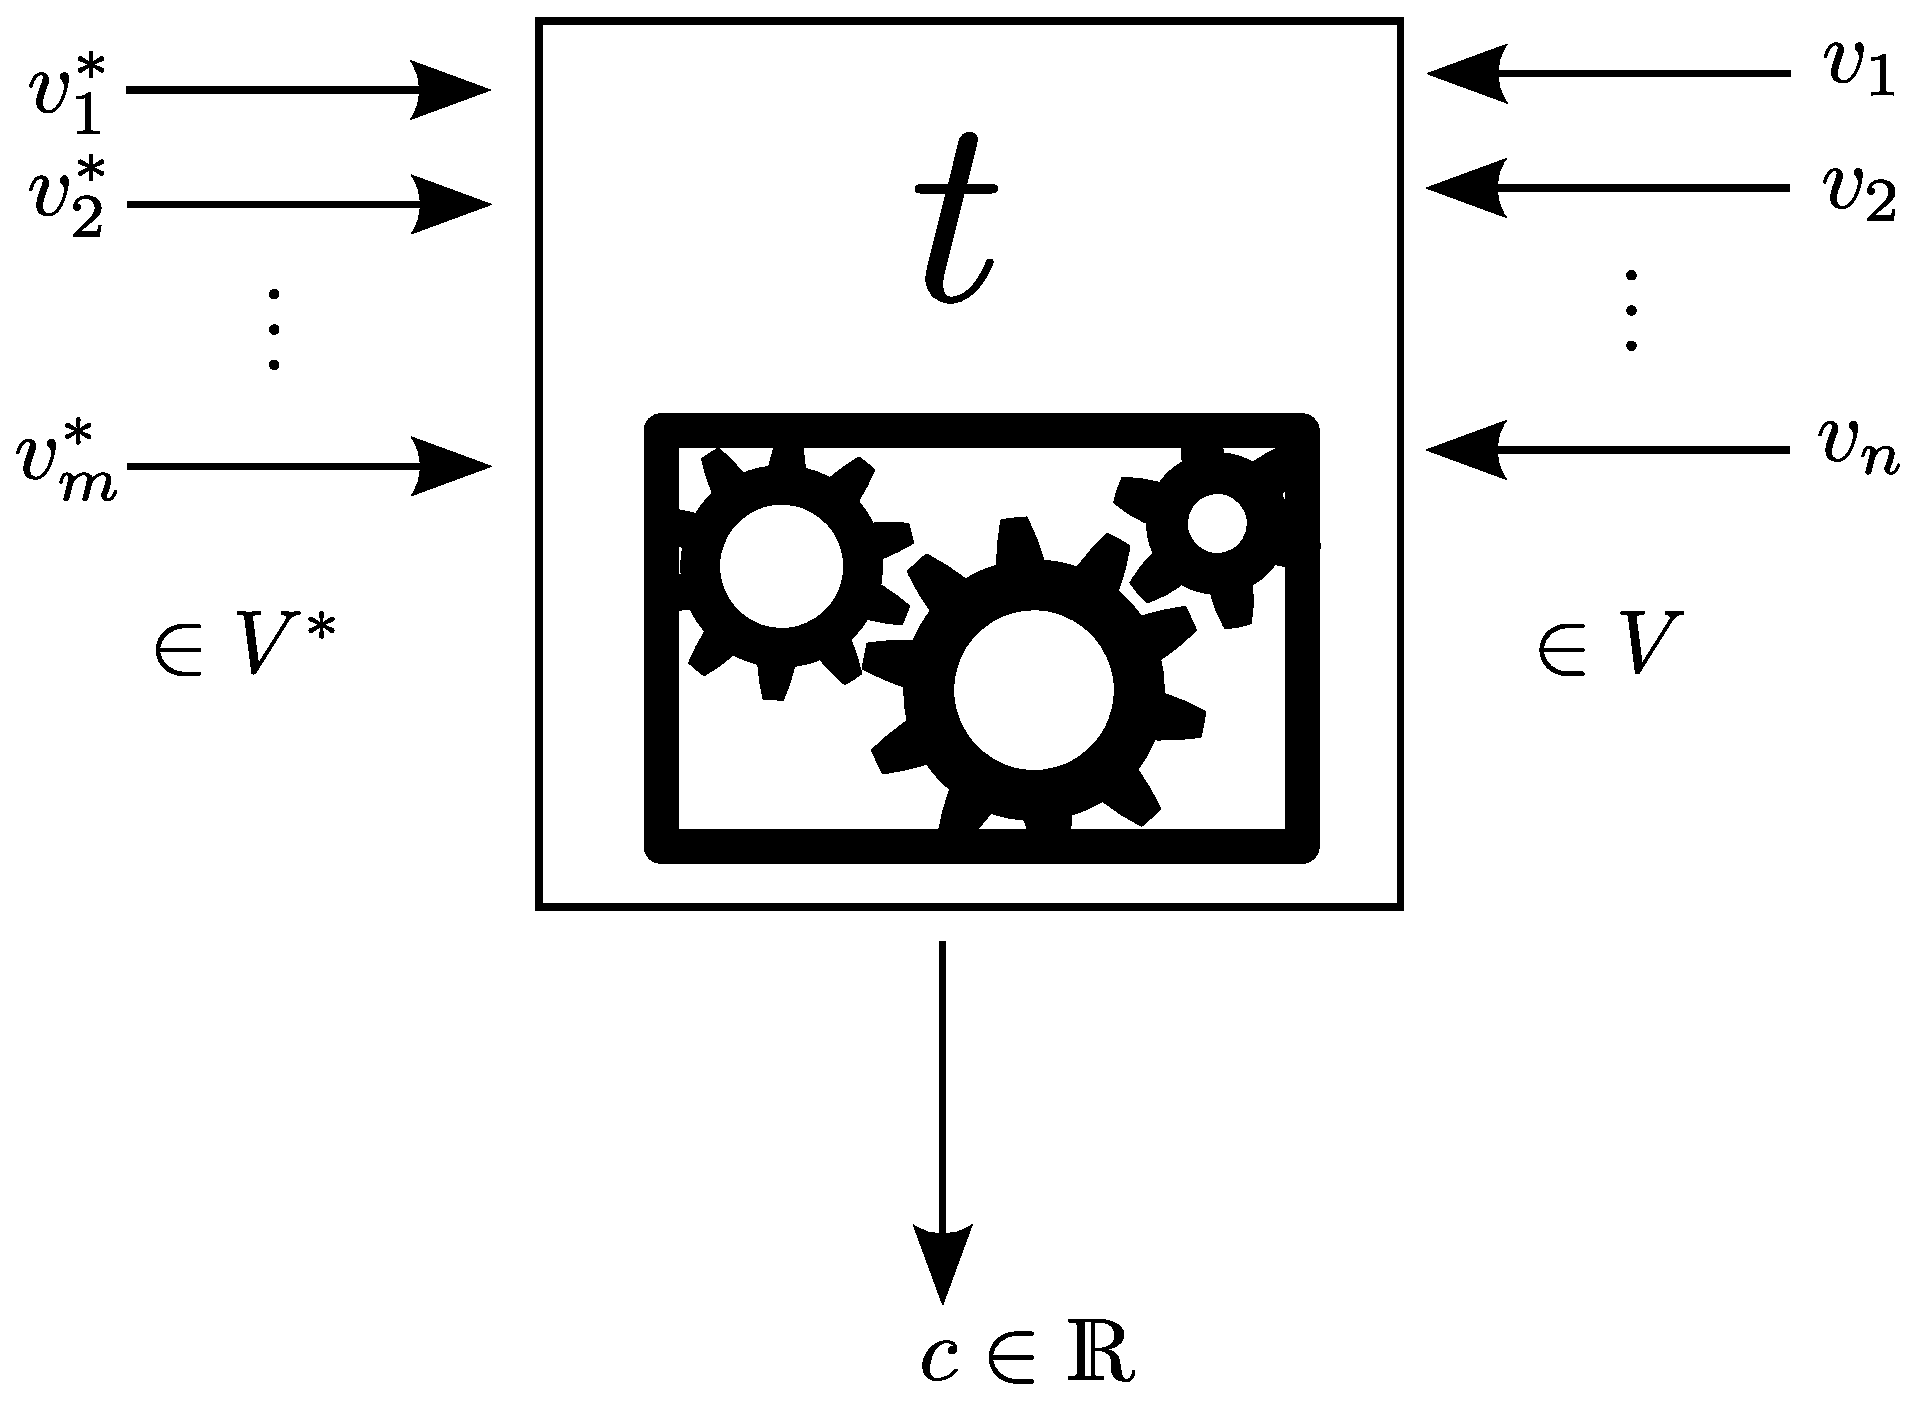
\includegraphics[height=0.7\textheight]{bilder/tensormaschine/Tensor.eps}\phantom{qwertz}
    \end{block}
  \end{frame}

  \begin{frame}
    \begin{block}{Differentialform als "`Tensor-Maschine"'}
      Eine Differentialform vom Grad \( n \) ist ein antisymmetrischer \( (0,n) \)-Tensor.

      \hfill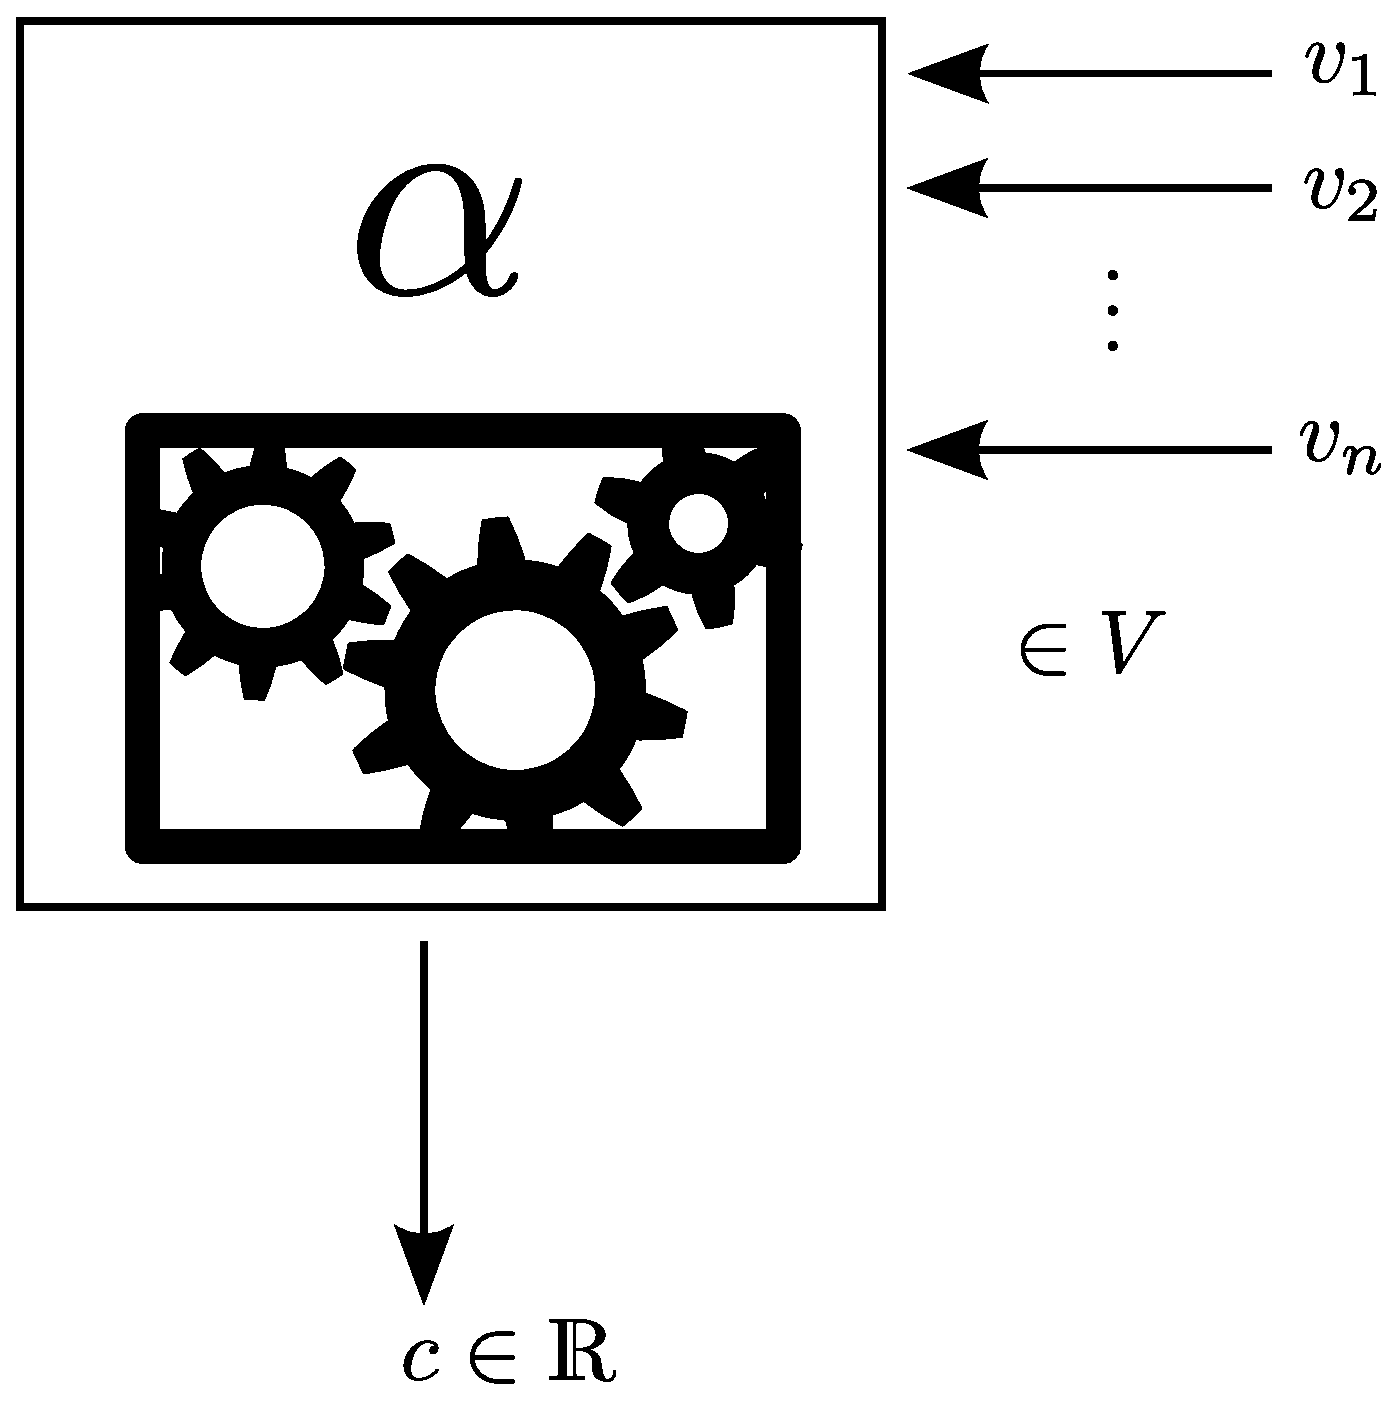
\includegraphics[height=0.7\textheight]{bilder/tensormaschine/Differentialform.eps}\phantom{qwertz}
    \end{block}
  \end{frame}

  %\begin{frame}
  %  \begin{block}{Beispiel im \( \R^{2} \supseteq U\), \( dim(U) = 2 \)}
  %    \begin{description}
  %      \item[0-Formen] \( f:\emptyset\rightarrow\R \) sind Konstanten
  %        bzw. Funktionen.
  %        \begin{align*}
  %          f:U\rightarrow\R,\ x\mapsto f_{x}:=f(x) \formpunkt
  %        \end{align*}
  %      \item[1-Formen] \( \alpha\in\left( \R^{2} \right)^{*}\cong\R^{2}  \) können als Zeilenvektoren (Kovektoren)
  %        aufgefasst werden
  %        \begin{align*}
  %          \alpha = \left[ \alpha_{1},\alpha_{2} \right]:\R^{2}&\rightarrow\R \\ 
  %                 \vec{v} = \begin{bmatrix}
  %                  v^{1} \\ v^{2}
  %                 \end{bmatrix}
  %                 &\mapsto \alpha(v) = \left[ \alpha_{1},\alpha_{2} \right] \begin{bmatrix}
  %                        v^{1} \\ v^{2}
  %                        \end{bmatrix}
  %                 = \alpha_{1}v^{1} + \alpha_{2}v^{2}
  %        \end{align*}
  %        bzw. als Zeilenvektorfeld
  %        \begin{align*}
  %          \alpha: U\times\mathcal{V}(U)&\rightarrow\R\\
  %                \left( x,\vec{v} \right)&\mapsto\alpha_{x}(\vec{v})=\alpha_{1}(x)v^{1}(x) + \alpha_{2}(x)v^{2}(x)
  %        \end{align*}
  %      \item[2-Formen] können als antisymmetrische Matrizen aufgefasst werden.
  %    \end{description}
  %  \end{block}
  %\end{frame}

  %\begin{frame}
  %  \begin{block}{Metrischer Tensor zweidimensionaler Mannigfaltigkeiten}
  %    \begin{itemize}
  %      \item o.E.d.A orthogonal:
  %            \begin{align*}
  %              g =\begin{bmatrix}
  %                g_{1} & 0 \\
  %                0 & g_{2}
  %              \end{bmatrix}
  %            \end{align*}
  %      \item Skalarprodukt:
  %        \begin{align*}
  %          \left\langle \vec{w}, \vec{v} \right\rangle_{g} = \vec{w}^{T} g \vec{v} = g_{1}w^{1}v^{1} + g_{2}w^{2}v^{2}
  %        \end{align*}
  %      \item Länge: 
  %        \begin{align*}
  %          \left\| \vec{v} \right\|_{g} = \sqrt{\left\langle \vec{v}, \vec{v} \right\rangle_{g}}
  %        \end{align*}
  %      \item Winkel:
  %        \begin{align*}
  %          \cos\Theta = \frac{\left\langle \vec{w}, \vec{v} \right\rangle_{g}}{\left\| \vec{v} \right\|_{g} \left\| \vec{w} \right\|_{g}}
  %        \end{align*}
  %    \end{itemize}
  %  \end{block}
  %\end{frame}

  %\begin{frame}
  %  \begin{block}{Motivation: Skalarprodukt \( \leadsto \) Kontraktion von 1-Formen}
  %    \begin{align*}
  %      \left\langle \vec{w} , \vec{v} \right\rangle_{g} &= \tred{g_{1}}w^{1}v^{1} + \tred{g_{2}}w^{2}v^{2} \\
  %                                                   &= w_{1}v^{1} + w_{2}v^{2} 
  %                                                   = \vecflat{w}\left( \vec{v} \right)
  %    \end{align*}
  %  \end{block}

  %  \begin{block}{Motivation: Gradient \( \leadsto \) äußere Ableitung}
  %  \begin{itemize}
  %      \item \( f:M \rightarrow \R \) differenzierbar und \( dx^{i}(\partial_{i}) = \delta_{ij}  \)
  %    \begin{align*}
  %      \nabla f &= \tred{g^{1}}\partial_{1}f\partial_{1} + \tred{g^{2}}\partial_{2}f\partial_{2} =\begin{bmatrix}
  %                                                                                       \tred{g^{1}}\partial_{1}f \\
  %                                                                                       \tred{g^{2}}\partial_{2}f
  %                                                                                    \end{bmatrix} \\
  %               &= \left( \partial_{1}f dx^{1} + \partial_{2}f dx^{2} \right)^{\sharp} = \left[ \partial_{1}f, \partial_{2}f \right]^{\sharp} \\
  %               &= \left( \exd f \right)^{\sharp}
  %    \end{align*}
  %      \item \( \Rightarrow \) \( \exd f \) metrikunabhängig
  %    \end{itemize}
  %  \end{block}
  %\end{frame}

  %\begin{frame}
  %  \begin{block}{Beispiel: Polarkoordinaten \( \left( \phi,r \right) \) (flacher Fall)}
  %  \begin{itemize}
  %    \item \( \vec{x}:[0,2\pi)\times \R_{+} \rightarrow \R^{2} \), \( (\phi,r)\mapsto r\left[ \cos\phi, \sin\phi \right]^{T} \)
  %    \item mit \(  \vec{e}_{i} := \left\|\partial_{i}\vec{x} \right\|^{-1} \partial_{i}\vec{x} \) gilt
  %    \begin{align*}
  %      \nabla f &= \tred{\frac{1}{r}}\partial_{\phi} f \vec{e}_{\phi} + \partial_{r}f \vec{e}_{r} \\
  %      \exd f  &= \partial_{\phi}f d\phi + \partial_{r}f dr
  %    \end{align*}

  %    \item \( \Rightarrow \) \( \exd f \) koordinatenunabhängig (koordinatenfrei)
  %  \end{itemize}
  %  \end{block}
  %\end{frame}

  %\begin{frame}
  %  \begin{block}{Beispiel: Einheitssphäre (nichtflacher Fall)}
  %    \begin{itemize}
  %      \item \( u \) Breitengrad und \( v \) Längengrad
  %      \begin{align*}
  %      \begin{aligned}
  %      \vec{x}: \left( 0, \pi \right) \times \left[ 0 , 2\pi \right)
  %                  &\rightarrow \mathds{S}^{2} \subset \R^{3},\ 
  %           \left( u,v \right) 
  %                  \mapsto\begin{bmatrix}
  %                            x(u,v) \\ y(u,v) \\ z(u,v)
  %                          \end{bmatrix}
  %                  := \begin{bmatrix}
  %                      \sin u \cos v \\
  %                      \sin u \sin v \\
  %                      \cos u
  %                    \end{bmatrix}
  %    \end{aligned}
  %    \end{align*}
  %    \item 
  %      \begin{align*}
  %        \nabla f &= \partial_{u} f \partial_{u}\vec{x} + \tred{\frac{1}{\sin^{2}u}} \partial_{v} f \partial_{v}\vec{x} \\
  %        \exd f  &=  \partial_{u} f du + \partial_{v} f dv
  %      \end{align*}
  %    \end{itemize}
  %  \end{block}

  %  \begin{block}{Richtungsableitung}
  %    \begin{align*}
  %      \exd f(\vec{v}) = \left\langle \nabla f , \vec{v} \right\rangle_{g}
  %    \end{align*}
  %  \end{block}
  %\end{frame}

  %\begin{frame}
  %  \begin{block}{Äußere Ableitung für 1-Formen in 2D}
  %    \begin{align*}
  %      \exd\left(w_{1}dx^{1} + w_{2}dx^{2}\right) &= \left( \partial_{1}w_{2} - \partial_{2}w_{1} \right) dx^{1}\wedge dx^{2}
  %    \end{align*}
  %  \end{block}
  %  \pause
  %  \begin{block}{Hodge-Stern-Operator}
  %    \begin{itemize}
  %      \item \( * \) ist Isomorphismus zwischen \( \Omega^{p}(M) \) und \( \Omega^{n-p}(M) \)
  %      \item<3-> für \( n = 2 \):
  %      \alt<4>{
  %      \begin{itemize}
  %        \item<4> \( *f = \sqrt{g_{1}g_{2}}f dx^{1}\wedge dx^{2} \)
  %        \item<4> \( *\left(w_{1}dx^{1} + w_{2}dx^{2}\right) = -\sqrt{g_{1}g^{2}}w_{2}dx^{1} + \sqrt{g^{1}g_{2}}w_{1}dx^{2} \)
  %        \item<4> \( *w_{12} dx^{1}\wedge dx^{2} = \sqrt{g^{1}g^{2}}w_{12} \)
  %      \end{itemize}}
  %      {\begin{itemize}
  %        \item<5> \( *f = \tred{\sqrt{g_{1}g_{2}}}f dx^{1}\wedge dx^{2} \)
  %        \item<5> \( *\left(w_{1}dx^{1} + w_{2}dx^{2}\right) = -\tred{\sqrt{g_{1}g^{2}}}w_{2}dx^{1} + \tred{\sqrt{g^{1}g_{2}}}w_{1}dx^{2} \)
  %        \item<5> \( *w_{12} dx^{1}\wedge dx^{2} = \tred{\sqrt{g^{1}g^{2}}}w_{12} \)
  %      \end{itemize}}
  %      \item<5-> \( \Rightarrow \) nicht metrikunabhängig!
  %    \end{itemize}
  %  \end{block}
  %\end{frame}

  \begin{frame}
    \begin{block}{Baukasten für lineare Differentialoperatoren 1.Ordnung für \( dim(M)=2 \)}
      \begin{itemize}
        \item<1-> \( C^{\infty}(M) \) glatte Funktionen, \( \mathcal{V}^{\infty}(M) \) glatte Vektorfelder auf \( M \)
          \begin{align*}
            \begin{xy} \xymatrix{
                \Omega^{0}(M) \ar[r]^{\exd} & \Omega^{1}(M) \ar[r]^{\exd} \ar@<-2pt>[d]_{\tred{\sharp}} & \Omega^{2}(M) \ar@{<->}[d]^{\tred{*}}\\
                C^{\infty}(M) \ar[r]_{\tred{\nabla}} \ar@{<->}[u]^{\text{id}} & \mathcal{V}^{\infty}(M) \ar[r]_{\tred{\text{rot}}} \ar@<-2pt>[u]_{\tred{\flat}} & C^{\infty}(M) }
            \end{xy}
          \end{align*}

        \item<2-> \( \delta := -*\exd * \) Koableitung
          \begin{align*}
            \begin{xy} \xymatrix{
              \Omega^{0}(M) \ar@{<->}[d]_{\text{id}} & \Omega^{1}(M) \ar[l]^{\tred{\delta}} \ar@<2pt>[d]^{\tred{\sharp}} & \Omega^{2}(M) \ar[l]^{\tred{\delta}}\\
              C^{\infty}(M) & \mathcal{V}^{\infty}(M) \ar[l]^{\tred{\text{Div}}} \ar@<2pt>[u]^{\tred{\flat}} & C^{\infty}(M) \ar[l]^{\tred{\text{-Rot}}} \ar@{<->}[u]_{\tred{*}} }
            \end{xy}
          \end{align*}
      \end{itemize}
    \end{block}
  \end{frame}

  \begin{frame}
    \begin{block}{Diskretisierungen}
      \begin{itemize}
        \item<1-> Mannigfaltigkeit \(M\) \( \leadsto \) Simplizialkomplex \( K \), Kettenkomplex \( C_{p}(K) \)
        \item<2-> Differentialformen \( \Omega^{p}(M) \) \( \leadsto \) Kokettenkomplex \( \Omega^{p}_{d}(K) :=   C^{p}(K)\)
        \item<3-> Operatoren auf \( \Omega^{p}(M) \) (\( \exd \), \( * \), usw.) \( \leadsto \) Operatoren auf \( \Omega^{p}_{d}(K) \), \( C_{p}(K) \)
      \end{itemize}
    \end{block}
  \end{frame}

  \section{Simplizialer Kettenkomplex}

  \begin{frame}
    \begin{block}{Simplizes \( \sigma^{p} \) \( \ldots \)}
      \begin{itemize}
        \item<1-> sind \alt<1>{\tred{Knoten}}{Knoten}\alt<2>{, \tred{Kanten}}{, Kanten}\alt<3>{, \tred{Dreiecke}, usw.}{, Dreiecke, usw.}
        \item<4-> können mit einer Orientierung versehen werden
        \item<5-> besitzen einen Umkreismittelpunkt \( c(\sigma^{p}) \) \\
                  (\( c(\sigma^{p}) \in Int(\sigma^{p}) \Rightarrow :  \) Wohlzentrierheit)
        %\item<6-> lassen sich bei Wohlzentrierheit unterteilen
      \end{itemize}
    \end{block}
    \begin{overprint}
      \onslide<1> \centering\begin{tikzpicture}[>=latex, scale=2, line width=1pt]
          % Coords
          \coordinate (V0) at (0,0);
          \coordinate (V1) at (2,0);
          \coordinate (V2) at (1,2);
          \coordinate (C01) at (1,0);
          \coordinate (C02) at (0.5,1);
          \coordinate (C12) at (1.5,1);
          \coordinate (C) at (1,0.75);
          % Arrows
          \draw[opacity=0]
            (V0) -- (V1);
          \draw[opacity=0]
            (V1) -- (V2);
          \draw[opacity=0]
            (V2) -- (V0);
         
          % Points
          \fill[opacity=1](V0) node[below left] {\( \sigma^0 \)};
		  \fill[opacity=0](V0) node[above left] {\( c(\sigma^0) \)} circle (1.5pt);
          \fill[opacity=1, color=red] (V0)  circle (1.5pt);
          \fill[opacity=0] (V1)  circle (1.5pt);
          \fill[opacity=0](V2)   circle (1.5pt);
          \fill[opacity=0] (C02)  circle (1.5pt);
          \fill[opacity=0] (C01) node[below] {\( \sigma^1 \)};
		  \fill[opacity=0] (C01) node[above] {\( c(\sigma^1) \)} circle (1.5pt);
          \fill[opacity=0](C12)  circle (1.5pt);
          \fill[opacity=0](C) node[below] {\( \sigma^2\)};
		  \fill[opacity=0](C) node[above] {\( c(\sigma^2)\)} circle (1.5pt);	

		 \coordinate (CC2) at (1,1.25);
          \draw[opacity=0, ->] (CC2) + (135:0.15) arc (135:405:0.15) --++ (-3pt,3pt);
		
		\draw[opacity=0, ->] (V0) -- (V1);

		\coordinate (CC0) at (1,1.25);
          \draw[opacity=0, ->] (V0) + (135:0.1) arc (135:405:0.1) --++ (-2pt,2pt);
\end{tikzpicture}

      \onslide<2> \centering\begin{tikzpicture}[>=latex, scale=2, line width=1pt]
          % Coords
          \coordinate (V0) at (0,0);
          \coordinate (V1) at (2,0);
          \coordinate (V2) at (1,2);
          \coordinate (C01) at (1,0);
          \coordinate (C02) at (0.5,1);
          \coordinate (C12) at (1.5,1);
          \coordinate (C) at (1,0.75);
          % Arrows
          \draw[opacity=1, color=red]
            (V0) -- (V1);
          \draw[opacity=0]
            (V1) -- (V2);
          \draw[opacity=0]
            (V2) -- (V0);
         
          % Points
          \fill[opacity=0](V0) node[below left] {\( v \)} circle (1.5pt);
		  \fill[opacity=0](V0) node[above left] {\( c(v) \)} circle (1.5pt);
		  \fill[opacity=1] (V0)  circle (1.5pt);
          \fill[opacity=1] (V1)  circle (1.5pt);
          \fill[opacity=0](V2)   circle (1.5pt);
          \fill[opacity=0] (C02)  circle (1.5pt);
          \fill[opacity=1] (C01) node[below] {\( e \)};
		  \fill[opacity=0] (C01) node[above] {\( c(e) \)} circle (1.5pt);
          \fill[opacity=0](C12)  circle (1.5pt);
          \fill[opacity=0](C) node[below] {\( f\)};
		  \fill[opacity=0](C) node[above] {\( c(f)\)} circle (1.5pt);	

		 \coordinate (CC2) at (1,1.25);
          \draw[opacity=0, ->] (CC2) + (135:0.15) arc (135:405:0.15) --++ (-3pt,3pt);
		
		\draw[opacity=0, ->] (V0) -- (V1);

		\coordinate (CC0) at (1,1.25);
          \draw[opacity=0, ->] (V0) + (135:0.1) arc (135:405:0.1) --++ (-2pt,2pt);
\end{tikzpicture}

      \onslide<3> \centering\begin{tikzpicture}[>=latex, scale=2, line width=1pt]
          % Coords
          \coordinate (V0) at (0,0);
          \coordinate (V1) at (2,0);
          \coordinate (V2) at (1,2);
          \coordinate (C01) at (1,0);
          \coordinate (C02) at (0.5,1);
          \coordinate (C12) at (1.5,1);
          \coordinate (C) at (1,0.75);
          % Arrows
          \draw[opacity=1]
            (V0) -- (V1);
          \draw[opacity=1]
            (V1) -- (V2);
          \draw[opacity=1]
            (V2) -- (V0);

		\fill[red] (V0) -- (V1) -- (V2) -- (V0);
         
          % Points
          \fill[opacity=0](V0) node[below left] {\( v \)} circle (1.5pt);
		  \fill[opacity=0](V0) node[above left] {\( c(v) \)} circle (1.5pt);
		  \fill[opacity=1] (V0)  circle (1.5pt);
          \fill[opacity=1] (V1)  circle (1.5pt);
          \fill[opacity=1](V2)   circle (1.5pt);
          \fill[opacity=0] (C02)  circle (1.5pt);
          \fill[opacity=0] (C01) node[below] {\( e \)};
		  \fill[opacity=0] (C01) node[above] {\( c(e) \)} circle (1.5pt);
          \fill[opacity=0](C12)  circle (1.5pt);
          \fill[opacity=1](C) node[below] {\( f\)};
		  \fill[opacity=0](C) node[above] {\( c(f)\)} circle (1.5pt);	

		 \coordinate (CC2) at (1,1.25);
          \draw[opacity=0, ->] (CC2) + (135:0.15) arc (135:405:0.15) --++ (-3pt,3pt);
		
		\draw[opacity=0, ->] (V0) -- (V1);

		\coordinate (CC0) at (1,1.25);
          \draw[opacity=0, ->] (V0) + (135:0.1) arc (135:405:0.1) --++ (-2pt,2pt);
\end{tikzpicture}

      \onslide<4> \centering\begin{tikzpicture}[>=latex, scale=2, line width=1pt]
          % Coords
          \coordinate (V0) at (0,0);
          \coordinate (V1) at (2,0);
          \coordinate (V2) at (1,2);
          \coordinate (C01) at (1,0);
          \coordinate (C02) at (0.5,1);
          \coordinate (C12) at (1.5,1);
          \coordinate (C) at (1,0.75);
          % Arrows
          \draw[opacity=1]
            (V0) -- (V1);
          \draw[opacity=1]
            (V1) -- (V2);
          \draw[opacity=1]
            (V2) -- (V0);

		%\fill[red] (V0) -- (V1) -- (V2) -- (V0);
         
          % Points
          \fill[opacity=1](V0) node[below left] {\( v \)} circle (1.5pt);
		  \fill[opacity=0](V0) node[above left] {\( c(v) \)} circle (1.5pt);
		  \fill[opacity=1] (V0)  circle (1.5pt);
          \fill[opacity=1] (V1)  circle (1.5pt);
          \fill[opacity=1](V2)   circle (1.5pt);
          \fill[opacity=0] (C02)  circle (1.5pt);
          \fill[opacity=1] (C01) node[below] {\( e \)};
		  \fill[opacity=0] (C01) node[above] {\( c(e) \)} circle (1.5pt);
          \fill[opacity=0](C12)  circle (1.5pt);
          \fill[opacity=1](C) node[below] {\( f\)};
		  \fill[opacity=0](C) node[above] {\( c(f)\)} circle (1.5pt);	

		 \coordinate (CC2) at (1,0.58);
          \draw[opacity=1, color=red, ->] (CC2) + (135:0.2) arc (135:405:0.2) --++ (-3pt,3pt);
		
		\draw[opacity=1, color=red, ->] (V0) -- (V1);

		\coordinate (CC0) at (1,1.25);
          \draw[opacity=1, color=red, ->] (V0) + (135:0.1) arc (135:405:0.1) --++ (-2pt,2pt);
\end{tikzpicture}

      \onslide<5> \centering\begin{tikzpicture}[>=latex, scale=2, line width=1pt]
          % Coords
          \coordinate (V0) at (0,0);
          \coordinate (V1) at (2,0);
          \coordinate (V2) at (1,2);
          \coordinate (C01) at (1,0);
          \coordinate (C02) at (0.5,1);
          \coordinate (C12) at (1.5,1);
          \coordinate (C) at (1,0.75);
          % Arrows
          \draw[opacity=1]
            (V0) -- (V1);
          \draw[opacity=1]
            (V1) -- (V2);
          \draw[opacity=1]
            (V2) -- (V0);

		%\fill[red] (V0) -- (V1) -- (V2) -- (V0);
         
          % Points
          \fill[opacity=1](V0) node[below left] {\( \sigma^0 \)};
		  \fill[opacity=1, red](V0) node[above left] {\( c(\sigma^0) \)} circle (1.5pt);
		  \fill[opacity=0] (V0)  circle (1.5pt);
          \fill[opacity=1] (V1)  circle (1.5pt);
          \fill[opacity=1](V2)   circle (1.5pt);
          \fill[opacity=0] (C02)  circle (1.5pt);
          \fill[opacity=1] (C01) node[below] {\( \sigma^1 \)};
		  \fill[opacity=1, red] (C01) node[above] {\( c(\sigma^1) \)} circle (1.5pt);
          \fill[opacity=0](C12)  circle (1.5pt);
          \fill[opacity=1](C) node[below] {\( \sigma^2\)};
		  \fill[opacity=1, red](C) node[above] {\( c(\sigma^2)\)} circle (1.5pt);	

		 \coordinate (CC2) at (1,0.58);
          \draw[opacity=0, color=red, ->] (CC2) + (135:0.2) arc (135:405:0.2) --++ (-3pt,3pt);
		
		\draw[opacity=0, color=red, ->] (V0) -- (V1);

		\coordinate (CC0) at (1,1.25);
          \draw[opacity=0, color=red, ->] (V0) + (135:0.1) arc (135:405:0.1) --++ (-2pt,2pt);
\end{tikzpicture}
      %\onslide<6> \centering\begin{tikzpicture}[>=latex, scale=2, line width=1pt]
          % Coords
          \coordinate (V0) at (0,0);
          \coordinate (V1) at (2,0);
          \coordinate (V2) at (1,2);
          \coordinate (C01) at (1,0);
          \coordinate (C02) at (0.5,1);
          \coordinate (C12) at (1.5,1);
          \coordinate (C) at (1,0.75);
          % Arrows
          \draw[line width=1pt]
            (V0) -- (V1);
          \draw[line width=1pt]
            (V1) -- (V2);
          \draw[line width=1pt]
            (V2) -- (V0);
          \draw[line width=1pt]
            (V0) -- (C);
          \draw[line width=1pt]
            (V1) -- (C);
          \draw[line width=1pt]
            (V2) -- (C);
          \draw[line width=1pt]
            (C01) -- (C);
          \draw[line width=1pt]
            (C02) -- (C);
          \draw[line width=1pt]
            (C12) -- (C);
          % Points
          \fill (V0) circle (1.5pt);
          \fill (V1) circle (1.5pt);
          \fill (V2) circle (1.5pt);
          \fill (C01) circle (1.5pt);
          \fill (C02) circle (1.5pt);
          \fill (C12) circle (1.5pt);
          \fill (C) circle (1.5pt);


			%wegen abmessung
			          % Coords
          \coordinate (V0) at (0,0);
          \coordinate (V1) at (2,0);
          \coordinate (V2) at (1,2);
          \coordinate (C01) at (1,0);
          \coordinate (C02) at (0.5,1);
          \coordinate (C12) at (1.5,1);
          \coordinate (C) at (1,0.75);
          % Arrows
          \draw[opacity=0]
            (V0) -- (V1);
          \draw[opacity=0]
            (V1) -- (V2);
          \draw[opacity=0]
            (V2) -- (V0);
         
          % Points
          \fill[opacity=0](V0) node[below left] {\( v \)};
		  \fill[opacity=0](V0) node[above left] {\( c(v) \)} circle (1.5pt);
          \fill[opacity=0, color=red] (V0)  circle (1.5pt);
          \fill[opacity=0] (V1)  circle (1.5pt);
          \fill[opacity=0](V2)   circle (1.5pt);
          \fill[opacity=0] (C02)  circle (1.5pt);
          \fill[opacity=0] (C01) node[below] {\( e \)};
		  \fill[opacity=0] (C01) node[above] {\( c(e) \)} circle (1.5pt);
          \fill[opacity=0](C12)  circle (1.5pt);
          \fill[opacity=0](C) node[below] {\( f\)};
		  \fill[opacity=0](C) node[above] {\( c(f)\)} circle (1.5pt);	

		 \coordinate (CC2) at (1,1.25);
          \draw[opacity=0, ->] (CC2) + (135:0.15) arc (135:405:0.15) --++ (-3pt,3pt);
		
		\draw[opacity=0, ->] (V0) -- (V1);

		\coordinate (CC0) at (1,1.25);
          \draw[opacity=0, ->] (V0) + (135:0.1) arc (135:405:0.1) --++ (-2pt,2pt);

\end{tikzpicture}

    \end{overprint}
  \end{frame}

  \begin{frame}
    \small
    \begin{block}{Zweidimensionales Primärgitter \( K \)}
      \begin{itemize}
        \setlength{\itemsep}{1pt}
        \item<1-> \( K \) besteht aus (orientierten) Simplizes.
        \item<2-> Jede Facette liegt in \( K \).
        \item<4-> Der Schnitt zweier Simplizes ist leer oder liegt in \( K \). (\( \Rightarrow :\) Simplizialkomplex)
        \item<6-> Das Polytop \( |K|:= \bigcup_{\sigma\in K} \sigma \) ist \( C^{0} \)"~Mannigfalltigkeit. (\( \Rightarrow :\) mannigfaltigartig)
        \item<8-> Alle Dreiecke sind gleichorientiert. (\( \Rightarrow :\) Orientierbarkeit)
        \item<9-> Zusätzlich: Jedes Simplex ist wohlzentriert. (\( \Rightarrow\exists \) Dualgitter)
      \end{itemize}
    \end{block}
      \begin{overprint}
        \onslide<1> \centering\begin{tikzpicture}[>=latex, line width=1pt]
  % Coords
  \coordinate (V0) at (2,0);
  \coordinate (V1) at (2,2);
  \coordinate (V2) at (0,1);
  \coordinate (V3) at (4,1);
  \coordinate (V4) at (4,-1);
  \coordinate (V5) at (0,-1);
 \coordinate (V6) at (2,-2);
  % Arrows\tilde{\sigma}
  \draw[opacity=0] (V0) -- (V1);
  \draw[opacity=0](V1) --  (V2);
  \draw (V0) -- (V2);
  \draw[opacity=0](V1) --  (V3);
  \draw[opacity=0](V0) -- (V3);
   \draw(V0) -- (V4);
  \draw[opacity=0](V0) -- (V5);
  \draw[opacity=0](V5) --  (V2);
  \draw[opacity=0](V3) --  (V4);
 \draw[opacity=0](V4) -- (V6);
\draw[opacity=0](V0) -- (V6);
\draw[opacity=0](V6) -- (V5);
  % Points
  \fill (V0) circle (2pt);
  \fill[opacity=0] (V1) circle (2pt);
  \fill(V2) circle (2pt);
  \fill[opacity=0] (V3) circle (2pt);
  \fill[opacity=0](V4) circle (2pt);
  \fill[opacity=0] (V5)circle (2pt);
 \fill[opacity=0] (V6)circle (2pt);

%\fill[opacity=0.4]  (V1) -- (V3) -- (V4) -- (V6) -- (V5) -- (V2);

%\draw[opacity=0] (V5) -- (V4);

\fill[opacity=0.4]  (V2) -- (V0) -- (V5);
\draw (V1) -- (V5);
 \fill(V1) circle (2pt);
\fill(V5) circle (2pt);
  %circumcenter
  %\coordinate (CC1) at (1.333,1);
  %\coordinate (CC0) at (2.666,1);
  %\coordinate (CC2) at (0.666,0);
  %\coordinate (CCm) at (3.333,0);
  %\coordinate (CCC0) at (2,1);
  %\coordinate (CCC1) at (1,0.5);
  %\coordinate (CCC2) at (3,0.5);
  %\coordinate (CCC3) at (1,-0.5);
  %\coordinate (CCC4) at (3,-0.5);
 % \fill (CC0) circle (2pt);
  %\fill (CC1) circle (2pt);
  %\fill (CC2) circle (2pt);
  %\fill (CCm) circle (2pt);
  %\fill (CCC0) circle (2pt);
  %\fill (CCC1) circle (2pt);
  %\fill (CCC2) circle (2pt);
  %\fill (CCC3) circle (2pt);
  %\fill (CCC4) circle (2pt);
  %\draw[line width=1pt, ->,style=dotted] (CC0) -- (CC1);
  %\draw[line width=1pt, ->,style=dotted] (CC1) -- (CC2);
 % \draw[line width=1pt, ->,style=dotted] (CCm) -- (CC0);
 % \draw[line width=1pt,style=dotted] (CC2) -- (CCC3);
 % \draw[line width=1pt,->,style=dotted] (CCC4) -- (CCm);

\end{tikzpicture}


        \onslide<2> \centering\begin{tikzpicture}[>=latex, line width=1pt]
  % Coords
  \coordinate (V0) at (2,0);
  \coordinate (V1) at (2,2);
  \coordinate (V2) at (0,1);
  \coordinate (V3) at (4,1);
  \coordinate (V4) at (4,-1);
  \coordinate (V5) at (0,-1);
 \coordinate (V6) at (2,-2);

\fill[opacity=1, red]  (V2) -- (V0) -- (V5);
  % Arrows\tilde{\sigma}
  \draw[opacity=0] (V0) -- (V1);
  \draw[opacity=0](V1) --  (V2);
  \draw (V0) -- (V2);
  \draw[opacity=0](V1) --  (V3);
  \draw[opacity=0](V0) -- (V3);
   \draw[red](V0) -- (V4);
  \draw[opacity=0](V0) -- (V5);
  \draw[opacity=0](V5) --  (V2);
  \draw[opacity=0](V3) --  (V4);
 \draw[opacity=0](V4) -- (V6);
\draw[opacity=0](V0) -- (V6);
\draw[opacity=0](V6) -- (V5);
  % Points
  \fill (V0) circle (2pt);
  \fill[opacity=0] (V1) circle (2pt);
  \fill(V2) circle (2pt);
  \fill[opacity=0] (V3) circle (2pt);
  \fill[opacity=0](V4) circle (2pt);
  \fill[opacity=0] (V5)circle (2pt);
 \fill[opacity=0] (V6)circle (2pt);

%\fill[opacity=0.4]  (V1) -- (V3) -- (V4) -- (V6) -- (V5) -- (V2);

%\draw[opacity=0] (V5) -- (V4);

\draw (V1) -- (V5);
 \fill(V1) circle (2pt);
\fill(V5) circle (2pt);

  %circumcenter
  %\coordinate (CC1) at (1.333,1);
  %\coordinate (CC0) at (2.666,1);
  %\coordinate (CC2) at (0.666,0);
  %\coordinate (CCm) at (3.333,0);
  %\coordinate (CCC0) at (2,1);
  %\coordinate (CCC1) at (1,0.5);
  %\coordinate (CCC2) at (3,0.5);
  %\coordinate (CCC3) at (1,-0.5);
  %\coordinate (CCC4) at (3,-0.5);
 % \fill (CC0) circle (2pt);
  %\fill (CC1) circle (2pt);
  %\fill (CC2) circle (2pt);
  %\fill (CCm) circle (2pt);
  %\fill (CCC0) circle (2pt);
  %\fill (CCC1) circle (2pt);
  %\fill (CCC2) circle (2pt);
  %\fill (CCC3) circle (2pt);
  %\fill (CCC4) circle (2pt);
  %\draw[line width=1pt, ->,style=dotted] (CC0) -- (CC1);
  %\draw[line width=1pt, ->,style=dotted] (CC1) -- (CC2);
 % \draw[line width=1pt, ->,style=dotted] (CCm) -- (CC0);
 % \draw[line width=1pt,style=dotted] (CC2) -- (CCC3);
 % \draw[line width=1pt,->,style=dotted] (CCC4) -- (CCm);

\end{tikzpicture}


        \onslide<3> \centering\begin{tikzpicture}[>=latex, line width=1pt]
  % Coords
  \coordinate (V0) at (2,0);
  \coordinate (V1) at (2,2);
  \coordinate (V2) at (0,1);
  \coordinate (V3) at (4,1);
  \coordinate (V4) at (4,-1);
  \coordinate (V5) at (0,-1);
 \coordinate (V6) at (2,-2);
  % Arrows\tilde{\sigma}
  \draw[opacity=0] (V0) -- (V1);
  \draw[opacity=0](V1) --  (V2);
  \draw (V0) -- (V2);
  \draw[opacity=0](V1) --  (V3);
  \draw[opacity=0](V0) -- (V3);
   \draw(V0) -- (V4);
  \draw[opacity=1](V0) -- (V5);
  \draw[opacity=1](V5) --  (V2);
  \draw[opacity=0](V3) --  (V4);
 \draw[opacity=0](V4) -- (V6);
\draw[opacity=0](V0) -- (V6);
\draw[opacity=0](V6) -- (V5);
  % Points
  \fill (V0) circle (2pt);
  \fill[opacity=0] (V1) circle (2pt);
  \fill(V2) circle (2pt);
  \fill[opacity=0] (V3) circle (2pt);
  \fill[opacity=1](V4) circle (2pt);
  \fill[opacity=1] (V5)circle (2pt);
 \fill[opacity=0] (V6)circle (2pt);

%\fill[opacity=0.4]  (V1) -- (V3) -- (V4) -- (V6) -- (V5) -- (V2);

%\draw[opacity=0] (V5) -- (V4);

\fill[opacity=0.4]  (V2) -- (V0) -- (V5);
\draw (V1) -- (V5);
 \fill(V1) circle (2pt);
\fill(V5) circle (2pt);

  %circumcenter
  %\coordinate (CC1) at (1.333,1);
  %\coordinate (CC0) at (2.666,1);
  %\coordinate (CC2) at (0.666,0);
  %\coordinate (CCm) at (3.333,0);
  %\coordinate (CCC0) at (2,1);
  %\coordinate (CCC1) at (1,0.5);
  %\coordinate (CCC2) at (3,0.5);
  %\coordinate (CCC3) at (1,-0.5);
  %\coordinate (CCC4) at (3,-0.5);
 % \fill (CC0) circle (2pt);
  %\fill (CC1) circle (2pt);
  %\fill (CC2) circle (2pt);
  %\fill (CCm) circle (2pt);
  %\fill (CCC0) circle (2pt);
  %\fill (CCC1) circle (2pt);
  %\fill (CCC2) circle (2pt);
  %\fill (CCC3) circle (2pt);
  %\fill (CCC4) circle (2pt);
  %\draw[line width=1pt, ->,style=dotted] (CC0) -- (CC1);
  %\draw[line width=1pt, ->,style=dotted] (CC1) -- (CC2);
 % \draw[line width=1pt, ->,style=dotted] (CCm) -- (CC0);
 % \draw[line width=1pt,style=dotted] (CC2) -- (CCC3);
 % \draw[line width=1pt,->,style=dotted] (CCC4) -- (CCm);

\end{tikzpicture}


        \onslide<4> \centering\begin{tikzpicture}[>=latex, line width=1pt]
  % Coords
  \coordinate (V0) at (2,0);
  \coordinate (V1) at (2,2);
  \coordinate (V2) at (0,1);
  \coordinate (V3) at (4,1);
  \coordinate (V4) at (4,-1);
  \coordinate (V5) at (0,-1);
 \coordinate (V6) at (2,-2);
  % Arrows\tilde{\sigma}
  \draw[opacity=0] (V0) -- (V1);
  \draw[opacity=0](V1) --  (V2);
  \draw (V0) -- (V2);
  \draw[opacity=0](V1) --  (V3);
  \draw[opacity=0](V0) -- (V3);
   \draw(V0) -- (V4);
  \draw[opacity=1](V0) -- (V5);
  \draw[opacity=1](V5) --  (V2);
  \draw[opacity=0](V3) --  (V4);
 \draw[opacity=0](V4) -- (V6);
\draw[opacity=0](V0) -- (V6);
\draw[opacity=0](V6) -- (V5);
  % Points
  \fill (V0) circle (2pt);
  \fill[opacity=0] (V1) circle (2pt);
  \fill(V2) circle (2pt);
  \fill[opacity=0] (V3) circle (2pt);
  \fill[opacity=1](V4) circle (2pt);
  \fill[opacity=1] (V5)circle (2pt);
 \fill[opacity=0] (V6)circle (2pt);

%\fill[opacity=0.4]  (V1) -- (V3) -- (V4) -- (V6) -- (V5) -- (V2);

%\draw[opacity=0] (V5) -- (V4);

\fill[opacity=0.4]  (V2) -- (V0) -- (V5);
\draw[red] (V1) -- (V5);
 \fill(V1) circle (2pt);
\fill(V5) circle (2pt);
  %circumcenter
  %\coordinate (CC1) at (1.333,1);
  %\coordinate (CC0) at (2.666,1);
  %\coordinate (CC2) at (0.666,0);
  %\coordinate (CCm) at (3.333,0);
  %\coordinate (CCC0) at (2,1);
  %\coordinate (CCC1) at (1,0.5);
  %\coordinate (CCC2) at (3,0.5);
  %\coordinate (CCC3) at (1,-0.5);
  %\coordinate (CCC4) at (3,-0.5);
 % \fill (CC0) circle (2pt);
  %\fill (CC1) circle (2pt);
  %\fill (CC2) circle (2pt);
  %\fill (CCm) circle (2pt);
  %\fill (CCC0) circle (2pt);
  %\fill (CCC1) circle (2pt);
  %\fill (CCC2) circle (2pt);
  %\fill (CCC3) circle (2pt);
  %\fill (CCC4) circle (2pt);
  %\draw[line width=1pt, ->,style=dotted] (CC0) -- (CC1);
  %\draw[line width=1pt, ->,style=dotted] (CC1) -- (CC2);
 % \draw[line width=1pt, ->,style=dotted] (CCm) -- (CC0);
 % \draw[line width=1pt,style=dotted] (CC2) -- (CCC3);
 % \draw[line width=1pt,->,style=dotted] (CCC4) -- (CCm);

\end{tikzpicture}


        \onslide<5> \centering\begin{tikzpicture}[>=latex, line width=1pt]
  % Coords
  \coordinate (V0) at (2,0);
  \coordinate (V1) at (2,2);
  \coordinate (V2) at (0,1);
  \coordinate (V3) at (4,1);
  \coordinate (V4) at (4,-1);
  \coordinate (V5) at (0,-1);
 \coordinate (V6) at (2,-2);
  % Arrows\tilde{\sigma}
  \draw[opacity=0] (V0) -- (V1);
  \draw[opacity=0](V1) --  (V2);
  \draw (V0) -- (V2);
  \draw[opacity=0](V1) --  (V3);
  \draw[opacity=0](V0) -- (V3);
   \draw(V0) -- (V4);
  \draw[opacity=1](V0) -- (V5);
  \draw[opacity=1](V5) --  (V2);
  \draw[opacity=0](V3) --  (V4);
 \draw[opacity=0](V4) -- (V6);
\draw[opacity=0](V0) -- (V6);
\draw[opacity=0](V6) -- (V5);
  % Points
  \fill (V0) circle (2pt);
  \fill[opacity=0] (V1) circle (2pt);
  \fill(V2) circle (2pt);
  \fill[opacity=0] (V3) circle (2pt);
  \fill[opacity=1](V4) circle (2pt);
  \fill[opacity=1] (V5)circle (2pt);
 \fill[opacity=0] (V6)circle (2pt);

%\fill[opacity=0.4]  (V1) -- (V3) -- (V4) -- (V6) -- (V5) -- (V2);

%\draw[opacity=0] (V5) -- (V4);

\fill[opacity=0.4]  (V2) -- (V0) -- (V5);
 \fill(V1) circle (2pt);
  %circumcenter
  %\coordinate (CC1) at (1.333,1);
  %\coordinate (CC0) at (2.666,1);
  %\coordinate (CC2) at (0.666,0);
  %\coordinate (CCm) at (3.333,0);
  %\coordinate (CCC0) at (2,1);
  %\coordinate (CCC1) at (1,0.5);
  %\coordinate (CCC2) at (3,0.5);
  %\coordinate (CCC3) at (1,-0.5);
  %\coordinate (CCC4) at (3,-0.5);
 % \fill (CC0) circle (2pt);
  %\fill (CC1) circle (2pt);
  %\fill (CC2) circle (2pt);
  %\fill (CCm) circle (2pt);
  %\fill (CCC0) circle (2pt);
  %\fill (CCC1) circle (2pt);
  %\fill (CCC2) circle (2pt);
  %\fill (CCC3) circle (2pt);
  %\fill (CCC4) circle (2pt);
  %\draw[line width=1pt, ->,style=dotted] (CC0) -- (CC1);
  %\draw[line width=1pt, ->,style=dotted] (CC1) -- (CC2);
 % \draw[line width=1pt, ->,style=dotted] (CCm) -- (CC0);
 % \draw[line width=1pt,style=dotted] (CC2) -- (CCC3);
 % \draw[line width=1pt,->,style=dotted] (CCC4) -- (CCm);

\end{tikzpicture}


        \onslide<6> \centering\begin{tikzpicture}[>=latex, line width=1pt]
  % Coords
  \coordinate (V0) at (2,0);
  \coordinate (V1) at (2,2);
  \coordinate (V2) at (0,1);
  \coordinate (V3) at (4,1);
  \coordinate (V4) at (4,-1);
  \coordinate (V5) at (0,-1);
 \coordinate (V6) at (2,-2);
  % Arrows\tilde{\sigma}
  \draw[opacity=0] (V0) -- (V1);
  \draw[opacity=0](V1) --  (V2);
  \draw (V0) -- (V2);
  \draw[opacity=0](V1) --  (V3);
  \draw[opacity=0](V0) -- (V3);
   \draw[red](V0) -- (V4);
  \draw[opacity=1](V0) -- (V5);
  \draw[opacity=1](V5) --  (V2);
  \draw[opacity=0](V3) --  (V4);
 \draw[opacity=0](V4) -- (V6);
\draw[opacity=0](V0) -- (V6);
\draw[opacity=0](V6) -- (V5);
  % Points
  \fill (V0) circle (2pt);
  \fill[opacity=0] (V1) circle (2pt);
  \fill(V2) circle (2pt);
  \fill[opacity=0] (V3) circle (2pt);
  \fill[opacity=1,red](V4) circle (2pt);
  \fill[opacity=1] (V5)circle (2pt);
 \fill[opacity=0] (V6)circle (2pt);

%\fill[opacity=0.4]  (V1) -- (V3) -- (V4) -- (V6) -- (V5) -- (V2);

%\draw[opacity=0] (V5) -- (V4);

\fill[opacity=0.4]  (V2) -- (V0) -- (V5);
\fill[red](V1) circle (2pt);

  %circumcenter
  %\coordinate (CC1) at (1.333,1);
  %\coordinate (CC0) at (2.666,1);
  %\coordinate (CC2) at (0.666,0);
  %\coordinate (CCm) at (3.333,0);
  %\coordinate (CCC0) at (2,1);
  %\coordinate (CCC1) at (1,0.5);
  %\coordinate (CCC2) at (3,0.5);
  %\coordinate (CCC3) at (1,-0.5);
  %\coordinate (CCC4) at (3,-0.5);
 % \fill (CC0) circle (2pt);
  %\fill (CC1) circle (2pt);
  %\fill (CC2) circle (2pt);
  %\fill (CCm) circle (2pt);
  %\fill (CCC0) circle (2pt);
  %\fill (CCC1) circle (2pt);
  %\fill (CCC2) circle (2pt);
  %\fill (CCC3) circle (2pt);
  %\fill (CCC4) circle (2pt);
  %\draw[line width=1pt, ->,style=dotted] (CC0) -- (CC1);
  %\draw[line width=1pt, ->,style=dotted] (CC1) -- (CC2);
 % \draw[line width=1pt, ->,style=dotted] (CCm) -- (CC0);
 % \draw[line width=1pt,style=dotted] (CC2) -- (CCC3);
 % \draw[line width=1pt,->,style=dotted] (CCC4) -- (CCm);

\end{tikzpicture}


        \onslide<7> \centering\begin{tikzpicture}[>=latex, line width=1pt]
  % Coords
  \coordinate (V0) at (2,0);
  \coordinate (V1) at (2,2);
  \coordinate (V2) at (0,1);
  \coordinate (V3) at (4,1);
  \coordinate (V4) at (4,-1);
  \coordinate (V5) at (0,-1);
 \coordinate (V6) at (2,-2);
  % Arrows\tilde{\sigma}
  \draw[opacity=1] (V0) -- (V1);
  \draw[opacity=1](V1) --  (V2);
  \draw (V0) -- (V2);
  \draw[opacity=0](V1) --  (V3);
  \draw[opacity=0](V0) -- (V3);
   \draw(V0) -- (V4);
  \draw[opacity=1](V0) -- (V5);
  \draw[opacity=1](V5) --  (V2);
  \draw[opacity=0](V3) --  (V4);
 \draw[opacity=0](V4) -- (V6);
\draw[opacity=0](V0) -- (V6);
\draw[opacity=0](V6) -- (V5);
  % Points
  \fill (V0) circle (2pt);
  \fill[opacity=1] (V1) circle (2pt);
  \fill(V2) circle (2pt);
  \fill[opacity=0] (V3) circle (2pt);
  \fill[opacity=1](V4) circle (2pt);
  \fill[opacity=1] (V5)circle (2pt);
 \fill[opacity=0] (V6)circle (2pt);

%\fill[opacity=0.4]  (V1) -- (V3) -- (V4) -- (V6) -- (V5) -- (V2);
\fill[opacity=0.4]  (V1) -- (V4)  -- (V5) -- (V2);

\draw[opacity=1] (V5) -- (V4);
\draw[opacity=1] (V1) -- (V4);
%\fill[opacity=0.4]  (V2) -- (V0) -- (V5);
 %\fill(V1) circle (2pt);
  %circumcenter
  %\coordinate (CC1) at (1.333,1);
  %\coordinate (CC0) at (2.666,1);
  %\coordinate (CC2) at (0.666,0);
  %\coordinate (CCm) at (3.333,0);
  %\coordinate (CCC0) at (2,1);
  %\coordinate (CCC1) at (1,0.5);
  %\coordinate (CCC2) at (3,0.5);
  %\coordinate (CCC3) at (1,-0.5);
  %\coordinate (CCC4) at (3,-0.5);
 % \fill (CC0) circle (2pt);
  %\fill (CC1) circle (2pt);
  %\fill (CC2) circle (2pt);
  %\fill (CCm) circle (2pt);
  %\fill (CCC0) circle (2pt);
  %\fill (CCC1) circle (2pt);
  %\fill (CCC2) circle (2pt);
  %\fill (CCC3) circle (2pt);
  %\fill (CCC4) circle (2pt);
  %\draw[line width=1pt, ->,style=dotted] (CC0) -- (CC1);
  %\draw[line width=1pt, ->,style=dotted] (CC1) -- (CC2);
 % \draw[line width=1pt, ->,style=dotted] (CCm) -- (CC0);
 % \draw[line width=1pt,style=dotted] (CC2) -- (CCC3);
 % \draw[line width=1pt,->,style=dotted] (CCC4) -- (CCm);

\end{tikzpicture}


        \onslide<8> \centering\begin{tikzpicture}[>=latex, line width=1pt]
  % Coords
  \coordinate (V0) at (2,0);
  \coordinate (V1) at (2,2);
  \coordinate (V2) at (0,1);
  \coordinate (V3) at (4,1);
  \coordinate (V4) at (4,-1);
  \coordinate (V5) at (0,-1);
 \coordinate (V6) at (2,-2);
  % Arrows\tilde{\sigma}
  \draw[opacity=1] (V0) -- (V1);
  \draw[opacity=1](V1) --  (V2);
  \draw (V0) -- (V2);
  \draw[opacity=0](V1) --  (V3);
  \draw[opacity=0](V0) -- (V3);
   \draw(V0) -- (V4);
  \draw[opacity=1](V0) -- (V5);
  \draw[opacity=1](V5) --  (V2);
  \draw[opacity=0](V3) --  (V4);
 \draw[opacity=0](V4) -- (V6);
\draw[opacity=0](V0) -- (V6);
\draw[opacity=0](V6) -- (V5);
  % Points
  \fill (V0) circle (2pt);
  \fill[opacity=1] (V1) circle (2pt);
  \fill(V2) circle (2pt);
  \fill[opacity=0] (V3) circle (2pt);
  \fill[opacity=1](V4) circle (2pt);
  \fill[opacity=1] (V5)circle (2pt);
 \fill[opacity=0] (V6)circle (2pt);

%\fill[opacity=0.4]  (V1) -- (V3) -- (V4) -- (V6) -- (V5) -- (V2);
\fill[opacity=0.4]  (V1) -- (V4)  -- (V5) -- (V2);

\draw[opacity=1] (V5) -- (V4);
\draw[opacity=1] (V1) -- (V4);

\coordinate (Z1) at (1.33,1);
\draw[opacity=1, ->] (Z1) + (135:0.2) arc (135:405:0.2) --++ (-3pt,3pt);
\coordinate (Z2) at (0.66,0);
\draw[opacity=1, ->] (Z2) + (135:0.2) arc (135:405:0.2) --++ (-3pt,3pt);
\coordinate (Z3) at (2,-0.5);
\draw[opacity=1, ->] (Z3) + (135:0.2) arc (135:405:0.2) --++ (-3pt,3pt);
\coordinate (Z4) at (2.5,0.33);
\draw[opacity=1, ->] (Z4) + (135:0.2) arc (135:405:0.2) --++ (-3pt,3pt);
%\fill[opacity=0.4]  (V2) -- (V0) -- (V5);
 %\fill(V1) circle (2pt);
  %circumcenter
  %\coordinate (CC1) at (1.333,1);
  %\coordinate (CC0) at (2.666,1);
  %\coordinate (CC2) at (0.666,0);
  %\coordinate (CCm) at (3.333,0);
  %\coordinate (CCC0) at (2,1);
  %\coordinate (CCC1) at (1,0.5);
  %\coordinate (CCC2) at (3,0.5);
  %\coordinate (CCC3) at (1,-0.5);
  %\coordinate (CCC4) at (3,-0.5);
 % \fill (CC0) circle (2pt);
  %\fill (CC1) circle (2pt);
  %\fill (CC2) circle (2pt);
  %\fill (CCm) circle (2pt);
  %\fill (CCC0) circle (2pt);
  %\fill (CCC1) circle (2pt);
  %\fill (CCC2) circle (2pt);
  %\fill (CCC3) circle (2pt);
  %\fill (CCC4) circle (2pt);
  %\draw[line width=1pt, ->,style=dotted] (CC0) -- (CC1);
  %\draw[line width=1pt, ->,style=dotted] (CC1) -- (CC2);
 % \draw[line width=1pt, ->,style=dotted] (CCm) -- (CC0);
 % \draw[line width=1pt,style=dotted] (CC2) -- (CCC3);
 % \draw[line width=1pt,->,style=dotted] (CCC4) -- (CCm);

\end{tikzpicture}


        \onslide<9> \centering\begin{tikzpicture}[>=latex, line width=1pt]
  % Coords
  \coordinate (V0) at (2,0);
  \coordinate (V1) at (2,2);
  \coordinate (V2) at (0,1);
  \coordinate (V3) at (4,1);
  \coordinate (V4) at (4,-1);
  \coordinate (V5) at (0,-1);
 \coordinate (V6) at (2,-2);

\fill[red] (V1) -- (V4) -- (V5) -- (V0);
  % Arrows\tilde{\sigma}
  \draw[opacity=1] (V0) -- (V1);
  \draw[opacity=1](V1) --  (V2);
  \draw (V0) -- (V2);
  \draw[opacity=0](V1) --  (V3);
  \draw[opacity=0](V0) -- (V3);
   \draw(V0) -- (V4);
  \draw[opacity=1](V0) -- (V5);
  \draw[opacity=1](V5) --  (V2);
  \draw[opacity=0](V3) --  (V4);
 \draw[opacity=0](V4) -- (V6);
\draw[opacity=0](V0) -- (V6);
\draw[opacity=0](V6) -- (V5);
  % Points
  \fill (V0) circle (2pt);
  \fill[opacity=1] (V1) circle (2pt);
  \fill(V2) circle (2pt);
  \fill[opacity=0] (V3) circle (2pt);
  \fill[opacity=1](V4) circle (2pt);
  \fill[opacity=1] (V5)circle (2pt);
 \fill[opacity=0] (V6)circle (2pt);

%\fill[opacity=0.4]  (V1) -- (V3) -- (V4) -- (V6) -- (V5) -- (V2);
\fill[opacity=0.4]  (V1) -- (V0)  -- (V5) -- (V2);


\draw[opacity=1] (V5) -- (V4);
\draw[opacity=1] (V1) -- (V4);
%\fill[opacity=0.4]  (V2) -- (V0) -- (V5);
 %\fill(V1) circle (2pt);
  %circumcenter
  %\coordinate (CC1) at (1.333,1);
  %\coordinate (CC0) at (2.666,1);
  %\coordinate (CC2) at (0.666,0);
  %\coordinate (CCm) at (3.333,0);
  %\coordinate (CCC0) at (2,1);
  %\coordinate (CCC1) at (1,0.5);
  %\coordinate (CCC2) at (3,0.5);
  %\coordinate (CCC3) at (1,-0.5);
  %\coordinate (CCC4) at (3,-0.5);
 % \fill (CC0) circle (2pt);
  %\fill (CC1) circle (2pt);
  %\fill (CC2) circle (2pt);
  %\fill (CCm) circle (2pt);
  %\fill (CCC0) circle (2pt);
  %\fill (CCC1) circle (2pt);
  %\fill (CCC2) circle (2pt);
  %\fill (CCC3) circle (2pt);
  %\fill (CCC4) circle (2pt);
  %\draw[line width=1pt, ->,style=dotted] (CC0) -- (CC1);
  %\draw[line width=1pt, ->,style=dotted] (CC1) -- (CC2);
 % \draw[line width=1pt, ->,style=dotted] (CCm) -- (CC0);
 % \draw[line width=1pt,style=dotted] (CC2) -- (CCC3);
 % \draw[line width=1pt,->,style=dotted] (CCC4) -- (CCm);

\end{tikzpicture}


        \onslide<10> \centering\begin{tikzpicture}[>=latex, line width=1pt]
  % Coords
  \coordinate (V0) at (2,0);
  \coordinate (V1) at (2,2);
  \coordinate (V2) at (0,1);
  \coordinate (V3) at (4,1);
  \coordinate (V4) at (4,-1);
  \coordinate (V5) at (0,-1);
 \coordinate (V6) at (2,-2);

\fill[opacity=0.4]  (V1) -- (V3) -- (V4) -- (V6) -- (V5) -- (V2);


  % Arrows\tilde{\sigma}
  \draw(V0) -- (V1);
  \draw(V1) --  (V2);
  \draw(V0) -- (V2);
  \draw(V1) --  (V3);
  \draw(V0) -- (V3);
   \draw(V0) -- (V4);
  \draw(V0) -- (V5);
  \draw(V5) --  (V2);
  \draw(V3) --  (V4);
 \draw(V4) -- (V6);
\draw(V0) -- (V6);
\draw(V6) -- (V5);
  % Points
  \fill (V0) circle (2pt);
  \fill (V1) circle (2pt);
  \fill (V2) circle (2pt);
  \fill (V3) circle (2pt);
  \fill (V4) circle (2pt);
  \fill (V5)circle (2pt);
 \fill (V6)circle (2pt);


\draw[opacity=0] (V5) -- (V4);
  %circumcenter
  %\coordinate (CC1) at (1.333,1);
  %\coordinate (CC0) at (2.666,1);
  %\coordinate (CC2) at (0.666,0);
  %\coordinate (CCm) at (3.333,0);
  %\coordinate (CCC0) at (2,1);
  %\coordinate (CCC1) at (1,0.5);
  %\coordinate (CCC2) at (3,0.5);
  %\coordinate (CCC3) at (1,-0.5);
  %\coordinate (CCC4) at (3,-0.5);
 % \fill (CC0) circle (2pt);
  %\fill (CC1) circle (2pt);
  %\fill (CC2) circle (2pt);
  %\fill (CCm) circle (2pt);
  %\fill (CCC0) circle (2pt);
  %\fill (CCC1) circle (2pt);
  %\fill (CCC2) circle (2pt);
  %\fill (CCC3) circle (2pt);
  %\fill (CCC4) circle (2pt);
  %\draw[line width=1pt, ->,style=dotted] (CC0) -- (CC1);
  %\draw[line width=1pt, ->,style=dotted] (CC1) -- (CC2);
 % \draw[line width=1pt, ->,style=dotted] (CCm) -- (CC0);
 % \draw[line width=1pt,style=dotted] (CC2) -- (CCC3);
 % \draw[line width=1pt,->,style=dotted] (CCC4) -- (CCm);

\end{tikzpicture}


      \end{overprint}
  \end{frame}

  \begin{frame}
    \begin{block}{Gitter wohlzentrieren}
      Über einen mechanischen Ansatz \( d_{t}\vec{x}_{i} = \vec{F}\left( \vec{x}_{i} \right)\) lassen sich Gitterpunkte u.U. neu arrangieren.
      \( \vec{F} \) wird nach folgenden Kriterien definiert.
      \begin{itemize}
        \item<2-> Optimale Winkel von \( 60^{\circ} \)
        \item<3-> Optimale Kantenlänge: \( \forall\sigma^{1}\in K:\quad \left| \sigma^{1} \right| = l^{*} \)
      \end{itemize}
    \end{block}
    \begin{overprint}
      \onslide<3> \centering\href{run:videos/meshCorr/runVideo.sh}{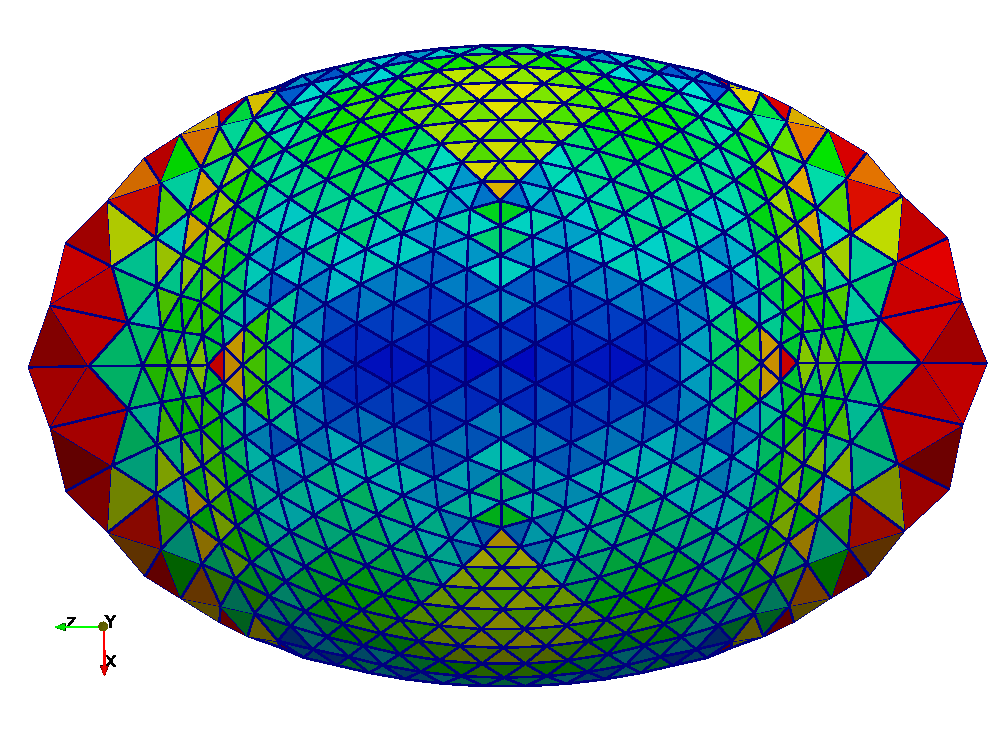
\includegraphics[width=0.45\textwidth]{videos/meshCorr/step0.eps}\hfill
                                                                   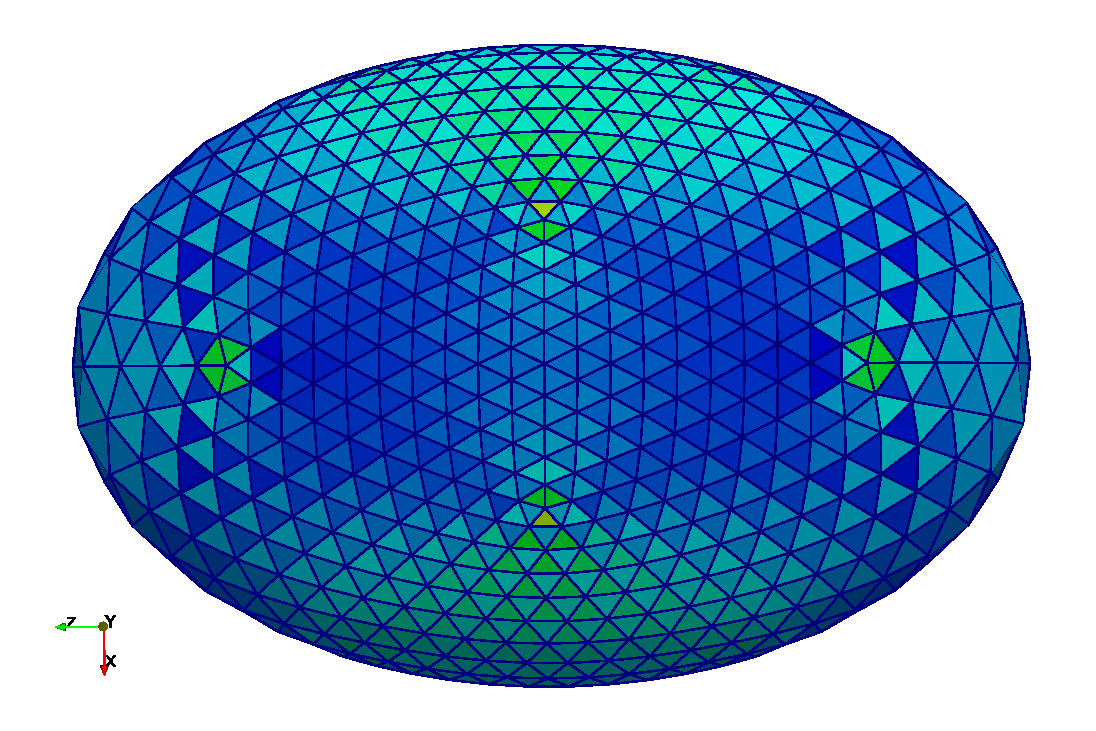
\includegraphics[width=0.49\textwidth]{videos/meshCorr/step1000.eps}\\
                                                                   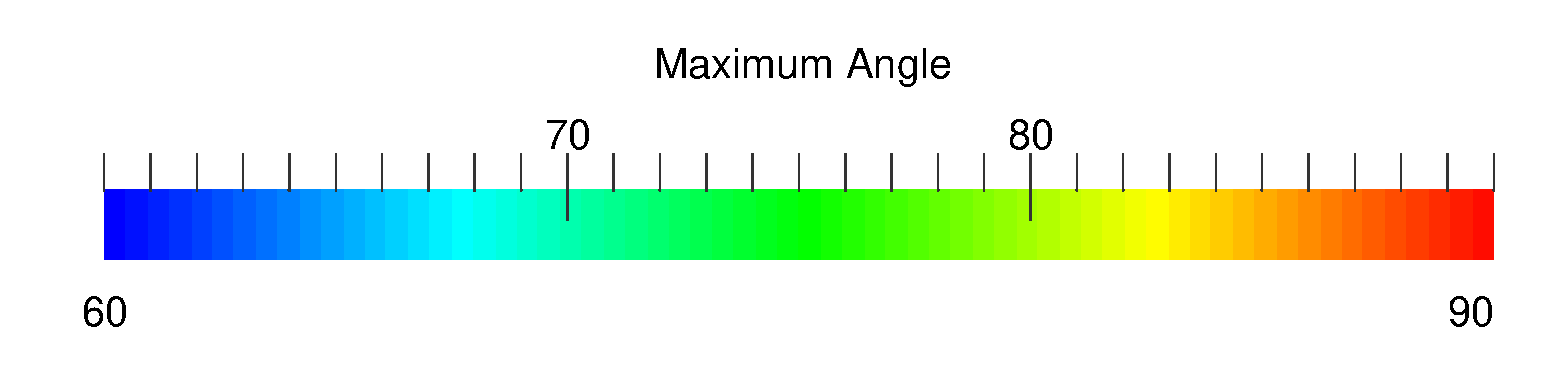
\includegraphics[width=0.6\textwidth]{videos/meshCorr/bar.eps}}
      \onslide<4> \centering\href{run:videos/meshCorr/runVideo.sh}{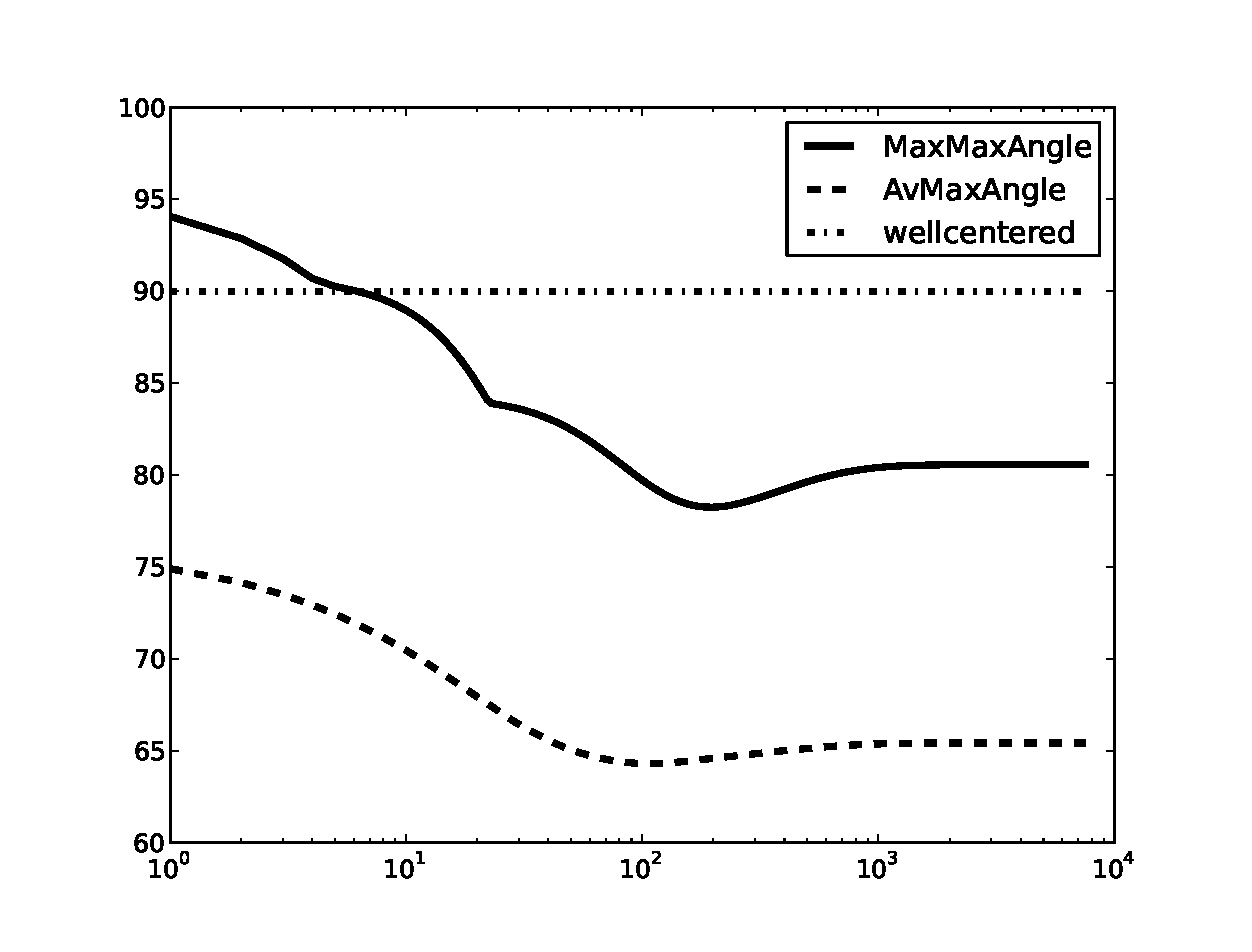
\includegraphics[width=0.6\textwidth]{videos/meshCorr/plot.eps}}
    \end{overprint}
  \end{frame}

  \begin{frame}
    \begin{block}{Dualgitter \( \csd K \)}
      Das Dualgitter \( \csd K \) ist die Umkreismittelpunktsunterteilung eines wohlzentrierten Primärgitters.
      Dazu gehören \( \ldots \) 
      \begin{itemize}
        \item<2-> alle Umkreismittelpunkte \( c(\sigma^{p}) \)
        \item<3-> alle Kanten \( s[c(\sigma^{p}), c(\sigma^{q})] \) mit \( \sigma^{p}\prec\sigma^{q} \)
        \item<4-> alle Dreiecke \( s[c(\sigma^{p}), c(\sigma^{q}),  c(\sigma^{r})] \) mit \( \sigma^{p}\prec\sigma^{q}\prec\sigma^{r} \)
      \end{itemize}
    \end{block}
      \begin{overprint}
        \onslide<1> \centering\begin{tikzpicture}[>=latex, line width=1pt]
  % Coords
  \coordinate (V0) at (2,0);
  \coordinate (V1) at (2,2);
  \coordinate (V2) at (0,1);
  \coordinate (V3) at (4,1);
  \coordinate (V4) at (4,-1);
  \coordinate (V5) at (0,-1);
 \coordinate (V6) at (2,-2);

\fill[opacity=0.4]  (V1) -- (V3) -- (V4) -- (V6) -- (V5) -- (V2);


  % Arrows\tilde{\sigma}
  \draw(V0) -- (V1);
  \draw(V1) --  (V2);
  \draw(V0) -- (V2);
  \draw(V1) --  (V3);
  \draw(V0) -- (V3);
   \draw(V0) -- (V4);
  \draw(V0) -- (V5);
  \draw(V5) --  (V2);
  \draw(V3) --  (V4);
 \draw(V4) -- (V6);
\draw(V0) -- (V6);
\draw(V6) -- (V5);
  % Points
  \fill (V0) circle (2pt);
  \fill (V1) circle (2pt);
  \fill (V2) circle (2pt);
  \fill (V3) circle (2pt);
  \fill (V4) circle (2pt);
  \fill (V5)circle (2pt);
 \fill (V6)circle (2pt);


\draw[opacity=0] (V5) -- (V4);
  %circumcenter
  %\coordinate (CC1) at (1.333,1);
  %\coordinate (CC0) at (2.666,1);
  %\coordinate (CC2) at (0.666,0);
  %\coordinate (CCm) at (3.333,0);
  %\coordinate (CCC0) at (2,1);
  %\coordinate (CCC1) at (1,0.5);
  %\coordinate (CCC2) at (3,0.5);
  %\coordinate (CCC3) at (1,-0.5);
  %\coordinate (CCC4) at (3,-0.5);
 % \fill (CC0) circle (2pt);
  %\fill (CC1) circle (2pt);
  %\fill (CC2) circle (2pt);
  %\fill (CCm) circle (2pt);
  %\fill (CCC0) circle (2pt);
  %\fill (CCC1) circle (2pt);
  %\fill (CCC2) circle (2pt);
  %\fill (CCC3) circle (2pt);
  %\fill (CCC4) circle (2pt);
  %\draw[line width=1pt, ->,style=dotted] (CC0) -- (CC1);
  %\draw[line width=1pt, ->,style=dotted] (CC1) -- (CC2);
 % \draw[line width=1pt, ->,style=dotted] (CCm) -- (CC0);
 % \draw[line width=1pt,style=dotted] (CC2) -- (CCC3);
 % \draw[line width=1pt,->,style=dotted] (CCC4) -- (CCm);

\end{tikzpicture}


        \onslide<2> \centering\begin{tikzpicture}[>=latex, line width=1pt]
  % Coords
  \coordinate (V0) at (2,0);
  \coordinate (V1) at (2,2);
  \coordinate (V2) at (0,1);
  \coordinate (V3) at (4,1);
  \coordinate (V4) at (4,-1);
  \coordinate (V5) at (0,-1);
 \coordinate (V6) at (2,-2);

\fill[opacity=0.4]  (V1) -- (V3) -- (V4) -- (V6) -- (V5) -- (V2);
  % Arrows\tilde{\sigma}
  \draw(V0) -- (V1);
  \draw(V1) --  (V2);
  \draw(V0) -- (V2);
  \draw(V1) --  (V3);
  \draw(V0) -- (V3);
   \draw(V0) -- (V4);
  \draw(V0) -- (V5);
  \draw(V5) --  (V2);
  \draw(V3) --  (V4);
 \draw(V4) -- (V6);
\draw(V0) -- (V6);
\draw(V6) -- (V5);
  % Points
  \fill[red] (V0) circle (2pt);
  \fill[red] (V1) circle (2pt);
  \fill[red] (V2) circle (2pt);
  \fill[red] (V3) circle (2pt);
  \fill[red] (V4) circle (2pt);
  \fill[red] (V5)circle (2pt);
 \fill[red] (V6)circle (2pt);



  %circumcenter
  \coordinate (CC1) at (1.333,1);
  \coordinate (CC0) at (2.666,1);
 \coordinate (CC3) at (1.333,-1);
  \coordinate (CC2) at (0.666,0);
\coordinate (CC4) at (2.666,-1);
  \coordinate (CC5) at (3.333,0);

  \fill[red] (CC0) circle (2pt);
  \fill[red] (CC1) circle (2pt);
  \fill[red] (CC2) circle (2pt);
 \fill[red] (CC3) circle (2pt);
 \fill[red] (CC4) circle (2pt);
  \fill[red] (CC5) circle (2pt);


  \coordinate (C01) at (2,1);
  \coordinate (C02) at (1,0.5);
  \coordinate (C03) at (3,0.5);
  \coordinate (C05) at (1,-0.5);
  \coordinate (C04) at (3,-0.5);
\coordinate (C06) at (2,-1);

  \fill[red] (C01) circle (2pt);
  \fill[red] (C02) circle (2pt);
  \fill[red] (C03) circle (2pt);
  \fill[red] (C05) circle (2pt);
  \fill[red] (C04) circle (2pt);
\fill[red] (C06) circle (2pt);

\coordinate (C12) at (1,1.5);
\coordinate (C25) at (0,0);
\coordinate (C56) at (1,-1.5);
\coordinate (C46) at (3,-1.5);
\coordinate (C34) at (4,0);
\coordinate (C13) at (3,1.5);

\fill[red] (C12) circle (2pt);
\fill[red] (C25) circle (2pt);
\fill[red] (C56) circle (2pt);
\fill[red] (C46) circle (2pt);
\fill[red] (C34) circle (2pt);
\fill[red] (C13) circle (2pt);
  %\draw[line width=1pt, ->,style=dotted] (CC0) -- (CC1);
  %\draw[line width=1pt, ->,style=dotted] (CC1) -- (CC2);
 % \draw[line width=1pt, ->,style=dotted] (CCm) -- (CC0);
 % \draw[line width=1pt,style=dotted] (CC2) -- (CCC3);
 % \draw[line width=1pt,->,style=dotted] (CCC4) -- (CCm);

\end{tikzpicture}


        \onslide<3> \centering\begin{tikzpicture}[>=latex, line width=1pt]
  % Coords
  \coordinate (V0) at (2,0);
  \coordinate (V1) at (2,2);
  \coordinate (V2) at (0,1);
  \coordinate (V3) at (4,1);
  \coordinate (V4) at (4,-1);
  \coordinate (V5) at (0,-1);
 \coordinate (V6) at (2,-2);

%circumcenter
  \coordinate (CC1) at (1.333,1);
  \coordinate (CC0) at (2.666,1);
 \coordinate (CC3) at (1.333,-1);
  \coordinate (CC2) at (0.666,0);
\coordinate (CC4) at (2.666,-1);
  \coordinate (CC5) at (3.333,0);

 
  \coordinate (C01) at (2,1);
  \coordinate (C02) at (1,0.5);
  \coordinate (C03) at (3,0.5);
  \coordinate (C05) at (1,-0.5);
  \coordinate (C04) at (3,-0.5);
\coordinate (C06) at (2,-1);

\coordinate (C12) at (1,1.5);
\coordinate (C25) at (0,0);
\coordinate (C56) at (1,-1.5);
\coordinate (C46) at (3,-1.5);
\coordinate (C34) at (4,0);
\coordinate (C13) at (3,1.5);

\fill[opacity=0.4]  (V1) -- (V3) -- (V4) -- (V6) -- (V5) -- (V2);
  % Arrows\tilde{\sigma}
  \draw[red](V0) -- (V1);
  \draw[red](V1) --  (V2);
  \draw[red](V0) -- (V2);
  \draw[red](V1) --  (V3);
  \draw[red](V0) -- (V3);
   \draw[red](V0) -- (V4);
  \draw[red](V0) -- (V5);
  \draw[red](V5) --  (V2);
  \draw[red](V3) --  (V4);
 \draw[red](V4) -- (V6);
\draw[red](V0) -- (V6);
\draw[red](V6) -- (V5);
 
\draw[red] (CC0) -- (CC1) -- (CC2) -- (CC3) -- (CC4) -- (CC5) -- (CC0);
\draw[red] (C12) -- (CC1);
\draw[red] (C25) -- (CC2);
\draw[red] (C56) -- (CC3);
\draw[red] (C46) -- (CC4);
\draw[red] (C34) -- (CC5);
\draw[red] (C13) -- (CC0);
\draw[red, dotted] (CC1) -- (CC4);
\draw[red, dotted] (CC2) -- (CC5);
\draw[red, dotted] (CC3) -- (CC0);

\draw[red, dotted] (CC1) -- (V1);
\draw[red, dotted] (CC2) -- (V2);
\draw[red, dotted] (CC3) -- (V5);
\draw[red, dotted] (CC4) -- (V6);
\draw[red, dotted] (CC5) -- (V4);
\draw[red, dotted] (CC0) -- (V3);

\draw[red, dotted] (CC1) -- (V2);
\draw[red, dotted] (CC2) -- (V5);
\draw[red, dotted] (CC3) -- (V6);
\draw[red, dotted] (CC4) -- (V4);
\draw[red, dotted] (CC5) -- (V3);
\draw[red, dotted] (CC0) -- (V1);

  

 \fill (V0) circle (2pt);
  \fill (V1) circle (2pt);
  \fill (V2) circle (2pt);
  \fill (V3) circle (2pt);
  \fill (V4) circle (2pt);
  \fill (V5)circle (2pt);
 \fill (V6)circle (2pt);

 \fill (CC0) circle (2pt);
  \fill (CC1) circle (2pt);
  \fill (CC2) circle (2pt);
 \fill (CC3) circle (2pt);
 \fill (CC4) circle (2pt);
  \fill (CC5) circle (2pt);



  \fill (C01) circle (2pt);
  \fill (C02) circle (2pt);
  \fill (C03) circle (2pt);
  \fill (C05) circle (2pt);
  \fill (C04) circle (2pt);
\fill (C06) circle (2pt);
 

\fill (C12) circle (2pt);
\fill (C25) circle (2pt);
\fill (C56) circle (2pt);
\fill (C46) circle (2pt);
\fill (C34) circle (2pt);
\fill (C13) circle (2pt);


\end{tikzpicture}


        \onslide<4> \centering\begin{tikzpicture}[>=latex, line width=1pt]
  % Coords
  \coordinate (V0) at (2,0);
  \coordinate (V1) at (2,2);
  \coordinate (V2) at (0,1);
  \coordinate (V3) at (4,1);
  \coordinate (V4) at (4,-1);
  \coordinate (V5) at (0,-1);
 \coordinate (V6) at (2,-2);

%circumcenter
  \coordinate (CC1) at (1.333,1);
  \coordinate (CC0) at (2.666,1);
 \coordinate (CC3) at (1.333,-1);
  \coordinate (CC2) at (0.666,0);
\coordinate (CC4) at (2.666,-1);
  \coordinate (CC5) at (3.333,0);

 
  \coordinate (C01) at (2,1);
  \coordinate (C02) at (1,0.5);
  \coordinate (C03) at (3,0.5);
  \coordinate (C05) at (1,-0.5);
  \coordinate (C04) at (3,-0.5);
\coordinate (C06) at (2,-1);

\coordinate (C12) at (1,1.5);
\coordinate (C25) at (0,0);
\coordinate (C56) at (1,-1.5);
\coordinate (C46) at (3,-1.5);
\coordinate (C34) at (4,0);
\coordinate (C13) at (3,1.5);

\fill[opacity=1, red]  (V1) -- (V3) -- (V4) -- (V6) -- (V5) -- (V2);
  % Arrows\tilde{\sigma}
  \draw(V0) -- (V1);
  \draw(V1) --  (V2);
  \draw(V0) -- (V2);
  \draw(V1) --  (V3);
  \draw(V0) -- (V3);
   \draw(V0) -- (V4);
  \draw(V0) -- (V5);
  \draw(V5) --  (V2);
  \draw(V3) --  (V4);
 \draw(V4) -- (V6);
\draw(V0) -- (V6);
\draw(V6) -- (V5);
 
\draw (CC0) -- (CC1) -- (CC2) -- (CC3) -- (CC4) -- (CC5) -- (CC0);
\draw (C12) -- (CC1);
\draw (C25) -- (CC2);
\draw (C56) -- (CC3);
\draw (C46) -- (CC4);
\draw (C34) -- (CC5);
\draw (C13) -- (CC0);
\draw[dotted] (CC1) -- (CC4);
\draw[dotted] (CC2) -- (CC5);
\draw[dotted] (CC3) -- (CC0);

\draw[dotted] (CC1) -- (V1);
\draw[dotted] (CC2) -- (V2);
\draw[dotted] (CC3) -- (V5);
\draw[dotted] (CC4) -- (V6);
\draw[dotted] (CC5) -- (V4);
\draw[dotted] (CC0) -- (V3);

\draw[dotted] (CC1) -- (V2);
\draw[dotted] (CC2) -- (V5);
\draw[dotted] (CC3) -- (V6);
\draw[dotted] (CC4) -- (V4);
\draw[dotted] (CC5) -- (V3);
\draw[dotted] (CC0) -- (V1);

  

 \fill (V0) circle (2pt);
  \fill (V1) circle (2pt);
  \fill (V2) circle (2pt);
  \fill (V3) circle (2pt);
  \fill (V4) circle (2pt);
  \fill (V5)circle (2pt);
 \fill (V6)circle (2pt);

 \fill (CC0) circle (2pt);
  \fill (CC1) circle (2pt);
  \fill (CC2) circle (2pt);
 \fill (CC3) circle (2pt);
 \fill (CC4) circle (2pt);
  \fill (CC5) circle (2pt);



  \fill (C01) circle (2pt);
  \fill (C02) circle (2pt);
  \fill (C03) circle (2pt);
  \fill (C05) circle (2pt);
  \fill (C04) circle (2pt);
\fill (C06) circle (2pt);
 

\fill (C12) circle (2pt);
\fill (C25) circle (2pt);
\fill (C56) circle (2pt);
\fill (C46) circle (2pt);
\fill (C34) circle (2pt);
\fill (C13) circle (2pt);


\end{tikzpicture}


        \onslide<5> \centering\begin{tikzpicture}[>=latex, line width=1pt]
  % Coords
  \coordinate (V0) at (2,0);
  \coordinate (V1) at (2,2);
  \coordinate (V2) at (0,1);
  \coordinate (V3) at (4,1);
  \coordinate (V4) at (4,-1);
  \coordinate (V5) at (0,-1);
 \coordinate (V6) at (2,-2);

%circumcenter
  \coordinate (CC1) at (1.333,1);
  \coordinate (CC0) at (2.666,1);
 \coordinate (CC3) at (1.333,-1);
  \coordinate (CC2) at (0.666,0);
\coordinate (CC4) at (2.666,-1);
  \coordinate (CC5) at (3.333,0);

 
  \coordinate (C01) at (2,1);
  \coordinate (C02) at (1,0.5);
  \coordinate (C03) at (3,0.5);
  \coordinate (C05) at (1,-0.5);
  \coordinate (C04) at (3,-0.5);
\coordinate (C06) at (2,-1);

\coordinate (C12) at (1,1.5);
\coordinate (C25) at (0,0);
\coordinate (C56) at (1,-1.5);
\coordinate (C46) at (3,-1.5);
\coordinate (C34) at (4,0);
\coordinate (C13) at (3,1.5);

%\fill[opacity=0.4]  (V1) -- (V3) -- (V4) -- (V6) -- (V5) -- (V2);
  % Arrows\tilde{\sigma}
  \draw[dotted](V0) -- (V1);
  \draw[dotted](V1) --  (V2);
  \draw[dotted](V0) -- (V2);
  \draw[dotted](V1) --  (V3);
  \draw[dotted](V0) -- (V3);
   \draw[dotted](V0) -- (V4);
  \draw[dotted](V0) -- (V5);
  \draw[dotted](V5) --  (V2);
  \draw[dotted](V3) --  (V4);
 \draw[dotted](V4) -- (V6);
\draw[dotted](V0) -- (V6);
\draw[dotted](V6) -- (V5);
 
\draw (CC0) -- (CC1) -- (CC2) -- (CC3) -- (CC4) -- (CC5) -- (CC0);
\draw (C12) -- (CC1);
\draw (C25) -- (CC2);
\draw (C56) -- (CC3);
\draw (C46) -- (CC4);
\draw (C34) -- (CC5);
\draw (C13) -- (CC0);
\draw[dotted] (CC1) -- (CC4);
\draw[dotted] (CC2) -- (CC5);
\draw[dotted] (CC3) -- (CC0);

\draw[dotted] (CC1) -- (V1);
\draw[dotted] (CC2) -- (V2);
\draw[dotted] (CC3) -- (V5);
\draw[dotted] (CC4) -- (V6);
\draw[dotted] (CC5) -- (V4);
\draw[dotted] (CC0) -- (V3);

\draw[dotted] (CC1) -- (V2);
\draw[dotted] (CC2) -- (V5);
\draw[dotted] (CC3) -- (V6);
\draw[dotted] (CC4) -- (V4);
\draw[dotted] (CC5) -- (V3);
\draw[dotted] (CC0) -- (V1);

  

 \fill (V0) circle (2pt);
  \fill (V1) circle (2pt);
  \fill (V2) circle (2pt);
  \fill (V3) circle (2pt);
  \fill (V4) circle (2pt);
  \fill (V5)circle (2pt);
 \fill (V6)circle (2pt);

 \fill (CC0) circle (2pt);
  \fill (CC1) circle (2pt);
  \fill (CC2) circle (2pt);
 \fill (CC3) circle (2pt);
 \fill (CC4) circle (2pt);
  \fill (CC5) circle (2pt);



  \fill (C01) circle (2pt);
  \fill (C02) circle (2pt);
  \fill (C03) circle (2pt);
  \fill (C05) circle (2pt);
  \fill (C04) circle (2pt);
\fill (C06) circle (2pt);
 

\fill (C12) circle (2pt);
\fill (C25) circle (2pt);
\fill (C56) circle (2pt);
\fill (C46) circle (2pt);
\fill (C34) circle (2pt);
\fill (C13) circle (2pt);


\end{tikzpicture}


      \end{overprint}
      \visible<5->{Das Dualgitter ist wieder ein Primärgitter, aber kein wohlzentriertes.}
  \end{frame}

  \begin{frame}
  \small
    \begin{block}{Kettenkomplex \( C_{p}(K) \)}
      \begin{itemize}
        \setlength{\itemsep}{1pt}
        \item<1->  Eine \( p \)-Kette aus \( C_{p}(K) \) ist eine formale Summe aus \( p \)-Simplizes
            \begin{align*}
              C_{p}(K) &:= \left\{\sum_{\sigma\in K^{(p)}}a_{\sigma}\sigma \middle| a_{\sigma}\in\Z \right\}
            \end{align*}
        \item<2-> zB. \( c^{1} := \sigma^{1}_{0} - \sigma^{1}_{1} + 2\sigma^{1}_{2}\in C_{1}(K) \)
        \item<3-> zB. \( c^{2} := \sum_{\sigma^{2}\succ v} \sigma^{2} \in C_{2}(\csd K) \) (1-Ring um \( v \) im \( \csd K \), \( \star v \))
      \end{itemize}
    \end{block}
      \begin{overprint}
        \onslide<2> \centering\begin{tikzpicture}[>=latex, line width=1pt, scale=0.9]
  % Coords
  \coordinate (V0) at (2,0);
  \coordinate (V1) at (2,2);
  \coordinate (V2) at (0,1);
  \coordinate (V3) at (4,1);
  \coordinate (V4) at (4,-1);
  \coordinate (V5) at (0,-1);
 \coordinate (V6) at (2,-2);


\fill[opacity=0.4]  (V1) -- (V3) -- (V4) -- (V6) -- (V5) -- (V2);


  % Arrows\tilde{\sigma}
  \draw[red,->](V1) --node[left, black]{\(\sigma^1_0\)} node[right, black]{\small 1} (V0);
  \draw(V1) --  (V2);
  \draw(V0) -- (V2);
  \draw(V1) --  (V3);
  \draw(V0) -- (V3);
   \draw(V0) -- (V4);
  \draw[red,->](V0) --node[above left=-3pt, black]{\(\sigma^1_1\)} node[below right=-3pt, black]{\small -1} (V5);
  \draw(V5) --  (V2);
  \draw(V3) --  (V4);
 \draw(V4) -- (V6);
\draw(V0) -- (V6);
\draw[red,->](V5)  --node[below left=-3pt, black]{\(\sigma^1_2\)} node[above right=-3pt, black]{\small 2}(V6);
  % Points
  \fill (V0) circle (2pt);
  \fill (V1) circle (2pt);
  \fill (V2) circle (2pt);
  \fill (V3) circle (2pt);
  \fill (V4) circle (2pt);
  \fill (V5)circle (2pt);
 \fill (V6)circle (2pt);



\end{tikzpicture}


        \onslide<3> \centering\begin{tikzpicture}[>=latex, line width=1pt, scale=0.9]
  % Coords
  \coordinate (V0) at (2,0);
  \coordinate (V1) at (2,2);
  \coordinate (V2) at (0,1);
  \coordinate (V3) at (4,1);
  \coordinate (V4) at (4,-1);
  \coordinate (V5) at (0,-1);
 \coordinate (V6) at (2,-2);

%circumcenter
  \coordinate (CC1) at (1.333,1);
  \coordinate (CC0) at (2.666,1);
 \coordinate (CC3) at (1.333,-1);
  \coordinate (CC2) at (0.666,0);
\coordinate (CC4) at (2.666,-1);
  \coordinate (CC5) at (3.333,0);

 
  \coordinate (C01) at (2,1);
  \coordinate (C02) at (1,0.5);
  \coordinate (C03) at (3,0.5);
  \coordinate (C05) at (1,-0.5);
  \coordinate (C04) at (3,-0.5);
\coordinate (C06) at (2,-1);

\coordinate (C12) at (1,1.5);
\coordinate (C25) at (0,0);
\coordinate (C56) at (1,-1.5);
\coordinate (C46) at (3,-1.5);
\coordinate (C34) at (4,0);
\coordinate (C13) at (3,1.5);

\fill[opacity=0.4]  (V1) -- (V3) -- (V4) -- (V6) -- (V5) -- (V2);
\fill[red] (CC0) -- (CC1) -- (CC2) -- (CC3) -- (CC4) -- (CC5);
  % Arrows\tilde{\sigma}
  \draw(V0) -- (V1);
  \draw(V1) --  (V2);
  \draw(V0) -- (V2);
  \draw(V1) --  (V3);
  \draw(V0) -- (V3);
   \draw(V0) -- (V4);
  \draw(V0) -- (V5);
  \draw(V5) --  (V2);
  \draw(V3) --  (V4);
 \draw(V4) -- (V6);
\draw(V0) -- (V6);
\draw(V6) -- (V5);
 
\draw (CC0) -- (CC1) -- (CC2) -- (CC3) -- (CC4) -- (CC5) -- (CC0);
\draw (C12) -- (CC1);
\draw (C25) -- (CC2);
\draw (C56) -- (CC3);
\draw (C46) -- (CC4);
\draw (C34) -- (CC5);
\draw (C13) -- (CC0);
\draw[dotted] (CC1) -- (CC4);
\draw[dotted] (CC2) -- (CC5);
\draw[dotted] (CC3) -- (CC0);

\draw[dotted] (CC1) -- (V1);
\draw[dotted] (CC2) -- (V2);
\draw[dotted] (CC3) -- (V5);
\draw[dotted] (CC4) -- (V6);
\draw[dotted] (CC5) -- (V4);
\draw[dotted] (CC0) -- (V3);

\draw[dotted] (CC1) -- (V2);
\draw[dotted] (CC2) -- (V5);
\draw[dotted] (CC3) -- (V6);
\draw[dotted] (CC4) -- (V4);
\draw[dotted] (CC5) -- (V3);
\draw[dotted] (CC0) -- (V1);

  

 \fill (V0)node[above]{\Large\textit v \phantom{l}} circle (3pt);
  \fill (V1) circle (2pt);
  \fill (V2) circle (2pt);
  \fill (V3) circle (2pt);
  \fill (V4) circle (2pt);
  \fill (V5)circle (2pt);
 \fill (V6)circle (2pt);

 \fill (CC0) circle (2pt);
  \fill (CC1) circle (2pt);
  \fill (CC2) circle (2pt);
 \fill (CC3) circle (2pt);
 \fill (CC4) circle (2pt);
  \fill (CC5) circle (2pt);



  \fill (C01) circle (2pt);
  \fill (C02) circle (2pt);
  \fill (C03) circle (2pt);
  \fill (C05) circle (2pt);
  \fill (C04) circle (2pt);
\fill (C06) circle (2pt);
 

\fill (C12) circle (2pt);
\fill (C25) circle (2pt);
\fill (C56) circle (2pt);
\fill (C46) circle (2pt);
\fill (C34) circle (2pt);
\fill (C13) circle (2pt);


\end{tikzpicture}


      \end{overprint}
  \end{frame}

  \begin{frame}
    \begin{block}{Sternoperator \( \star: C_{p}(K) \rightarrow   C_{n-p}(\star K) < C_{n-p}(\csd K) \)}
      \begin{align*}
       \star\sigma^{p} := \sum_{\sigma^{p} \prec \sigma^{p+1} \prec \ldots \prec \sigma^{n}}
                                                   s_{\sigma^{p} \sigma^{p+1} \ldots \sigma^{n}} \left[ c(\sigma^{p}), c(\sigma^{p+1}), \ldots, c(\sigma^{n}) \right]
      \end{align*}
      \begin{itemize}
        \item<2-> Knoten \( \sigma^{0} \) \( \mapsto \) Voronoizelle \( \star\sigma^{0}\in C_{2}(\star K) \)
        \item<3-> Kante \( \sigma^{1} \) \( \mapsto \) Voronoikante \( \star\sigma^{1}\in C_{1}(\star K) \)
        \item<4-> Dreieck \( \sigma^{2} \) \( \mapsto \) Voronoiknoten \( \star\sigma^{2}\in C_{0}(\star K) \)
      \end{itemize}
    \end{block}
    \begin{overprint}
      \onslide<2> 
        \begin{minipage}{0.4\textwidth}
          \centering\begin{tikzpicture}[>=latex, line width=1pt, scale=0.9]
  % Coords
  \coordinate (V0) at (2,0);
  \coordinate (V1) at (2,2);
  \coordinate (V2) at (0,1);
  \coordinate (V3) at (4,1);
  \coordinate (V4) at (4,-1);
  \coordinate (V5) at (0,-1);
 \coordinate (V6) at (2,-2);

%circumcenter
  \coordinate (CC1) at (1.333,1);
  \coordinate (CC0) at (2.666,1);
 \coordinate (CC3) at (1.333,-1);
  \coordinate (CC2) at (0.666,0);
\coordinate (CC4) at (2.666,-1);
  \coordinate (CC5) at (3.333,0);

 
  \coordinate (C01) at (2,1);
  \coordinate (C02) at (1,0.5);
  \coordinate (C03) at (3,0.5);
  \coordinate (C05) at (1,-0.5);
  \coordinate (C04) at (3,-0.5);
\coordinate (C06) at (2,-1);

\coordinate (C12) at (1,1.5);
\coordinate (C25) at (0,0);
\coordinate (C56) at (1,-1.5);
\coordinate (C46) at (3,-1.5);
\coordinate (C34) at (4,0);
\coordinate (C13) at (3,1.5);

\fill[opacity=0.4]  (V1) -- (V3) -- (V4) -- (V6) -- (V5) -- (V2);
%\fill[red] (CC0) -- (CC1) -- (CC2) -- (CC3) -- (CC4) -- (CC5);
  % Arrows\tilde{\sigma}
  \draw(V0) -- (V1);
  \draw(V1) --  (V2);
  \draw(V0) -- (V2);
  \draw(V1) --  (V3);
  \draw(V0) -- (V3);
   \draw(V0) -- (V4);
  \draw(V0) -- (V5);
  \draw(V5) --  (V2);
  \draw(V3) --  (V4);
 \draw(V4) -- (V6);
\draw(V0) -- (V6);
\draw(V6) -- (V5);
 
%\draw (CC0) -- (CC1) -- (CC2) -- (CC3) -- (CC4) -- (CC5) -- (CC0);
%\draw (C12) -- (CC1);
%\draw (C25) -- (CC2);
%\draw (C56) -- (CC3);
%\draw (C46) -- (CC4);
%\draw (C34) -- (CC5);
%\draw (C13) -- (CC0);
%\draw[dotted] (CC1) -- (CC4);
%\draw[dotted] (CC2) -- (CC5);
%\draw[dotted] (CC3) -- (CC0);

%\draw[dotted] (CC1) -- (V1);
%\draw[dotted] (CC2) -- (V2);
%\draw[dotted] (CC3) -- (V5);
%\draw[dotted] (CC4) -- (V6);
%\draw[dotted] (CC5) -- (V4);
%\draw[dotted] (CC0) -- (V3);

%\draw[dotted] (CC1) -- (V2);
%\draw[dotted] (CC2) -- (V5);
%\draw[dotted] (CC3) -- (V6);
%\draw[dotted] (CC4) -- (V4);
%\draw[dotted] (CC5) -- (V3);
%\draw[dotted] (CC0) -- (V1);

  

 \fill (V0) circle (3pt)[red];
  \fill (V1) circle (2pt);
  \fill (V2) circle (2pt);
  \fill (V3) circle (2pt);
  \fill (V4) circle (2pt);
  \fill (V5)circle (2pt);
 \fill (V6)circle (2pt);

% \fill (CC0) circle (2pt);
 %\fill (CC1) circle (2pt);
 %\fill (CC2) circle (2pt);
%\fill (CC3) circle (2pt);
%\fill (CC4) circle (2pt);
 %\fill (CC5) circle (2pt);



 %\fill (C01) circle (2pt);
 %\fill (C02) circle (2pt);
 %\fill (C03) circle (2pt);
 %\fill (C05) circle (2pt);
 %\fill (C04) circle (2pt);
%\fill (C06) circle (2pt);
 

%\fill (C12) circle (2pt);
%\fill (C25) circle (2pt);
%\fill (C56) circle (2pt);
%\fill (C46) circle (2pt);
%\fill (C34) circle (2pt);
%\fill (C13) circle (2pt);


\end{tikzpicture}

 
        \end{minipage}\hfill
       {\Huge\(\longmapsto\)}  \hfill
       \begin{minipage}{0.4\textwidth}
          \centering\begin{tikzpicture}[>=latex, line width=1pt, scale=0.9]
  % Coords
  \coordinate (V0) at (2,0);
  \coordinate (V1) at (2,2);
  \coordinate (V2) at (0,1);
  \coordinate (V3) at (4,1);
  \coordinate (V4) at (4,-1);
  \coordinate (V5) at (0,-1);
 \coordinate (V6) at (2,-2);

%circumcenter
  \coordinate (CC1) at (1.333,1);
  \coordinate (CC0) at (2.666,1);
 \coordinate (CC3) at (1.333,-1);
  \coordinate (CC2) at (0.666,0);
\coordinate (CC4) at (2.666,-1);
  \coordinate (CC5) at (3.333,0);

 
  \coordinate (C01) at (2,1);
  \coordinate (C02) at (1,0.5);
  \coordinate (C03) at (3,0.5);
  \coordinate (C05) at (1,-0.5);
  \coordinate (C04) at (3,-0.5);
\coordinate (C06) at (2,-1);

\coordinate (C12) at (1,1.5);
\coordinate (C25) at (0,0);
\coordinate (C56) at (1,-1.5);
\coordinate (C46) at (3,-1.5);
\coordinate (C34) at (4,0);
\coordinate (C13) at (3,1.5);

\fill[opacity=0.4]  (V1) -- (V3) -- (V4) -- (V6) -- (V5) -- (V2);
\fill[red] (CC0) -- (CC1) -- (CC2) -- (CC3) -- (CC4) -- (CC5);
  % Arrows\tilde{\sigma}
  \draw(V0) -- (V1);
  \draw(V1) --  (V2);
  \draw(V0) -- (V2);
  \draw(V1) --  (V3);
  \draw(V0) -- (V3);
   \draw(V0) -- (V4);
  \draw(V0) -- (V5);
  \draw(V5) --  (V2);
  \draw(V3) --  (V4);
 \draw(V4) -- (V6);
\draw(V0) -- (V6);
\draw(V6) -- (V5);
 
\draw (CC0) -- (CC1) -- (CC2) -- (CC3) -- (CC4) -- (CC5) -- (CC0);
%\draw (C12) -- (CC1);
%\draw (C25) -- (CC2);
%\draw (C56) -- (CC3);
%\draw (C46) -- (CC4);
%\draw (C34) -- (CC5);
%\draw (C13) -- (CC0);
\draw[dotted] (CC1) -- (CC4);
\draw[dotted] (CC2) -- (CC5);
\draw[dotted] (CC3) -- (CC0);

%\draw[dotted] (CC1) -- (V1);
%\draw[dotted] (CC2) -- (V2);
%\draw[dotted] (CC3) -- (V5);
%\draw[dotted] (CC4) -- (V6);
%\draw[dotted] (CC5) -- (V4);
%\draw[dotted] (CC0) -- (V3);

%\draw[dotted] (CC1) -- (V2);
%\draw[dotted] (CC2) -- (V5);
%\draw[dotted] (CC3) -- (V6);
%\draw[dotted] (CC4) -- (V4);
%\draw[dotted] (CC5) -- (V3);
%\draw[dotted] (CC0) -- (V1);

  

 \fill (V0) circle (3pt);
  \fill (V1) circle (2pt);
  \fill (V2) circle (2pt);
  \fill (V3) circle (2pt);
  \fill (V4) circle (2pt);
  \fill (V5)circle (2pt);
 \fill (V6)circle (2pt);

 \fill (CC0) circle (2pt);
  \fill (CC1) circle (2pt);
  \fill (CC2) circle (2pt);
 \fill (CC3) circle (2pt);
 \fill (CC4) circle (2pt);
  \fill (CC5) circle (2pt);



  \fill (C01) circle (2pt);
  \fill (C02) circle (2pt);
  \fill (C03) circle (2pt);
  \fill (C05) circle (2pt);
  \fill (C04) circle (2pt);
\fill (C06) circle (2pt);
 

%\fill (C12) circle (2pt);
%\fill (C25) circle (2pt);
%\fill (C56) circle (2pt);
%\fill (C46) circle (2pt);
%\fill (C34) circle (2pt);
%\fill (C13) circle (2pt);


\end{tikzpicture}

 
        \end{minipage}
      \onslide<3> 
        \begin{minipage}{0.4\textwidth}
          \centering\begin{tikzpicture}[>=latex, line width=1pt, scale=0.9]
  % Coords
  \coordinate (V0) at (2,0);
  \coordinate (V1) at (2,2);
  \coordinate (V2) at (0,1);
  \coordinate (V3) at (4,1);
  \coordinate (V4) at (4,-1);
  \coordinate (V5) at (0,-1);
 \coordinate (V6) at (2,-2);

%circumcenter
  \coordinate (CC1) at (1.333,1);
  \coordinate (CC0) at (2.666,1);
 \coordinate (CC3) at (1.333,-1);
  \coordinate (CC2) at (0.666,0);
\coordinate (CC4) at (2.666,-1);
  \coordinate (CC5) at (3.333,0);

 
  \coordinate (C01) at (2,1);
  \coordinate (C02) at (1,0.5);
  \coordinate (C03) at (3,0.5);
  \coordinate (C05) at (1,-0.5);
  \coordinate (C04) at (3,-0.5);
\coordinate (C06) at (2,-1);

\coordinate (C12) at (1,1.5);
\coordinate (C25) at (0,0);
\coordinate (C56) at (1,-1.5);
\coordinate (C46) at (3,-1.5);
\coordinate (C34) at (4,0);
\coordinate (C13) at (3,1.5);

\fill[opacity=0.4]  (V1) -- (V3) -- (V4) -- (V6) -- (V5) -- (V2);
%\fill[red] (CC0) -- (CC1) -- (CC2) -- (CC3) -- (CC4) -- (CC5);
  % Arrows\tilde{\sigma}
  \draw[red,->](V0) -- (V1);
  \draw(V1) --  (V2);
  \draw(V0) -- (V2);
  \draw(V1) --  (V3);
  \draw(V0) -- (V3);
   \draw(V0) -- (V4);
  \draw(V0) -- (V5);
  \draw(V5) --  (V2);
  \draw(V3) --  (V4);
 \draw(V4) -- (V6);
\draw(V0) -- (V6);
\draw(V6) -- (V5);
 
%\draw (CC0) -- (CC1) -- (CC2) -- (CC3) -- (CC4) -- (CC5) -- (CC0);
%\draw (C12) -- (CC1);
%\draw (C25) -- (CC2);
%\draw (C56) -- (CC3);
%\draw (C46) -- (CC4);
%\draw (C34) -- (CC5);
%\draw (C13) -- (CC0);
%\draw[dotted] (CC1) -- (CC4);
%\draw[dotted] (CC2) -- (CC5);
%\draw[dotted] (CC3) -- (CC0);

%\draw[dotted] (CC1) -- (V1);
%\draw[dotted] (CC2) -- (V2);
%\draw[dotted] (CC3) -- (V5);
%\draw[dotted] (CC4) -- (V6);
%\draw[dotted] (CC5) -- (V4);
%\draw[dotted] (CC0) -- (V3);

%\draw[dotted] (CC1) -- (V2);
%\draw[dotted] (CC2) -- (V5);
%\draw[dotted] (CC3) -- (V6);
%\draw[dotted] (CC4) -- (V4);
%\draw[dotted] (CC5) -- (V3);
%\draw[dotted] (CC0) -- (V1);

  

 \fill (V0) circle (2pt);
  \fill (V1) circle (2pt);
  \fill (V2) circle (2pt);
  \fill (V3) circle (2pt);
  \fill (V4) circle (2pt);
  \fill (V5)circle (2pt);
 \fill (V6)circle (2pt);

% \fill (CC0) circle (2pt);
 %\fill (CC1) circle (2pt);
 %\fill (CC2) circle (2pt);
%\fill (CC3) circle (2pt);
%\fill (CC4) circle (2pt);
 %\fill (CC5) circle (2pt);



 %\fill (C01) circle (2pt);
 %\fill (C02) circle (2pt);
 %\fill (C03) circle (2pt);
 %\fill (C05) circle (2pt);
 %\fill (C04) circle (2pt);
%\fill (C06) circle (2pt);
 

%\fill (C12) circle (2pt);
%\fill (C25) circle (2pt);
%\fill (C56) circle (2pt);
%\fill (C46) circle (2pt);
%\fill (C34) circle (2pt);
%\fill (C13) circle (2pt);


\end{tikzpicture}

 
        \end{minipage}\hfill
       {\Huge\(\longmapsto\)}  \hfill
       \begin{minipage}{0.4\textwidth}
          \centering\begin{tikzpicture}[>=latex, line width=1pt, scale=0.9]
  % Coords
  \coordinate (V0) at (2,0);
  \coordinate (V1) at (2,2);
  \coordinate (V2) at (0,1);
  \coordinate (V3) at (4,1);
  \coordinate (V4) at (4,-1);
  \coordinate (V5) at (0,-1);
 \coordinate (V6) at (2,-2);

%circumcenter
  \coordinate (CC1) at (1.333,1);
  \coordinate (CC0) at (2.666,1);
 \coordinate (CC3) at (1.333,-1);
  \coordinate (CC2) at (0.666,0);
\coordinate (CC4) at (2.666,-1);
  \coordinate (CC5) at (3.333,0);

 
  \coordinate (C01) at (2,1);
  \coordinate (C02) at (1,0.5);
  \coordinate (C03) at (3,0.5);
  \coordinate (C05) at (1,-0.5);
  \coordinate (C04) at (3,-0.5);
\coordinate (C06) at (2,-1);

\coordinate (C12) at (1,1.5);
\coordinate (C25) at (0,0);
\coordinate (C56) at (1,-1.5);
\coordinate (C46) at (3,-1.5);
\coordinate (C34) at (4,0);
\coordinate (C13) at (3,1.5);

\fill[opacity=0.4]  (V1) -- (V3) -- (V4) -- (V6) -- (V5) -- (V2);
%\fill[red] (CC0) -- (CC1) -- (CC2) -- (CC3) -- (CC4) -- (CC5);
  % Arrows\tilde{\sigma}
  \draw[->](V0) -- (V1);
  \draw(V1) --  (V2);
  \draw(V0) -- (V2);
  \draw(V1) --  (V3);
  \draw(V0) -- (V3);
   \draw(V0) -- (V4);
  \draw(V0) -- (V5);
  \draw(V5) --  (V2);
  \draw(V3) --  (V4);
 \draw(V4) -- (V6);
\draw(V0) -- (V6);
\draw(V6) -- (V5);
 
\draw[dotted] (CC0) -- (CC1) -- (CC2) -- (CC3) -- (CC4) -- (CC5) -- (CC0);
\draw[red,->] (CC0) -- (CC1);
%\draw (C12) -- (CC1);
%\draw (C25) -- (CC2);
%\draw (C56) -- (CC3);
%\draw (C46) -- (CC4);
%\draw (C34) -- (CC5);
%\draw (C13) -- (CC0);
\draw[dotted] (CC1) -- (CC4);
\draw[dotted] (CC2) -- (CC5);
\draw[dotted] (CC3) -- (CC0);

%\draw[dotted] (CC1) -- (V1);
%\draw[dotted] (CC2) -- (V2);
%\draw[dotted] (CC3) -- (V5);
%\draw[dotted] (CC4) -- (V6);
%\draw[dotted] (CC5) -- (V4);
%\draw[dotted] (CC0) -- (V3);

%\draw[dotted] (CC1) -- (V2);
%\draw[dotted] (CC2) -- (V5);
%\draw[dotted] (CC3) -- (V6);
%\draw[dotted] (CC4) -- (V4);
%\draw[dotted] (CC5) -- (V3);
%\draw[dotted] (CC0) -- (V1);

  

 \fill (V0) circle (2pt);
  \fill (V1) circle (2pt);
  \fill (V2) circle (2pt);
  \fill (V3) circle (2pt);
  \fill (V4) circle (2pt);
  \fill (V5)circle (2pt);
 \fill (V6)circle (2pt);

 \fill (CC0) circle (2pt);
 \fill (CC1) circle (2pt);
 %\fill (CC2) circle (2pt);
%\fill (CC3) circle (2pt);
%\fill (CC4) circle (2pt);
 %\fill (CC5) circle (2pt);



 \fill (C01) circle (2pt);
 %\fill (C02) circle (2pt);
 %\fill (C03) circle (2pt);
 %\fill (C05) circle (2pt);
 %\fill (C04) circle (2pt);
%\fill (C06) circle (2pt);
 

%\fill (C12) circle (2pt);
%\fill (C25) circle (2pt);
%\fill (C56) circle (2pt);
%\fill (C46) circle (2pt);
%\fill (C34) circle (2pt);
%\fill (C13) circle (2pt);


\end{tikzpicture}

 
        \end{minipage}
      \onslide<4> 
        \begin{minipage}{0.4\textwidth}
          \centering\begin{tikzpicture}[>=latex, line width=1pt, scale=0.9]
  % Coords
  \coordinate (V0) at (2,0);
  \coordinate (V1) at (2,2);
  \coordinate (V2) at (0,1);
  \coordinate (V3) at (4,1);
  \coordinate (V4) at (4,-1);
  \coordinate (V5) at (0,-1);
 \coordinate (V6) at (2,-2);

%circumcenter
  \coordinate (CC1) at (1.333,1);
  \coordinate (CC0) at (2.666,1);
 \coordinate (CC3) at (1.333,-1);
  \coordinate (CC2) at (0.666,0);
\coordinate (CC4) at (2.666,-1);
  \coordinate (CC5) at (3.333,0);

 
  \coordinate (C01) at (2,1);
  \coordinate (C02) at (1,0.5);
  \coordinate (C03) at (3,0.5);
  \coordinate (C05) at (1,-0.5);
  \coordinate (C04) at (3,-0.5);
\coordinate (C06) at (2,-1);

\coordinate (C12) at (1,1.5);
\coordinate (C25) at (0,0);
\coordinate (C56) at (1,-1.5);
\coordinate (C46) at (3,-1.5);
\coordinate (C34) at (4,0);
\coordinate (C13) at (3,1.5);

\fill[opacity=0.4]  (V1) -- (V3) -- (V4) -- (V6) -- (V5) -- (V2);
\fill[red] (V0) -- (V3) -- (V1);
%\fill[red] (CC0) -- (CC1) -- (CC2) -- (CC3) -- (CC4) -- (CC5);
  % Arrows\tilde{\sigma}
  \draw(V0) -- (V1);
  \draw(V1) --  (V2);
  \draw(V0) -- (V2);
  \draw(V1) --  (V3);
  \draw(V0) -- (V3);
   \draw(V0) -- (V4);
  \draw(V0) -- (V5);
  \draw(V5) --  (V2);
  \draw(V3) --  (V4);
 \draw(V4) -- (V6);
\draw(V0) -- (V6);
\draw(V6) -- (V5);
 
%\draw[dotted] (CC0) -- (CC1) -- (CC2) -- (CC3) -- (CC4) -- (CC5) -- (CC0);
%\draw (C12) -- (CC1);
%\draw (C25) -- (CC2);
%\draw (C56) -- (CC3);
%\draw (C46) -- (CC4);
%\draw (C34) -- (CC5);
%\draw (C13) -- (CC0);
%\draw[dotted] (CC1) -- (CC4);
%\draw[dotted] (CC2) -- (CC5);
%\draw[dotted] (CC3) -- (CC0);

%\draw[dotted] (CC1) -- (V1);
%\draw[dotted] (CC2) -- (V2);
%\draw[dotted] (CC3) -- (V5);
%\draw[dotted] (CC4) -- (V6);
%\draw[dotted] (CC5) -- (V4);
%\draw[dotted] (CC0) -- (V3);

%\draw[dotted] (CC1) -- (V2);
%\draw[dotted] (CC2) -- (V5);
%\draw[dotted] (CC3) -- (V6);
%\draw[dotted] (CC4) -- (V4);
%\draw[dotted] (CC5) -- (V3);
%\draw[dotted] (CC0) -- (V1);

  

 \fill (V0) circle (2pt);
  \fill (V1) circle (2pt);
  \fill (V2) circle (2pt);
  \fill (V3) circle (2pt);
  \fill (V4) circle (2pt);
  \fill (V5)circle (2pt);
 \fill (V6)circle (2pt);

% \fill (CC0) circle (2pt);
 %\fill (CC1) circle (2pt);
 %\fill (CC2) circle (2pt);
%\fill (CC3) circle (2pt);
%\fill (CC4) circle (2pt);
 %\fill (CC5) circle (2pt);



% \fill (C01) circle (2pt);
 %\fill (C02) circle (2pt);
 %\fill (C03) circle (2pt);
 %\fill (C05) circle (2pt);
 %\fill (C04) circle (2pt);
%\fill (C06) circle (2pt);
 

%\fill (C12) circle (2pt);
%\fill (C25) circle (2pt);
%\fill (C56) circle (2pt);
%\fill (C46) circle (2pt);
%\fill (C34) circle (2pt);
%\fill (C13) circle (2pt);


\end{tikzpicture}

 
        \end{minipage}\hfill
       {\Huge\(\longmapsto\)}  \hfill
       \begin{minipage}{0.4\textwidth}
          \centering\begin{tikzpicture}[>=latex, line width=1pt, scale=0.9]
  % Coords
  \coordinate (V0) at (2,0);
  \coordinate (V1) at (2,2);
  \coordinate (V2) at (0,1);
  \coordinate (V3) at (4,1);
  \coordinate (V4) at (4,-1);
  \coordinate (V5) at (0,-1);
 \coordinate (V6) at (2,-2);

%circumcenter
  \coordinate (CC1) at (1.333,1);
  \coordinate (CC0) at (2.666,1);
 \coordinate (CC3) at (1.333,-1);
  \coordinate (CC2) at (0.666,0);
\coordinate (CC4) at (2.666,-1);
  \coordinate (CC5) at (3.333,0);

 
  \coordinate (C01) at (2,1);
  \coordinate (C02) at (1,0.5);
  \coordinate (C03) at (3,0.5);
  \coordinate (C05) at (1,-0.5);
  \coordinate (C04) at (3,-0.5);
\coordinate (C06) at (2,-1);

\coordinate (C12) at (1,1.5);
\coordinate (C25) at (0,0);
\coordinate (C56) at (1,-1.5);
\coordinate (C46) at (3,-1.5);
\coordinate (C34) at (4,0);
\coordinate (C13) at (3,1.5);

\fill[opacity=0.4]  (V1) -- (V3) -- (V4) -- (V6) -- (V5) -- (V2);
%\fill[red] (CC0) -- (CC1) -- (CC2) -- (CC3) -- (CC4) -- (CC5);
  % Arrows\tilde{\sigma}
  \draw(V0) -- (V1);
  \draw(V1) --  (V2);
  \draw(V0) -- (V2);
  \draw(V1) --  (V3);
  \draw(V0) -- (V3);
   \draw(V0) -- (V4);
  \draw(V0) -- (V5);
  \draw(V5) --  (V2);
  \draw(V3) --  (V4);
 \draw(V4) -- (V6);
\draw(V0) -- (V6);
\draw(V6) -- (V5);
 
\draw[dotted] (CC0) -- (CC1) -- (CC2) -- (CC3) -- (CC4) -- (CC5) -- (CC0);
%\draw (C12) -- (CC1);
%\draw (C25) -- (CC2);
%\draw (C56) -- (CC3);
%\draw (C46) -- (CC4);
%\draw (C34) -- (CC5);
%\draw (C13) -- (CC0);
\draw[dotted] (CC1) -- (CC4);
\draw[dotted] (CC2) -- (CC5);
\draw[dotted] (CC3) -- (CC0);

%\draw[dotted] (CC1) -- (V1);
%\draw[dotted] (CC2) -- (V2);
%\draw[dotted] (CC3) -- (V5);
%\draw[dotted] (CC4) -- (V6);
%\draw[dotted] (CC5) -- (V4);
%\draw[dotted] (CC0) -- (V3);

%\draw[dotted] (CC1) -- (V2);
%\draw[dotted] (CC2) -- (V5);
%\draw[dotted] (CC3) -- (V6);
%\draw[dotted] (CC4) -- (V4);
%\draw[dotted] (CC5) -- (V3);
%\draw[dotted] (CC0) -- (V1);

  

 \fill (V0) circle (2pt);
  \fill (V1) circle (2pt);
  \fill (V2) circle (2pt);
  \fill (V3) circle (2pt);
  \fill (V4) circle (2pt);
  \fill (V5)circle (2pt);
 \fill (V6)circle (2pt);

 \fill[red] (CC0) circle (3pt);
 %\fill (CC1) circle (2pt);
 %\fill (CC2) circle (2pt);
%\fill (CC3) circle (2pt);
%\fill (CC4) circle (2pt);
 %\fill (CC5) circle (2pt);



% \fill (C01) circle (2pt);
 %\fill (C02) circle (2pt);
 %\fill (C03) circle (2pt);
 %\fill (C05) circle (2pt);
 %\fill (C04) circle (2pt);
%\fill (C06) circle (2pt);
 

%\fill (C12) circle (2pt);
%\fill (C25) circle (2pt);
%\fill (C56) circle (2pt);
%\fill (C46) circle (2pt);
%\fill (C34) circle (2pt);
%\fill (C13) circle (2pt);


\end{tikzpicture}

 
        \end{minipage}
    \end{overprint}
  \end{frame}

  \begin{frame}
    \begin{block}{Randoperator \( \partial: C_{p}(\mathcal{K}) \rightarrow C_{p-1}(\mathcal{K}) \) \quad(\(\mathcal{K}\in\left\{ K, \star K \right\}  \))} 
      \begin{itemize}
        \item<1-> (Primär) \(  \partial\sigma^{p} :=
                                \begin{cases}
                                  \sum\limits_{i=0}^{p} (-1)^{i} \left[ v_{0}, v_{1}, \ldots, \hat{v}_{i}, \ldots, v_{p} \right] & \text{für } p>0 \\
                                  0 & \text{für } p=0
                                \end{cases}
                            \)
        \item<2-> (Dual) \( \partial_{p}\star\sigma^{n-p} =  
                               \begin{cases}
                                  \sum\limits_{\sigma^{n-p+1} \succ \sigma^{n-p}} \star \left( s_{\sigma^{n-p+1}} \sigma^{n-p+1} \right) & \text{für } p>0 \\
                                  0 & \text{für } p=0
                                \end{cases}
                          \)
        \item<3-> Es gilt die Komplexeigenschaft \( \partial\circ\partial = 0 \) \quad\( \Rightarrow \) Kettenkomplex
      \end{itemize}
    \end{block}
    \begin{overprint}
      \onslide<2> 
        \begin{minipage}{0.4\textwidth}
          \centering\begin{tikzpicture}[>=latex, line width=1pt, scale=0.9]
  % Coords
  \coordinate (V0) at (2,0);
  \coordinate (V1) at (2,2);
  \coordinate (V2) at (0,1);
  \coordinate (V3) at (4,1);
  \coordinate (V4) at (4,-1);
  \coordinate (V5) at (0,-1);
 \coordinate (V6) at (2,-2);

%circumcenter
  \coordinate (CC1) at (1.333,1);
  \coordinate (CC0) at (2.666,1);
 \coordinate (CC3) at (1.333,-1);
  \coordinate (CC2) at (0.666,0);
\coordinate (CC4) at (2.666,-1);
  \coordinate (CC5) at (3.333,0);

 
  \coordinate (C01) at (2,1);
  \coordinate (C02) at (1,0.5);
  \coordinate (C03) at (3,0.5);
  \coordinate (C05) at (1,-0.5);
  \coordinate (C04) at (3,-0.5);
\coordinate (C06) at (2,-1);

\coordinate (C12) at (1,1.5);
\coordinate (C25) at (0,0);
\coordinate (C56) at (1,-1.5);
\coordinate (C46) at (3,-1.5);
\coordinate (C34) at (4,0);
\coordinate (C13) at (3,1.5);

\fill[opacity=0.4]  (V1) -- (V3) -- (V4) -- (V6) -- (V5) -- (V2);
\fill[red] (CC0) -- (CC1) -- (CC2) -- (CC3) -- (CC4) -- (CC5);
  % Arrows\tilde{\sigma}
  \draw(V0) -- (V1);
  \draw(V1) --  (V2);
  \draw(V0) -- (V2);
  \draw(V1) --  (V3);
  \draw(V0) -- (V3);
   \draw(V0) -- (V4);
  \draw(V0) -- (V5);
  \draw(V5) --  (V2);
  \draw(V3) --  (V4);
 \draw(V4) -- (V6);
\draw(V0) -- (V6);
\draw(V6) -- (V5);
 
\draw (CC0) -- (CC1) -- (CC2) -- (CC3) -- (CC4) -- (CC5) -- (CC0);
%\draw (C12) -- (CC1);
%\draw (C25) -- (CC2);
%\draw (C56) -- (CC3);
%\draw (C46) -- (CC4);
%\draw (C34) -- (CC5);
%\draw (C13) -- (CC0);
\draw[dotted] (CC1) -- (CC4);
\draw[dotted] (CC2) -- (CC5);
\draw[dotted] (CC3) -- (CC0);

%\draw[dotted] (CC1) -- (V1);
%\draw[dotted] (CC2) -- (V2);
%\draw[dotted] (CC3) -- (V5);
%\draw[dotted] (CC4) -- (V6);
%\draw[dotted] (CC5) -- (V4);
%\draw[dotted] (CC0) -- (V3);

%\draw[dotted] (CC1) -- (V2);
%\draw[dotted] (CC2) -- (V5);
%\draw[dotted] (CC3) -- (V6);
%\draw[dotted] (CC4) -- (V4);
%\draw[dotted] (CC5) -- (V3);
%\draw[dotted] (CC0) -- (V1);

  

 \fill (V0) circle (3pt);
  \fill (V1) circle (2pt);
  \fill (V2) circle (2pt);
  \fill (V3) circle (2pt);
  \fill (V4) circle (2pt);
  \fill (V5)circle (2pt);
 \fill (V6)circle (2pt);

 \fill (CC0) circle (2pt);
  \fill (CC1) circle (2pt);
  \fill (CC2) circle (2pt);
 \fill (CC3) circle (2pt);
 \fill (CC4) circle (2pt);
  \fill (CC5) circle (2pt);



  \fill (C01) circle (2pt);
  \fill (C02) circle (2pt);
  \fill (C03) circle (2pt);
  \fill (C05) circle (2pt);
  \fill (C04) circle (2pt);
\fill (C06) circle (2pt);
 

%\fill (C12) circle (2pt);
%\fill (C25) circle (2pt);
%\fill (C56) circle (2pt);
%\fill (C46) circle (2pt);
%\fill (C34) circle (2pt);
%\fill (C13) circle (2pt);

\draw[opacity=1, ->] (V0) + (135:0.6) arc (135:405:0.6) --++ (-3pt,3pt);

\end{tikzpicture}

 
        \end{minipage}\hfill
       {\Huge\(\longmapsto\)}  \hfill
       \begin{minipage}{0.4\textwidth}
          \centering\begin{tikzpicture}[>=latex, line width=1pt, scale=0.9]
  % Coords
  \coordinate (V0) at (2,0);
  \coordinate (V1) at (2,2);
  \coordinate (V2) at (0,1);
  \coordinate (V3) at (4,1);
  \coordinate (V4) at (4,-1);
  \coordinate (V5) at (0,-1);
 \coordinate (V6) at (2,-2);

%circumcenter
  \coordinate (CC1) at (1.333,1);
  \coordinate (CC0) at (2.666,1);
 \coordinate (CC3) at (1.333,-1);
  \coordinate (CC2) at (0.666,0);
\coordinate (CC4) at (2.666,-1);
  \coordinate (CC5) at (3.333,0);

 
  \coordinate (C01) at (2,1);
  \coordinate (C02) at (1,0.5);
  \coordinate (C03) at (3,0.5);
  \coordinate (C05) at (1,-0.5);
  \coordinate (C04) at (3,-0.5);
\coordinate (C06) at (2,-1);

\coordinate (C12) at (1,1.5);
\coordinate (C25) at (0,0);
\coordinate (C56) at (1,-1.5);
\coordinate (C46) at (3,-1.5);
\coordinate (C34) at (4,0);
\coordinate (C13) at (3,1.5);

\fill[opacity=0.4]  (V1) -- (V3) -- (V4) -- (V6) -- (V5) -- (V2);
%\fill[red] (CC0) -- (CC1) -- (CC2) -- (CC3) -- (CC4) -- (CC5);
  % Arrows\tilde{\sigma}
  \draw(V0) -- (V1);
  \draw(V1) --  (V2);
  \draw(V0) -- (V2);
  \draw(V1) --  (V3);
  \draw(V0) -- (V3);
   \draw(V0) -- (V4);
  \draw(V0) -- (V5);
  \draw(V5) --  (V2);
  \draw(V3) --  (V4);
 \draw(V4) -- (V6);
\draw(V0) -- (V6);
\draw(V6) -- (V5);
 
%\draw (CC0) -- (CC1) -- (CC2) -- (CC3) -- (CC4) -- (CC5) -- (CC0);
\draw[red,->] (CC0) -- (C01);
\draw[red,->] (C01) -- (CC1);
\draw[red,->] (CC1) -- (C02);
\draw[red,->] (C02) -- (CC2);
\draw[red,->] (CC2) -- (C05);
\draw[red,->] (C05) -- (CC3);
\draw[red,->] (CC3) -- (C06);
\draw[red,->] (C06) -- (CC4);
\draw[red,->] (CC4) -- (C04);
\draw[red,->] (C04) -- (CC5);
\draw[red,->] (CC5) -- (C03);
\draw[red,->] (C03) -- (CC0);
%\draw (C12) -- (CC1);
%\draw (C25) -- (CC2);
%\draw (C56) -- (CC3);
%\draw (C46) -- (CC4);
%\draw (C34) -- (CC5);
%\draw (C13) -- (CC0);
\draw[dotted] (CC1) -- (CC4);
\draw[dotted] (CC2) -- (CC5);
\draw[dotted] (CC3) -- (CC0);

%\draw[dotted] (CC1) -- (V1);
%\draw[dotted] (CC2) -- (V2);
%\draw[dotted] (CC3) -- (V5);
%\draw[dotted] (CC4) -- (V6);
%\draw[dotted] (CC5) -- (V4);
%\draw[dotted] (CC0) -- (V3);

%\draw[dotted] (CC1) -- (V2);
%\draw[dotted] (CC2) -- (V5);
%\draw[dotted] (CC3) -- (V6);
%\draw[dotted] (CC4) -- (V4);
%\draw[dotted] (CC5) -- (V3);
%\draw[dotted] (CC0) -- (V1);

  

 \fill (V0) circle (3pt);
  \fill (V1) circle (2pt);
  \fill (V2) circle (2pt);
  \fill (V3) circle (2pt);
  \fill (V4) circle (2pt);
  \fill (V5)circle (2pt);
 \fill (V6)circle (2pt);

 \fill (CC0) circle (2pt);
  \fill (CC1) circle (2pt);
  \fill (CC2) circle (2pt);
 \fill (CC3) circle (2pt);
 \fill (CC4) circle (2pt);
  \fill (CC5) circle (2pt);



  \fill (C01) circle (2pt);
  \fill (C02) circle (2pt);
  \fill (C03) circle (2pt);
  \fill (C05) circle (2pt);
  \fill (C04) circle (2pt);
\fill (C06) circle (2pt);
 

%\fill (C12) circle (2pt);
%\fill (C25) circle (2pt);
%\fill (C56) circle (2pt);
%\fill (C46) circle (2pt);
%\fill (C34) circle (2pt);
%\fill (C13) circle (2pt);

%\draw[opacity=1, ->] (V0) + (135:0.6) arc (135:405:0.6) --++ (-3pt,3pt);

\end{tikzpicture}

 
        \end{minipage}
      \onslide<3-> 
          \begin{align*}
      \begin{xy}
        \xymatrix{
          0 \ar[r] & 
          C_{n}(K) \ar[r]^{\partial_{n}} \ar[d]^{\star} & 
          C_{n-1}(K) \ar[r]^{\partial_{n-1}} \ar[d]^{\star} & 
          \ldots \ar[r]^{\partial_{1}} & 
          C_{0}(K) \ar[r] \ar[d]^{\star} &
          0 \\
          0  & 
          C_{0}(\star K) \ar[l] & 
          C_{1}( \star K) \ar[l]^{\partial_{1}} & 
          \ldots \ar[l]^{\partial_{2}} & 
          C_{n}(\star K) \ar[l]^{\partial_{n}} &
          0 \ar[l]
        }
      \end{xy}
    \end{align*}
    \end{overprint}
  \end{frame}

\section{Diskrete Differentialformen}

  \begin{frame}
  \begin{block}{De-Rham-Abbildung \( \psi^{d}: \Omega^{p}(M) \rightarrow \Omega_{d}^{p}(\mathcal{K}) \)}
    \begin{itemize}
      \item<1-> \( \Omega_{d}^{p}(K) := C^{p}(K) := \text{Hom}\left( C_{p}(K), \R \right) \)
      \item<2-> \( \psi^{p}(\alpha) = \left( \sigma^{p} \mapsto \int\limits_{\pi\left(\sigma^{p}\right)} \alpha =: \psi^{p}(\alpha)(\sigma^{p}) =:  \left\langle \psi^{p}(\alpha), \sigma^{p} \right\rangle\right)  \)
    \end{itemize}
  \end{block}
  \visible<3->{
  \begin{block}{Diskrete äußere Ableitung \( \exd : \Omega^{p}_{d}(\mathcal{K}) \rightarrow \Omega^{p+1}_{d}(\mathcal{K}) \)}
    \begin{itemize}
      \item<3-> \( \exd\psi^{p}\left( \alpha \right):= \psi^{p+1}\left( \exd\alpha \right)\) 
                \visible<4->{\alt<4-5>{\tred{\(= \psi^{p}\left( \alpha \right)\circ\partial \)}}{\(= \psi^{p}\left( \alpha \right)\circ\partial \)}
                \hfill (d.h \( \left\langle \exd\alpha_{d},\sigma \right\rangle = \left\langle \alpha_{d}, \partial\sigma \right\rangle \))}
      \item<5-> Satz von Stokes: \alt<5>{\tred{\( \int_{U} \exd\alpha = \int_{\partial U} \alpha  \)}}{\( \int_{U} \exd\alpha = \int_{\partial U} \alpha  \)}
      \item<6-> \( \exd\circ\exd=0 \)\hfill\( \Rightarrow \) Kokettenkomplex
    \end{itemize}
  \end{block}
  }
  \visible<7->{
  \begin{block}{Diskreter Hodge-Stern-Operator \( *:\Omega_{d}^{p}(K)\rightarrow\Omega_{d}^{n-p}(\star K) < \Omega_{d}^{n-p}(\csd K) \)}
    \begin{itemize}
      \item<7-> \( \left\langle *\alpha, \star\sigma^{p} \right\rangle := \frac{|\star\sigma^{p}|}{|\sigma^{p}|} \alpha(\sigma^{p}) \)
      \item<8-> (n=2) Für \( \alpha\in\Omega^{p}(|K|) \) gilt 
                  \( \left\| *\psi(\alpha) - \psi(*\alpha) \right\| \le \mathcal{O}\left(h^{3-p}\right) \).
    \end{itemize}
  \end{block}
  }
  \end{frame}

  \begin{frame}
    \begin{block}{Beispiel: Diskreter Laplace-Beltrami-Operator}
    \small
      \begin{align*}
        \left\langle \Delta_{B}f, v \right\rangle 
            &= \left\langle *\exd*\exd f, \alt<1-2>{\tred{v}}{v} \right\rangle
            \onslide<2->{= \frac{1}{|\star v|}\left\langle \exd*\exd f, \alt<2-4>{\tred{\star v}}{\star v} \right\rangle}&\\
            &\onslide<3->{= \frac{1}{|\star v|}\left\langle *\exd f, \alt<3-5>{\tred{\partial\star v}}{\partial\star v} \right\rangle}
            \onslide<4->{=\frac{1}{|\star v|}\alt<4-5>{\tred{\sum_{\sigma^{1}\succ v}}}{\sum_{\sigma^{1}\succ v}}\left\langle *\exd f, \alt<4-5>{\tred{\star\sigma^{1}}}{\star\sigma^{1}}
                                  \right\rangle}&\\
            &\onslide<5->{=\frac{1}{|\star v|}\alt<5-6>{\tred{\sum_{\sigma^{1}\succ v}}}{\sum_{\sigma^{1}\succ v}} \frac{|\star\sigma^{1}|}{|\sigma^{1}|}
                          \left\langle \exd f, \alt<5-6>{\tred{\sigma^{1}}}{\sigma^{1}}\right\rangle}
            \onslide<6->{=\frac{1}{|\star v|}\sum_{\sigma^{1}=\left[ \tred{v},\tred{v_{i}} \right]} \frac{|\star\sigma^{1}|}{|\sigma^{1}|}
                          \left( f(\tred{v_{i}}) - f(\tred{v}) \right)}
      \end{align*}
    \end{block}
    \begin{overprint}
       \onslide<1-2>
          \begin{minipage}{0.4\textwidth}
            \centering\begin{tikzpicture}[>=latex, line width=1pt, scale=0.9, dotted]
  % Coords
  \coordinate (V0) at (2,0);
  \coordinate (V1) at (2,2);
  \coordinate (V2) at (0,1);
  \coordinate (V3) at (4,1);
  \coordinate (V4) at (4,-1);
  \coordinate (V5) at (0,-1);
 \coordinate (V6) at (2,-2);

%circumcenter
  \coordinate (CC1) at (1.333,1);
  \coordinate (CC0) at (2.666,1);
 \coordinate (CC3) at (1.333,-1);
  \coordinate (CC2) at (0.666,0);
\coordinate (CC4) at (2.666,-1);
  \coordinate (CC5) at (3.333,0);

 
  \coordinate (C01) at (2,1);
  \coordinate (C02) at (1,0.5);
  \coordinate (C03) at (3,0.5);
  \coordinate (C05) at (1,-0.5);
  \coordinate (C04) at (3,-0.5);
\coordinate (C06) at (2,-1);

\coordinate (C12) at (1,1.5);
\coordinate (C25) at (0,0);
\coordinate (C56) at (1,-1.5);
\coordinate (C46) at (3,-1.5);
\coordinate (C34) at (4,0);
\coordinate (C13) at (3,1.5);

%\fill[opacity=0.4]  (V1) -- (V3) -- (V4) -- (V6) -- (V5) -- (V2);
%\fill[red] (CC0) -- (CC1) -- (CC2) -- (CC3) -- (CC4) -- (CC5);
  % Arrows\tilde{\sigma}
  \draw[->](V0) -- (V1);
  \draw(V1) --  (V2);
  \draw[->](V0) -- (V2);
  \draw(V1) --  (V3);
  \draw[->](V0) -- (V3);
   \draw[->](V0) -- (V4);
  \draw[->](V0) -- (V5);
  \draw(V5) --  (V2);
  \draw(V3) --  (V4);
 \draw(V4) -- (V6);
\draw[->](V0) -- (V6);
\draw(V6) -- (V5);
 
%\draw (CC0) -- (CC1) -- (CC2) -- (CC3) -- (CC4) -- (CC5) -- (CC0);
%\draw (C12) -- (CC1);
%\draw (C25) -- (CC2);
%\draw (C56) -- (CC3);
%\draw (C46) -- (CC4);
%\draw (C34) -- (CC5);
%\draw (C13) -- (CC0);
%\draw[dotted] (CC1) -- (CC4);
%\draw[dotted] (CC2) -- (CC5);
%\draw[dotted] (CC3) -- (CC0);

%\draw[dotted] (CC1) -- (V1);
%\draw[dotted] (CC2) -- (V2);
%\draw[dotted] (CC3) -- (V5);
%\draw[dotted] (CC4) -- (V6);
%\draw[dotted] (CC5) -- (V4);
%\draw[dotted] (CC0) -- (V3);

%\draw[dotted] (CC1) -- (V2);
%\draw[dotted] (CC2) -- (V5);
%\draw[dotted] (CC3) -- (V6);
%\draw[dotted] (CC4) -- (V4);
%\draw[dotted] (CC5) -- (V3);
%\draw[dotted] (CC0) -- (V1);

  

 \fill (V0) circle (4pt)[red];
  \fill (V1) circle (2pt);
  \fill (V2) circle (2pt);
  \fill (V3) circle (2pt);
  \fill (V4) circle (2pt);
  \fill (V5)circle (2pt);
 \fill (V6)circle (2pt);

% \fill (CC0) circle (2pt);
 %\fill (CC1) circle (2pt);
 %\fill (CC2) circle (2pt);
%\fill (CC3) circle (2pt);
%\fill (CC4) circle (2pt);
 %\fill (CC5) circle (2pt);



 %\fill (C01) circle (2pt);
 %\fill (C02) circle (2pt);
 %\fill (C03) circle (2pt);
 %\fill (C05) circle (2pt);
 %\fill (C04) circle (2pt);
%\fill (C06) circle (2pt);
 

%\fill (C12) circle (2pt);
%\fill (C25) circle (2pt);
%\fill (C56) circle (2pt);
%\fill (C46) circle (2pt);
%\fill (C34) circle (2pt);
%\fill (C13) circle (2pt);


\end{tikzpicture}

 
          \end{minipage}\hfill
          \visible<2>{
          {\Huge\(\overset{\star}{\longmapsto}\)}  \hfill
          \begin{minipage}{0.4\textwidth}
            \centering\begin{tikzpicture}[>=latex, line width=1pt, scale=0.9, dotted]
  % Coords
  \coordinate (V0) at (2,0);
  \coordinate (V1) at (2,2);
  \coordinate (V2) at (0,1);
  \coordinate (V3) at (4,1);
  \coordinate (V4) at (4,-1);
  \coordinate (V5) at (0,-1);
 \coordinate (V6) at (2,-2);

%circumcenter
  \coordinate (CC1) at (1.333,1);
  \coordinate (CC0) at (2.666,1);
 \coordinate (CC3) at (1.333,-1);
  \coordinate (CC2) at (0.666,0);
\coordinate (CC4) at (2.666,-1);
  \coordinate (CC5) at (3.333,0);

 
  \coordinate (C01) at (2,1);
  \coordinate (C02) at (1,0.5);
  \coordinate (C03) at (3,0.5);
  \coordinate (C05) at (1,-0.5);
  \coordinate (C04) at (3,-0.5);
\coordinate (C06) at (2,-1);

\coordinate (C12) at (1,1.5);
\coordinate (C25) at (0,0);
\coordinate (C56) at (1,-1.5);
\coordinate (C46) at (3,-1.5);
\coordinate (C34) at (4,0);
\coordinate (C13) at (3,1.5);

%\fill[opacity=0.4]  (V1) -- (V3) -- (V4) -- (V6) -- (V5) -- (V2);
\fill[red] (CC0) -- (CC1) -- (CC2) -- (CC3) -- (CC4) -- (CC5);
  % Arrows\tilde{\sigma}
  \draw[->](V0) -- (V1);
  \draw(V1) --  (V2);
  \draw[->](V0) -- (V2);
  \draw(V1) --  (V3);
  \draw[->](V0) -- (V3);
   \draw[->](V0) -- (V4);
  \draw[->](V0) -- (V5);
  \draw(V5) --  (V2);
  \draw(V3) --  (V4);
 \draw(V4) -- (V6);
\draw[->](V0) -- (V6);
\draw(V6) -- (V5);
 
\draw (CC0) -- (CC1) -- (CC2) -- (CC3) -- (CC4) -- (CC5) -- (CC0);
%\draw (C12) -- (CC1);
%\draw (C25) -- (CC2);
%\draw (C56) -- (CC3);
%\draw (C46) -- (CC4);
%\draw (C34) -- (CC5);
%\draw (C13) -- (CC0);
%\draw[dotted] (CC1) -- (CC4);
%\draw[dotted] (CC2) -- (CC5);
%\draw[dotted] (CC3) -- (CC0);

%\draw[dotted] (CC1) -- (V1);
%\draw[dotted] (CC2) -- (V2);
%\draw[dotted] (CC3) -- (V5);
%\draw[dotted] (CC4) -- (V6);
%\draw[dotted] (CC5) -- (V4);
%\draw[dotted] (CC0) -- (V3);

%\draw[dotted] (CC1) -- (V2);
%\draw[dotted] (CC2) -- (V5);
%\draw[dotted] (CC3) -- (V6);
%\draw[dotted] (CC4) -- (V4);
%\draw[dotted] (CC5) -- (V3);
%\draw[dotted] (CC0) -- (V1);

  

 \fill (V0) circle (2pt);
  \fill (V1) circle (2pt);
  \fill (V2) circle (2pt);
  \fill (V3) circle (2pt);
  \fill (V4) circle (2pt);
  \fill (V5)circle (2pt);
 \fill (V6)circle (2pt);

 \fill (CC0) circle (2pt);
  \fill (CC1) circle (2pt);
  \fill (CC2) circle (2pt);
 \fill (CC3) circle (2pt);
 \fill (CC4) circle (2pt);
  \fill (CC5) circle (2pt);



  \fill (C01) circle (2pt);
  \fill (C02) circle (2pt);
  \fill (C03) circle (2pt);
  \fill (C05) circle (2pt);
  \fill (C04) circle (2pt);
\fill (C06) circle (2pt);
 

%\fill (C12) circle (2pt);
%\fill (C25) circle (2pt);
%\fill (C56) circle (2pt);
%\fill (C46) circle (2pt);
%\fill (C34) circle (2pt);
%\fill (C13) circle (2pt);


\end{tikzpicture}

 
          \end{minipage}}
       \onslide<3-4>
          \begin{minipage}{0.4\textwidth}
            \centering\begin{tikzpicture}[>=latex, line width=1pt, scale=0.9, dotted]
  % Coords
  \coordinate (V0) at (2,0);
  \coordinate (V1) at (2,2);
  \coordinate (V2) at (0,1);
  \coordinate (V3) at (4,1);
  \coordinate (V4) at (4,-1);
  \coordinate (V5) at (0,-1);
 \coordinate (V6) at (2,-2);

%circumcenter
  \coordinate (CC1) at (1.333,1);
  \coordinate (CC0) at (2.666,1);
 \coordinate (CC3) at (1.333,-1);
  \coordinate (CC2) at (0.666,0);
\coordinate (CC4) at (2.666,-1);
  \coordinate (CC5) at (3.333,0);

 
  \coordinate (C01) at (2,1);
  \coordinate (C02) at (1,0.5);
  \coordinate (C03) at (3,0.5);
  \coordinate (C05) at (1,-0.5);
  \coordinate (C04) at (3,-0.5);
\coordinate (C06) at (2,-1);

\coordinate (C12) at (1,1.5);
\coordinate (C25) at (0,0);
\coordinate (C56) at (1,-1.5);
\coordinate (C46) at (3,-1.5);
\coordinate (C34) at (4,0);
\coordinate (C13) at (3,1.5);

%\fill[opacity=0.4]  (V1) -- (V3) -- (V4) -- (V6) -- (V5) -- (V2);
\fill[red] (CC0) -- (CC1) -- (CC2) -- (CC3) -- (CC4) -- (CC5);
  % Arrows\tilde{\sigma}
  \draw[->](V0) -- (V1);
  \draw(V1) --  (V2);
  \draw[->](V0) -- (V2);
  \draw(V1) --  (V3);
  \draw[->](V0) -- (V3);
   \draw[->](V0) -- (V4);
  \draw[->](V0) -- (V5);
  \draw(V5) --  (V2);
  \draw(V3) --  (V4);
 \draw(V4) -- (V6);
\draw[->](V0) -- (V6);
\draw(V6) -- (V5);
 
\draw (CC0) -- (CC1) -- (CC2) -- (CC3) -- (CC4) -- (CC5) -- (CC0);
%\draw (C12) -- (CC1);
%\draw (C25) -- (CC2);
%\draw (C56) -- (CC3);
%\draw (C46) -- (CC4);
%\draw (C34) -- (CC5);
%\draw (C13) -- (CC0);
%\draw[dotted] (CC1) -- (CC4);
%\draw[dotted] (CC2) -- (CC5);
%\draw[dotted] (CC3) -- (CC0);

%\draw[dotted] (CC1) -- (V1);
%\draw[dotted] (CC2) -- (V2);
%\draw[dotted] (CC3) -- (V5);
%\draw[dotted] (CC4) -- (V6);
%\draw[dotted] (CC5) -- (V4);
%\draw[dotted] (CC0) -- (V3);

%\draw[dotted] (CC1) -- (V2);
%\draw[dotted] (CC2) -- (V5);
%\draw[dotted] (CC3) -- (V6);
%\draw[dotted] (CC4) -- (V4);
%\draw[dotted] (CC5) -- (V3);
%\draw[dotted] (CC0) -- (V1);

  

 \fill (V0) circle (2pt);
  \fill (V1) circle (2pt);
  \fill (V2) circle (2pt);
  \fill (V3) circle (2pt);
  \fill (V4) circle (2pt);
  \fill (V5)circle (2pt);
 \fill (V6)circle (2pt);

 \fill (CC0) circle (2pt);
  \fill (CC1) circle (2pt);
  \fill (CC2) circle (2pt);
 \fill (CC3) circle (2pt);
 \fill (CC4) circle (2pt);
  \fill (CC5) circle (2pt);



  \fill (C01) circle (2pt);
  \fill (C02) circle (2pt);
  \fill (C03) circle (2pt);
  \fill (C05) circle (2pt);
  \fill (C04) circle (2pt);
\fill (C06) circle (2pt);
 

%\fill (C12) circle (2pt);
%\fill (C25) circle (2pt);
%\fill (C56) circle (2pt);
%\fill (C46) circle (2pt);
%\fill (C34) circle (2pt);
%\fill (C13) circle (2pt);


\end{tikzpicture}

 
          \end{minipage}\hfill
          {\Huge\(\overset{\partial}{\longmapsto}\)}  \hfill
          \begin{minipage}{0.4\textwidth}
            \centering\begin{tikzpicture}[>=latex, line width=1pt, scale=0.9]
  % Coords
  \coordinate (V0) at (2,0);
  \coordinate (V1) at (2,2);
  \coordinate (V2) at (0,1);
  \coordinate (V3) at (4,1);
  \coordinate (V4) at (4,-1);
  \coordinate (V5) at (0,-1);
 \coordinate (V6) at (2,-2);

%circumcenter
  \coordinate (CC1) at (1.333,1);
  \coordinate (CC0) at (2.666,1);
 \coordinate (CC3) at (1.333,-1);
  \coordinate (CC2) at (0.666,0);
\coordinate (CC4) at (2.666,-1);
  \coordinate (CC5) at (3.333,0);

 
  \coordinate (C01) at (2,1);
  \coordinate (C02) at (1,0.5);
  \coordinate (C03) at (3,0.5);
  \coordinate (C05) at (1,-0.5);
  \coordinate (C04) at (3,-0.5);
\coordinate (C06) at (2,-1);

\coordinate (C12) at (1,1.5);
\coordinate (C25) at (0,0);
\coordinate (C56) at (1,-1.5);
\coordinate (C46) at (3,-1.5);
\coordinate (C34) at (4,0);
\coordinate (C13) at (3,1.5);

\fill[opacity=0.4]  (V1) -- (V3) -- (V4) -- (V6) -- (V5) -- (V2);
%\fill[red] (CC0) -- (CC1) -- (CC2) -- (CC3) -- (CC4) -- (CC5);
  % Arrows\tilde{\sigma}
  \draw[->](V0) -- (V1);
  \draw(V1) --  (V2);
  \draw[->](V0) -- (V2);
  \draw(V1) --  (V3);
  \draw[->](V0) -- (V3);
   \draw[->](V0) -- (V4);
  \draw[->](V0) -- (V5);
  \draw(V5) --  (V2);
  \draw(V3) --  (V4);
 \draw(V4) -- (V6);
\draw[->](V0) -- (V6);
\draw(V6) -- (V5);
 
%\draw (CC0) -- (CC1) -- (CC2) -- (CC3) -- (CC4) -- (CC5) -- (CC0);
\draw[red,->] (CC0) -- (CC1);
\draw[red,->] (CC1) -- (CC2);
\draw[red,->] (CC2) -- (CC3);
\draw[red,->] (CC3) -- (CC4);
\draw[red,->] (CC4) -- (CC5);
\draw[red,->] (CC5) -- (CC0);
%\draw (C12) -- (CC1);
%\draw (C25) -- (CC2);
%\draw (C56) -- (CC3);
%\draw (C46) -- (CC4);
%\draw (C34) -- (CC5);
%\draw (C13) -- (CC0);
\draw[dotted] (CC1) -- (CC4);
\draw[dotted] (CC2) -- (CC5);
\draw[dotted] (CC3) -- (CC0);

%\draw[dotted] (CC1) -- (V1);
%\draw[dotted] (CC2) -- (V2);
%\draw[dotted] (CC3) -- (V5);
%\draw[dotted] (CC4) -- (V6);
%\draw[dotted] (CC5) -- (V4);
%\draw[dotted] (CC0) -- (V3);

%\draw[dotted] (CC1) -- (V2);
%\draw[dotted] (CC2) -- (V5);
%\draw[dotted] (CC3) -- (V6);
%\draw[dotted] (CC4) -- (V4);
%\draw[dotted] (CC5) -- (V3);
%\draw[dotted] (CC0) -- (V1);

  

 \fill (V0) circle (3pt);
  \fill (V1) circle (2pt);
  \fill (V2) circle (2pt);
  \fill (V3) circle (2pt);
  \fill (V4) circle (2pt);
  \fill (V5)circle (2pt);
 \fill (V6)circle (2pt);

 \fill (CC0) circle (2pt);
  \fill (CC1) circle (2pt);
  \fill (CC2) circle (2pt);
 \fill (CC3) circle (2pt);
 \fill (CC4) circle (2pt);
  \fill (CC5) circle (2pt);



  \fill (C01) circle (2pt);
  \fill (C02) circle (2pt);
  \fill (C03) circle (2pt);
  \fill (C05) circle (2pt);
  \fill (C04) circle (2pt);
\fill (C06) circle (2pt);
 

%\fill (C12) circle (2pt);
%\fill (C25) circle (2pt);
%\fill (C56) circle (2pt);
%\fill (C46) circle (2pt);
%\fill (C34) circle (2pt);
%\fill (C13) circle (2pt);

%\draw[opacity=1, ->] (V0) + (135:0.6) arc (135:405:0.6) --++ (-3pt,3pt);

\end{tikzpicture}

 
          \end{minipage}
       \onslide<5>
          \begin{minipage}{0.4\textwidth}
            \centering\begin{tikzpicture}[>=latex, line width=1pt, scale=0.9]
  % Coords
  \coordinate (V0) at (2,0);
  \coordinate (V1) at (2,2);
  \coordinate (V2) at (0,1);
  \coordinate (V3) at (4,1);
  \coordinate (V4) at (4,-1);
  \coordinate (V5) at (0,-1);
 \coordinate (V6) at (2,-2);

%circumcenter
  \coordinate (CC1) at (1.333,1);
  \coordinate (CC0) at (2.666,1);
 \coordinate (CC3) at (1.333,-1);
  \coordinate (CC2) at (0.666,0);
\coordinate (CC4) at (2.666,-1);
  \coordinate (CC5) at (3.333,0);

 
  \coordinate (C01) at (2,1);
  \coordinate (C02) at (1,0.5);
  \coordinate (C03) at (3,0.5);
  \coordinate (C05) at (1,-0.5);
  \coordinate (C04) at (3,-0.5);
\coordinate (C06) at (2,-1);

\coordinate (C12) at (1,1.5);
\coordinate (C25) at (0,0);
\coordinate (C56) at (1,-1.5);
\coordinate (C46) at (3,-1.5);
\coordinate (C34) at (4,0);
\coordinate (C13) at (3,1.5);

\fill[opacity=0.4]  (V1) -- (V3) -- (V4) -- (V6) -- (V5) -- (V2);
%\fill[red] (CC0) -- (CC1) -- (CC2) -- (CC3) -- (CC4) -- (CC5);
  % Arrows\tilde{\sigma}
  \draw[->](V0) -- (V1);
  \draw(V1) --  (V2);
  \draw[->](V0) -- (V2);
  \draw(V1) --  (V3);
  \draw[->](V0) -- (V3);
   \draw[->](V0) -- (V4);
  \draw[->](V0) -- (V5);
  \draw(V5) --  (V2);
  \draw(V3) --  (V4);
 \draw(V4) -- (V6);
\draw[->](V0) -- (V6);
\draw(V6) -- (V5);
 
%\draw (CC0) -- (CC1) -- (CC2) -- (CC3) -- (CC4) -- (CC5) -- (CC0);
\draw[red,->] (CC0) -- (CC1);
\draw[red,->] (CC1) -- (CC2);
\draw[red,->] (CC2) -- (CC3);
\draw[red,->] (CC3) -- (CC4);
\draw[red,->] (CC4) -- (CC5);
\draw[red,->] (CC5) -- (CC0);
%\draw (C12) -- (CC1);
%\draw (C25) -- (CC2);
%\draw (C56) -- (CC3);
%\draw (C46) -- (CC4);
%\draw (C34) -- (CC5);
%\draw (C13) -- (CC0);
\draw[dotted] (CC1) -- (CC4);
\draw[dotted] (CC2) -- (CC5);
\draw[dotted] (CC3) -- (CC0);

%\draw[dotted] (CC1) -- (V1);
%\draw[dotted] (CC2) -- (V2);
%\draw[dotted] (CC3) -- (V5);
%\draw[dotted] (CC4) -- (V6);
%\draw[dotted] (CC5) -- (V4);
%\draw[dotted] (CC0) -- (V3);

%\draw[dotted] (CC1) -- (V2);
%\draw[dotted] (CC2) -- (V5);
%\draw[dotted] (CC3) -- (V6);
%\draw[dotted] (CC4) -- (V4);
%\draw[dotted] (CC5) -- (V3);
%\draw[dotted] (CC0) -- (V1);

  

 \fill (V0) circle (3pt);
  \fill (V1) circle (2pt);
  \fill (V2) circle (2pt);
  \fill (V3) circle (2pt);
  \fill (V4) circle (2pt);
  \fill (V5)circle (2pt);
 \fill (V6)circle (2pt);

 \fill (CC0) circle (2pt);
  \fill (CC1) circle (2pt);
  \fill (CC2) circle (2pt);
 \fill (CC3) circle (2pt);
 \fill (CC4) circle (2pt);
  \fill (CC5) circle (2pt);



  \fill (C01) circle (2pt);
  \fill (C02) circle (2pt);
  \fill (C03) circle (2pt);
  \fill (C05) circle (2pt);
  \fill (C04) circle (2pt);
\fill (C06) circle (2pt);
 

%\fill (C12) circle (2pt);
%\fill (C25) circle (2pt);
%\fill (C56) circle (2pt);
%\fill (C46) circle (2pt);
%\fill (C34) circle (2pt);
%\fill (C13) circle (2pt);

%\draw[opacity=1, ->] (V0) + (135:0.6) arc (135:405:0.6) --++ (-3pt,3pt);

\end{tikzpicture}

 
          \end{minipage}\hfill
          {\Huge\(\overset{\star}{\longmapsto}\)}  \hfill
          \begin{minipage}{0.4\textwidth}
            \centering\begin{tikzpicture}[>=latex, line width=1pt, scale=0.9,dotted]
  % Coords
  \coordinate (V0) at (2,0);
  \coordinate (V1) at (2,2);
  \coordinate (V2) at (0,1);
  \coordinate (V3) at (4,1);
  \coordinate (V4) at (4,-1);
  \coordinate (V5) at (0,-1);
 \coordinate (V6) at (2,-2);

%circumcenter
  \coordinate (CC1) at (1.333,1);
  \coordinate (CC0) at (2.666,1);
 \coordinate (CC3) at (1.333,-1);
  \coordinate (CC2) at (0.666,0);
\coordinate (CC4) at (2.666,-1);
  \coordinate (CC5) at (3.333,0);

 
  \coordinate (C01) at (2,1);
  \coordinate (C02) at (1,0.5);
  \coordinate (C03) at (3,0.5);
  \coordinate (C05) at (1,-0.5);
  \coordinate (C04) at (3,-0.5);
\coordinate (C06) at (2,-1);

\coordinate (C12) at (1,1.5);
\coordinate (C25) at (0,0);
\coordinate (C56) at (1,-1.5);
\coordinate (C46) at (3,-1.5);
\coordinate (C34) at (4,0);
\coordinate (C13) at (3,1.5);

%\fill[opacity=0.4]  (V1) -- (V3) -- (V4) -- (V6) -- (V5) -- (V2);
%\fill[red] (CC0) -- (CC1) -- (CC2) -- (CC3) -- (CC4) -- (CC5);
  % Arrows\tilde{\sigma}
  \draw[red,->,solid](V0) -- (V1);
  \draw(V1) --  (V2);
  \draw[red,->,solid](V0) -- (V2);
  \draw(V1) --  (V3);
  \draw[red,->,solid](V0) -- (V3);
   \draw[red,->,solid](V0) -- (V4);
  \draw[red,->,solid](V0) -- (V5);
  \draw(V5) --  (V2);
  \draw(V3) --  (V4);
 \draw(V4) -- (V6);
\draw[red,->,solid](V0) -- (V6);
\draw(V6) -- (V5);
 
%\draw (CC0) -- (CC1) -- (CC2) -- (CC3) -- (CC4) -- (CC5) -- (CC0);
%\draw (C12) -- (CC1);
%\draw (C25) -- (CC2);
%\draw (C56) -- (CC3);
%\draw (C46) -- (CC4);
%\draw (C34) -- (CC5);
%\draw (C13) -- (CC0);
%\draw[dotted] (CC1) -- (CC4);
%\draw[dotted] (CC2) -- (CC5);
%\draw[dotted] (CC3) -- (CC0);

%\draw[dotted] (CC1) -- (V1);
%\draw[dotted] (CC2) -- (V2);
%\draw[dotted] (CC3) -- (V5);
%\draw[dotted] (CC4) -- (V6);
%\draw[dotted] (CC5) -- (V4);
%\draw[dotted] (CC0) -- (V3);

%\draw[dotted] (CC1) -- (V2);
%\draw[dotted] (CC2) -- (V5);
%\draw[dotted] (CC3) -- (V6);
%\draw[dotted] (CC4) -- (V4);
%\draw[dotted] (CC5) -- (V3);
%\draw[dotted] (CC0) -- (V1);

  

 \fill (V0) circle (2pt);
  \fill (V1) circle (2pt);
  \fill (V2) circle (2pt);
  \fill (V3) circle (2pt);
  \fill (V4) circle (2pt);
  \fill (V5)circle (2pt);
 \fill (V6)circle (2pt);

% \fill (CC0) circle (2pt);
 %\fill (CC1) circle (2pt);
 %\fill (CC2) circle (2pt);
%\fill (CC3) circle (2pt);
%\fill (CC4) circle (2pt);
 %\fill (CC5) circle (2pt);



 %\fill (C01) circle (2pt);
 %\fill (C02) circle (2pt);
 %\fill (C03) circle (2pt);
 %\fill (C05) circle (2pt);
 %\fill (C04) circle (2pt);
%\fill (C06) circle (2pt);
 

%\fill (C12) circle (2pt);
%\fill (C25) circle (2pt);
%\fill (C56) circle (2pt);
%\fill (C46) circle (2pt);
%\fill (C34) circle (2pt);
%\fill (C13) circle (2pt);


\end{tikzpicture}

 
          \end{minipage}
       \onslide<6>
          \begin{minipage}{0.4\textwidth}
            \centering\begin{tikzpicture}[>=latex, line width=1pt, scale=0.9,dotted]
  % Coords
  \coordinate (V0) at (2,0);
  \coordinate (V1) at (2,2);
  \coordinate (V2) at (0,1);
  \coordinate (V3) at (4,1);
  \coordinate (V4) at (4,-1);
  \coordinate (V5) at (0,-1);
 \coordinate (V6) at (2,-2);

%circumcenter
  \coordinate (CC1) at (1.333,1);
  \coordinate (CC0) at (2.666,1);
 \coordinate (CC3) at (1.333,-1);
  \coordinate (CC2) at (0.666,0);
\coordinate (CC4) at (2.666,-1);
  \coordinate (CC5) at (3.333,0);

 
  \coordinate (C01) at (2,1);
  \coordinate (C02) at (1,0.5);
  \coordinate (C03) at (3,0.5);
  \coordinate (C05) at (1,-0.5);
  \coordinate (C04) at (3,-0.5);
\coordinate (C06) at (2,-1);

\coordinate (C12) at (1,1.5);
\coordinate (C25) at (0,0);
\coordinate (C56) at (1,-1.5);
\coordinate (C46) at (3,-1.5);
\coordinate (C34) at (4,0);
\coordinate (C13) at (3,1.5);

%\fill[opacity=0.4]  (V1) -- (V3) -- (V4) -- (V6) -- (V5) -- (V2);
%\fill[red] (CC0) -- (CC1) -- (CC2) -- (CC3) -- (CC4) -- (CC5);
  % Arrows\tilde{\sigma}
  \draw[red,->,solid](V0) -- (V1);
  \draw(V1) --  (V2);
  \draw[red,->,solid](V0) -- (V2);
  \draw(V1) --  (V3);
  \draw[red,->,solid](V0) -- (V3);
   \draw[red,->,solid](V0) -- (V4);
  \draw[red,->,solid](V0) -- (V5);
  \draw(V5) --  (V2);
  \draw(V3) --  (V4);
 \draw(V4) -- (V6);
\draw[red,->,solid](V0) -- (V6);
\draw(V6) -- (V5);
 
%\draw (CC0) -- (CC1) -- (CC2) -- (CC3) -- (CC4) -- (CC5) -- (CC0);
%\draw (C12) -- (CC1);
%\draw (C25) -- (CC2);
%\draw (C56) -- (CC3);
%\draw (C46) -- (CC4);
%\draw (C34) -- (CC5);
%\draw (C13) -- (CC0);
%\draw[dotted] (CC1) -- (CC4);
%\draw[dotted] (CC2) -- (CC5);
%\draw[dotted] (CC3) -- (CC0);

%\draw[dotted] (CC1) -- (V1);
%\draw[dotted] (CC2) -- (V2);
%\draw[dotted] (CC3) -- (V5);
%\draw[dotted] (CC4) -- (V6);
%\draw[dotted] (CC5) -- (V4);
%\draw[dotted] (CC0) -- (V3);

%\draw[dotted] (CC1) -- (V2);
%\draw[dotted] (CC2) -- (V5);
%\draw[dotted] (CC3) -- (V6);
%\draw[dotted] (CC4) -- (V4);
%\draw[dotted] (CC5) -- (V3);
%\draw[dotted] (CC0) -- (V1);

  

 \fill (V0) circle (2pt);
  \fill (V1) circle (2pt);
  \fill (V2) circle (2pt);
  \fill (V3) circle (2pt);
  \fill (V4) circle (2pt);
  \fill (V5)circle (2pt);
 \fill (V6)circle (2pt);

% \fill (CC0) circle (2pt);
 %\fill (CC1) circle (2pt);
 %\fill (CC2) circle (2pt);
%\fill (CC3) circle (2pt);
%\fill (CC4) circle (2pt);
 %\fill (CC5) circle (2pt);



 %\fill (C01) circle (2pt);
 %\fill (C02) circle (2pt);
 %\fill (C03) circle (2pt);
 %\fill (C05) circle (2pt);
 %\fill (C04) circle (2pt);
%\fill (C06) circle (2pt);
 

%\fill (C12) circle (2pt);
%\fill (C25) circle (2pt);
%\fill (C56) circle (2pt);
%\fill (C46) circle (2pt);
%\fill (C34) circle (2pt);
%\fill (C13) circle (2pt);


\end{tikzpicture}

 
          \end{minipage}\hfill
          {\Huge\(\overset{\partial}{\longmapsto}\)}  \hfill
          \begin{minipage}{0.4\textwidth}
            \centering\begin{tikzpicture}[>=latex, line width=1pt, scale=0.9,dotted]
  % Coords
  \coordinate (V0) at (2,0);
  \coordinate (V1) at (2,2);
  \coordinate (V2) at (0,1);
  \coordinate (V3) at (4,1);
  \coordinate (V4) at (4,-1);
  \coordinate (V5) at (0,-1);
 \coordinate (V6) at (2,-2);

%circumcenter
  \coordinate (CC1) at (1.333,1);
  \coordinate (CC0) at (2.666,1);
 \coordinate (CC3) at (1.333,-1);
  \coordinate (CC2) at (0.666,0);
\coordinate (CC4) at (2.666,-1);
  \coordinate (CC5) at (3.333,0);

 
  \coordinate (C01) at (2,1);
  \coordinate (C02) at (1,0.5);
  \coordinate (C03) at (3,0.5);
  \coordinate (C05) at (1,-0.5);
  \coordinate (C04) at (3,-0.5);
\coordinate (C06) at (2,-1);

\coordinate (C12) at (1,1.5);
\coordinate (C25) at (0,0);
\coordinate (C56) at (1,-1.5);
\coordinate (C46) at (3,-1.5);
\coordinate (C34) at (4,0);
\coordinate (C13) at (3,1.5);

%\fill[opacity=0.4]  (V1) -- (V3) -- (V4) -- (V6) -- (V5) -- (V2);
%\fill[red] (CC0) -- (CC1) -- (CC2) -- (CC3) -- (CC4) -- (CC5);
  % Arrows\tilde{\sigma}
  \draw[->](V0) -- (V1);
  \draw(V1) --  (V2);
  \draw[->](V0) -- (V2);
  \draw(V1) --  (V3);
  \draw[->](V0) -- (V3);
   \draw[->](V0) -- (V4);
  \draw[->](V0) -- (V5);
  \draw(V5) --  (V2);
  \draw(V3) --  (V4);
 \draw(V4) -- (V6);
\draw[->](V0) -- (V6);
\draw(V6) -- (V5);
 
%\draw (CC0) -- (CC1) -- (CC2) -- (CC3) -- (CC4) -- (CC5) -- (CC0);
%\draw (C12) -- (CC1);
%\draw (C25) -- (CC2);
%\draw (C56) -- (CC3);
%\draw (C46) -- (CC4);
%\draw (C34) -- (CC5);
%\draw (C13) -- (CC0);
%\draw[dotted] (CC1) -- (CC4);
%\draw[dotted] (CC2) -- (CC5);
%\draw[dotted] (CC3) -- (CC0);

%\draw[dotted] (CC1) -- (V1);
%\draw[dotted] (CC2) -- (V2);
%\draw[dotted] (CC3) -- (V5);
%\draw[dotted] (CC4) -- (V6);
%\draw[dotted] (CC5) -- (V4);
%\draw[dotted] (CC0) -- (V3);

%\draw[dotted] (CC1) -- (V2);
%\draw[dotted] (CC2) -- (V5);
%\draw[dotted] (CC3) -- (V6);
%\draw[dotted] (CC4) -- (V4);
%\draw[dotted] (CC5) -- (V3);
%\draw[dotted] (CC0) -- (V1);

  

 \fill (V0) circle (3pt)[red];
  \fill (V1) circle (3pt)[red];
  \fill (V2) circle (3pt)[red];
  \fill (V3) circle (3pt)[red];
  \fill (V4) circle (3pt)[red];
  \fill (V5)circle (3pt)[red];
 \fill (V6)circle (3pt)[red];

% \fill (CC0) circle (2pt);
 %\fill (CC1) circle (2pt);
 %\fill (CC2) circle (2pt);
%\fill (CC3) circle (2pt);
%\fill (CC4) circle (2pt);
 %\fill (CC5) circle (2pt);



 %\fill (C01) circle (2pt);
 %\fill (C02) circle (2pt);
 %\fill (C03) circle (2pt);
 %\fill (C05) circle (2pt);
 %\fill (C04) circle (2pt);
%\fill (C06) circle (2pt);
 

%\fill (C12) circle (2pt);
%\fill (C25) circle (2pt);
%\fill (C56) circle (2pt);
%\fill (C46) circle (2pt);
%\fill (C34) circle (2pt);
%\fill (C13) circle (2pt);


\end{tikzpicture}

 
          \end{minipage}
    \end{overprint}
  \end{frame}

  \begin{frame}
    \begin{block}{Implementierung am Beispiel}
      \small
      \begin{itemize}
        \item<1-> Aufstellen des dualen Problems an einem globalen Knoten \( v_{i}\in K^{(0)} \):
            \begin{align*}
              \left\langle *\Delta_{B} f , \star v_{i} \right\rangle
                     &= \sum_{\sigma^{1}=\left[ v_{i}, v_{j} \right]} 
                     \frac{\left| \star\sigma^{1} \right|}{\left| \sigma^{1} \right|}
                      \left( f_{j} - f_{i} \right)
            \end{align*}
        \item<2-> Umschreiben als Summe über Dreiecke \( \sigma^{2} \) und Wechsel zu lokaler (Element)Indizierung:
              \begin{align*}
                \left\langle *\Delta_{B} f , \star v_{i} \right\rangle
                               &= \sum_{\substack{\sigma^{2}=\left[ v^{\sigma^{2}}_{0},v^{\sigma^{2}}_{1},v^{\sigma^{2}}_{2} \right]\\
                                               v^{\sigma^{2}}_{0} = v_{i}}}
                  \sum_{l=1,2} C^{\sigma^{2}}_{0,l} 
                          \left( f^{\sigma^{2}}_{l} -  f^{\sigma^{2}}_{0}\right)
              \end{align*}
              mit den Koeffizienten
              \begin{align*}
               C^{\sigma^{2}}_{k,l} &= C^{\sigma^{2}}_{l,k}
                            = \frac{\left| \star \left[ v^{\sigma^{2}}_{k}, v^{\sigma^{2}}_{l} \right] 
                                            \cap \sigma^{2}\right|}
                                   {\left| \left[ v^{\sigma^{2}}_{k}, v^{\sigma^{2}}_{l} \right] \right|}
              \end{align*}
      \end{itemize}
    \end{block}
  \end{frame}

  \begin{frame}
    \begin{block}{Implementierung am Beispiel}
      \begin{itemize}
        \item<1-> Aufstellen der Elementmatrizen für jedes Dreieck \( \sigma^{2} \):
          {\small
          \begin{align*}
            \begin{bmatrix}
        -\left( C^{\sigma^{2}}_{01} + C^{\sigma^{2}}_{02}\right) & C^{\sigma^{2}}_{01} & C^{\sigma^{2}}_{02} \\
        C^{\sigma^{2}}_{01} & -\left( C^{\sigma^{2}}_{01} + C^{\sigma^{2}}_{12}\right) & C^{\sigma^{2}}_{12} \\
        C^{\sigma^{2}}_{02} & C^{\sigma^{2}}_{12} & -\left( C^{\sigma^{2}}_{02} + C^{\sigma^{2}}_{12}\right)
      \end{bmatrix}
      \begin{bmatrix}
        f^{\sigma^{2}}_{0} \\ f^{\sigma^{2}}_{1} \\ f^{\sigma^{2}}_{2}
      \end{bmatrix}
        &=: A^{\sigma^{2}} f^{\sigma^{2}}
          \end{align*}}
        \item<2-> Assemblierung der globalen Systemmatrix \( A \) \\(oder Rechte-Seite-Vektor)
      \end{itemize}
    \end{block}
  \end{frame}


\section{Krümmungsberechnungen mit DEC}
  
  \begin{frame}
    \begin{block}{Mittlere Krümmung \( H \)}
      \begin{itemize}
        \item<1-> Krümmungsvektor: 
          \begin{align*}
            \vec{H} &=2 H \vec{\nu}\quad  \Longrightarrow  H = \frac{1}{2}\left\| \vec{H} \right\|
          \end{align*}
        \item<2-> Inklusionsabbildung: 
            \begin{align*}
                \iota: \R^{3}|_{M} \hookrightarrow \R^{3},\quad \vec{x} \mapsto \vec{x}
            \end{align*}
        \item<3-> Stetiges Problem:  \quad\quad (\( \R^{3} \)-vektorisiertes skalares Problem)
          \begin{align*}
            \vec{H} &= -\Delta_{B}\iota 
          \end{align*}
        %{\flushright(\( \R^{3} \)-vektorisiertes skalares Problem)}
        \item<4-> Diskretes Problem: Für alle \( k=1,2,3 \) und \( v\in K^{(0)} \):
          \begin{align*}
            \left\langle *H_{k}, \star v \right\rangle &= - \left\langle *\Delta_{B}\iota_{k}, \star v \right\rangle
          \end{align*}
      \end{itemize}
    \end{block}
  \end{frame}

  \begin{frame}
    \begin{block}{Weingartenabbildung}
      \begin{itemize}
        \item<1-> ist ein (1,1)-Tensorfeld:
          \begin{align*}
            S: T_{\vec{x}}M &\rightarrow T_{\vec{x}}M \\
                    \vec{w} &\mapsto \exd\vec{\nu} \left( \vec{w} \right)
          \end{align*}
        \item<2-> Erweiterte Weingartenabbildung:
          \begin{align*}
            \bar{S}:= \nabla\vec{\nu} \in \R^{3 \times 3}
          \end{align*}
          Die zwei betragsmäßig größten Eigenwerte sind Hauptkrümmungen.
        \item<3-> Diskretes Problem: Für alle \( i,j\in\left\{ 1,2,3 \right\} \) und \( v\in K^{(0)} \):
          \begin{align}
            \label{eqWeingartenEq1}
        \left\langle *\bar{\nu}^{i} , \star v \right\rangle 
                &= \left\langle *\left[ \vecover{\nu}{\av} \right]_{i}, \star v \right\rangle \\
        \label{eqWeingartenEq2}
        \left\langle *\left[ \nabla^{\overline{pd}}\bar{\nu}^{i} \right]_{j} , \star v \right\rangle
            - \left\langle *\left[ S^{\overline{pd}} \right]_{ij} , \star v \right\rangle 
                &= 0
          \end{align}
         Falls \( \vec{\nu} \) bekannt, dann kann \eqref{eqWeingartenEq1} weglassen werden.
      \end{itemize}
    \end{block}
  \end{frame}

  \begin{frame}
    \begin{block}{Diskretes Normalenfeld}
        \begin{align*}
          \left\langle *\vecover{\nu}{\av}, \star v \right\rangle = \sum_{\sigma^{2}\succ v} \left| \star v \cap \sigma^{2}\right| 
                                          \vecover{\nu}{\sigma^{2}}
        \end{align*}
    \end{block}
    \pause
    \begin{block}{Diskreter Primär-Dual-Gradient im Mittel}
      \begin{align*}
        \left\langle *\nabla^{\overline{pd}} f, \star v \right\rangle
            = \sum_{\sigma^{2}\succ v} \left| \star v \cap \sigma^{2} \right|
                 \sum_{\sigma^{0}\prec\sigma^{2}} \left( f(\sigma^{0}) - f(v) \right) \nabla\Phi_{\sigma^{0}}^{\sigma^{2}}
      \end{align*}
    \end{block}
     \pause
    \begin{block}{Gauß-Bonnet-Operator}
       \begin{align*}
      \label{eqProbGB}
      \left\langle *K^{GB} , \star v \right\rangle &=
          \sum_{\sigma^{2}\succ v} \left( \frac{2\pi}{m_{v}} - \sum_{\sigma^{2}\succ\sigma^{1}\succ v}
                               \text{atan2}\left( 2\left|\star\sigma^{1} \cap \sigma^{2} \right|, 
                                 \left|\sigma^{1}\right|\right) \right)
    \end{align*}
    \end{block}
  \end{frame}

  \begin{frame}
    \begin{block}{Oberflächen}
      \begin{itemize}
        \item<1-> Einheitssphäre: \( K\equiv 1 \), \( H\equiv 1 \)
        \item<8-> Ellipsoid: \(  \varphi(x,y,z) := (3x)^{2} + (6y)^{2} + (2z)^{2} - 9  \)
        \item<16-> Quartische Oberfläche: \( \varphi(x,y,z) :=  (x-z^{2})^{2} + (y-z^{2})^{2} + z^{2} - 1  \)
      \end{itemize}
    \end{block}
    \vfill
    \begin{overprint}
      \onslide<1> 
          \begin{minipage}[t]{0.49\textwidth}
            \centering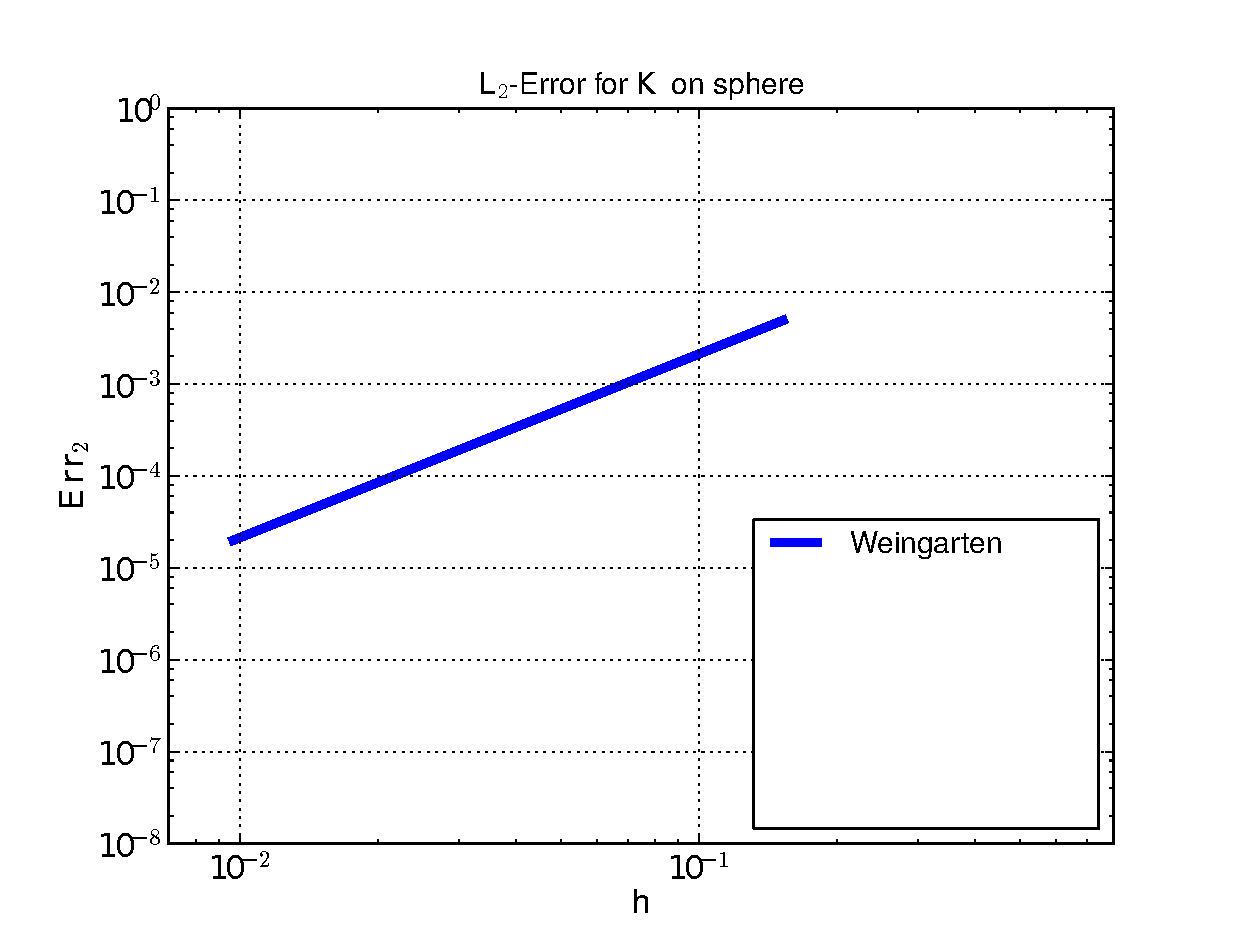
\includegraphics[width=\textwidth]{bilder/Curvature/sphere/ErrKL2_1.eps}
          \end{minipage}\hfill
          \begin{minipage}[t]{0.49\textwidth}
            \centering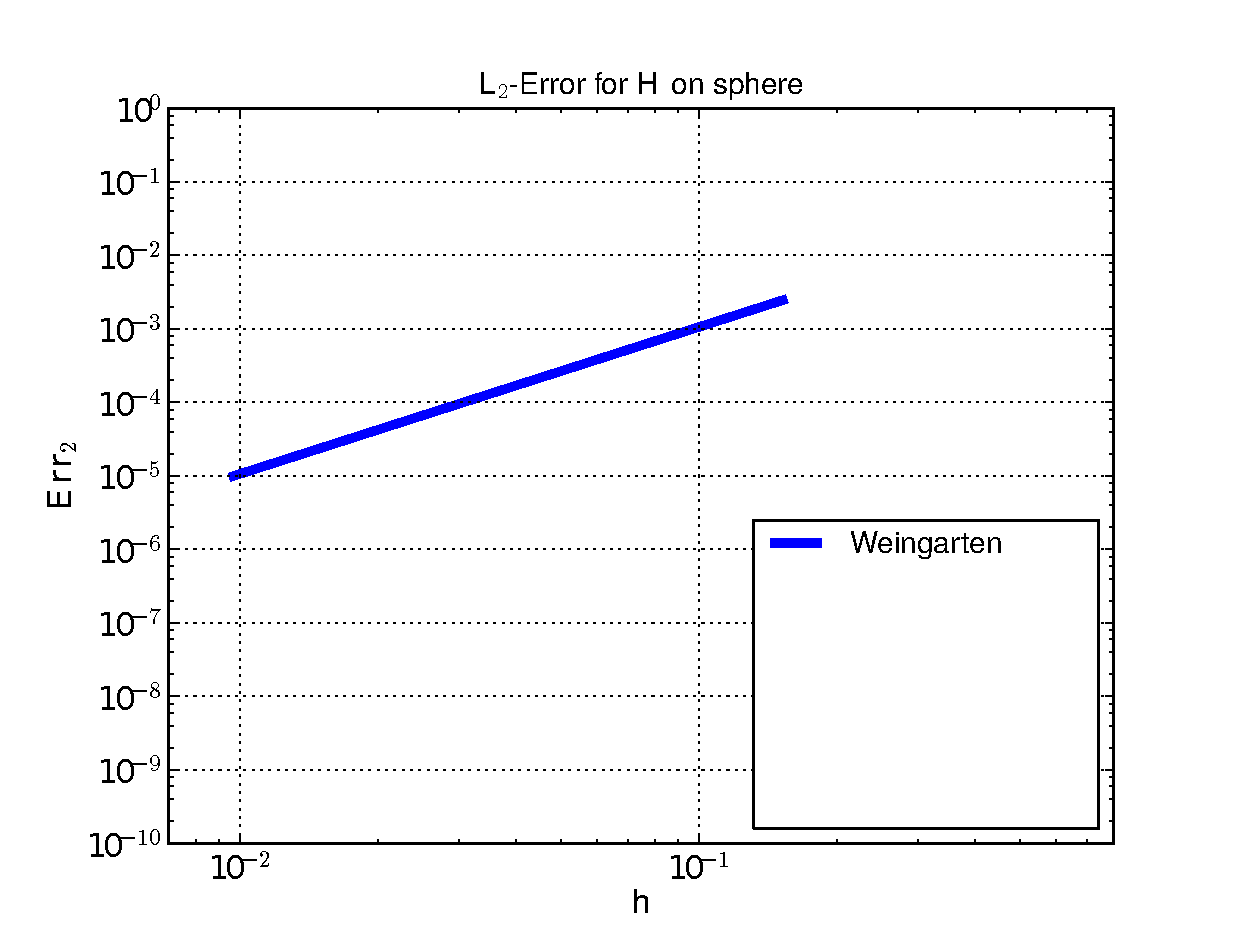
\includegraphics[width=\textwidth]{bilder/Curvature/sphere/ErrHL2_1.eps}
          \end{minipage}
      \onslide<2> 
          \begin{minipage}[t]{0.49\textwidth}
            \centering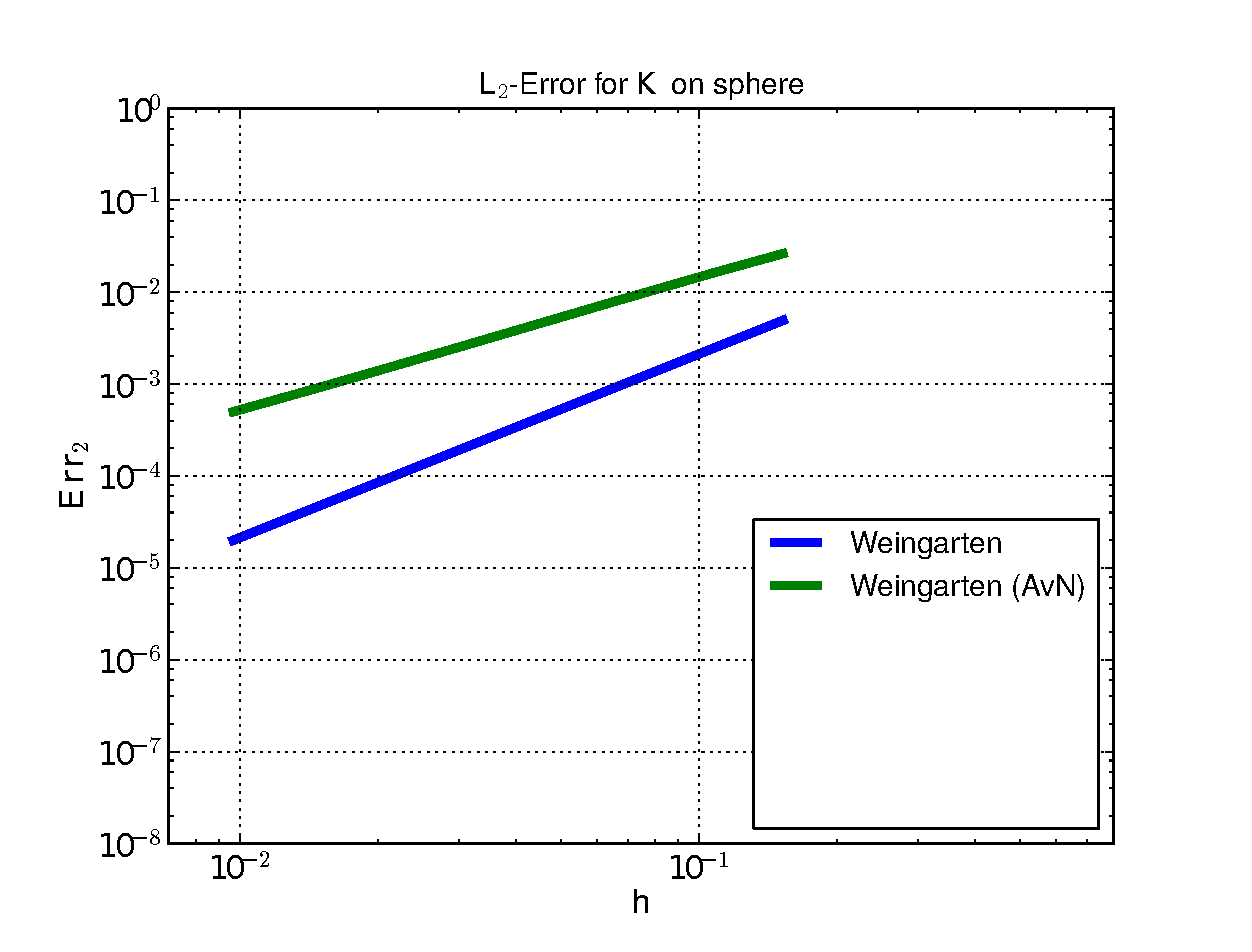
\includegraphics[width=\textwidth]{bilder/Curvature/sphere/ErrKL2_2.eps}
          \end{minipage}\hfill
          \begin{minipage}[t]{0.49\textwidth}
            \centering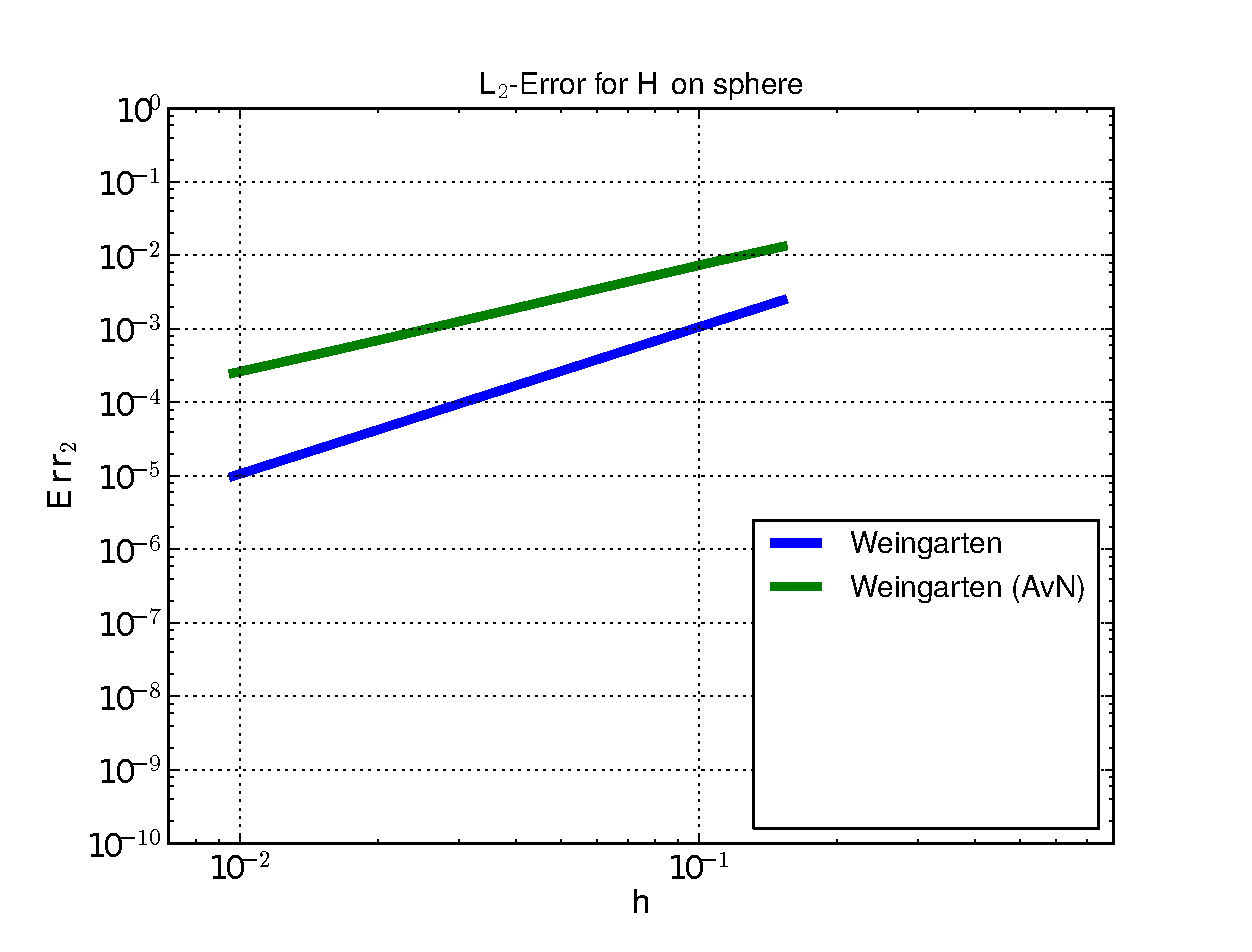
\includegraphics[width=\textwidth]{bilder/Curvature/sphere/ErrHL2_2.eps}
          \end{minipage}
      \onslide<3> 
          \begin{minipage}[t]{0.49\textwidth}
            \centering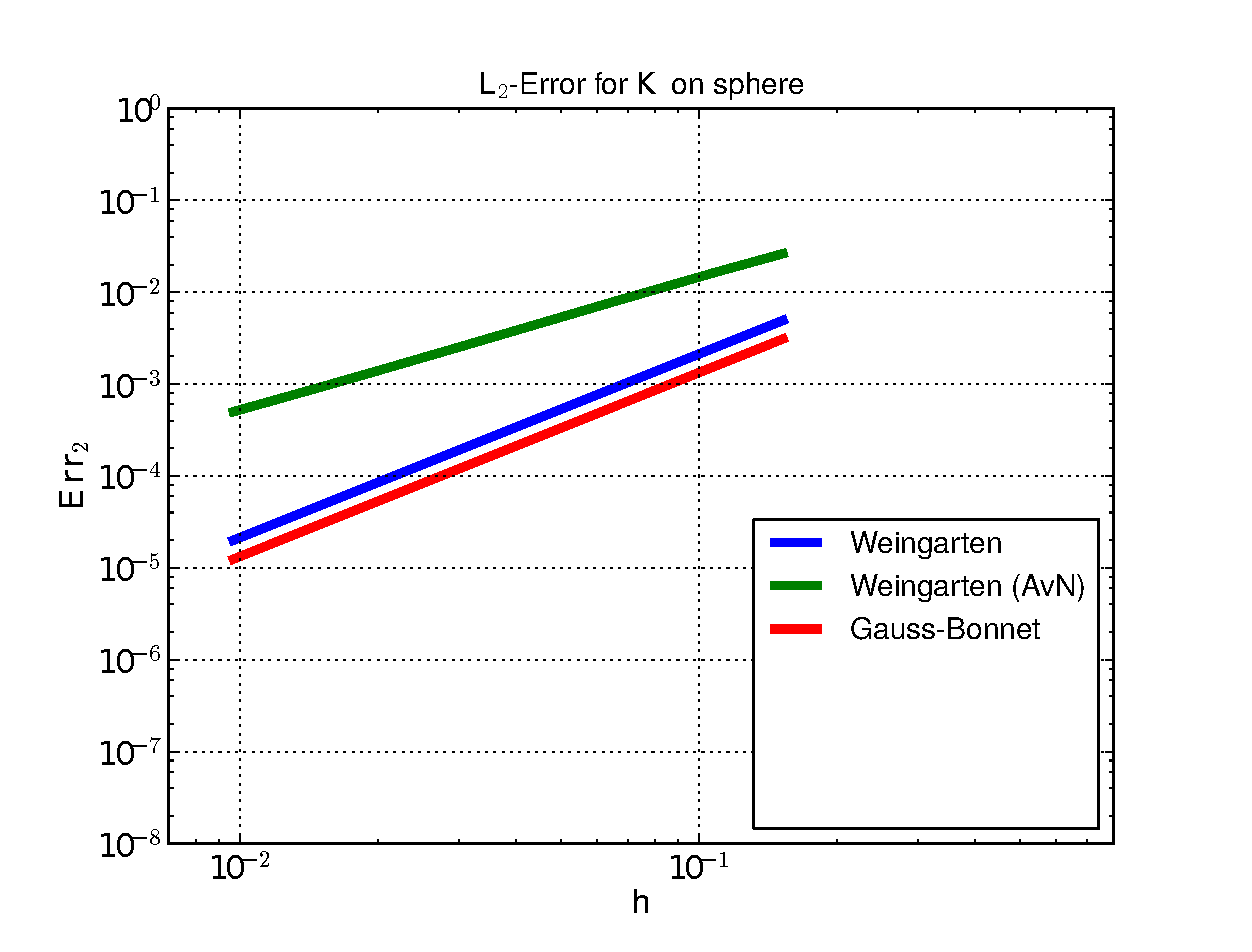
\includegraphics[width=\textwidth]{bilder/Curvature/sphere/ErrKL2_3.eps}
          \end{minipage}\hfill
          \begin{minipage}[t]{0.49\textwidth}
            \centering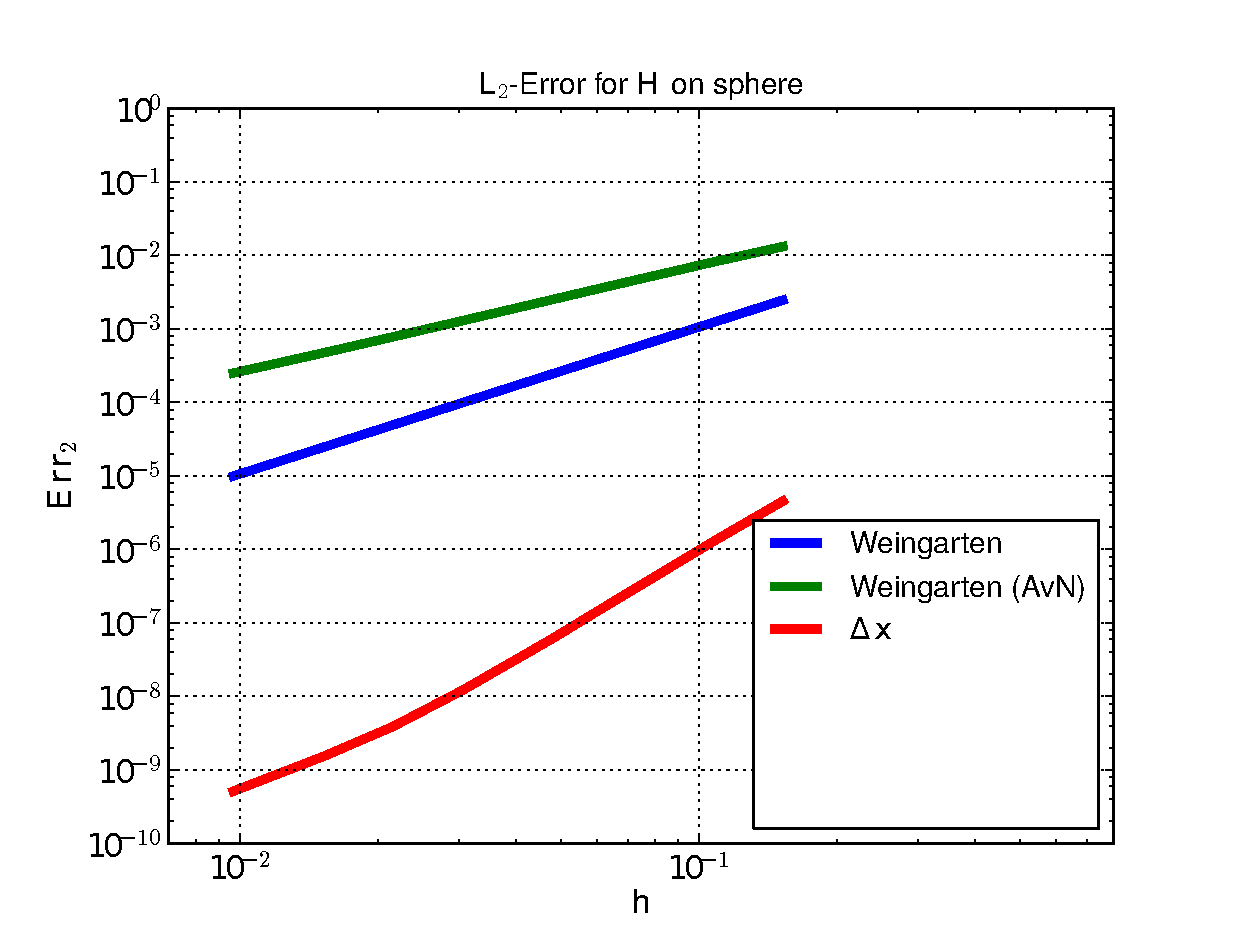
\includegraphics[width=\textwidth]{bilder/Curvature/sphere/ErrHL2_3.eps}
          \end{minipage}
      \onslide<4> 
          \begin{minipage}[t]{0.49\textwidth}
            \centering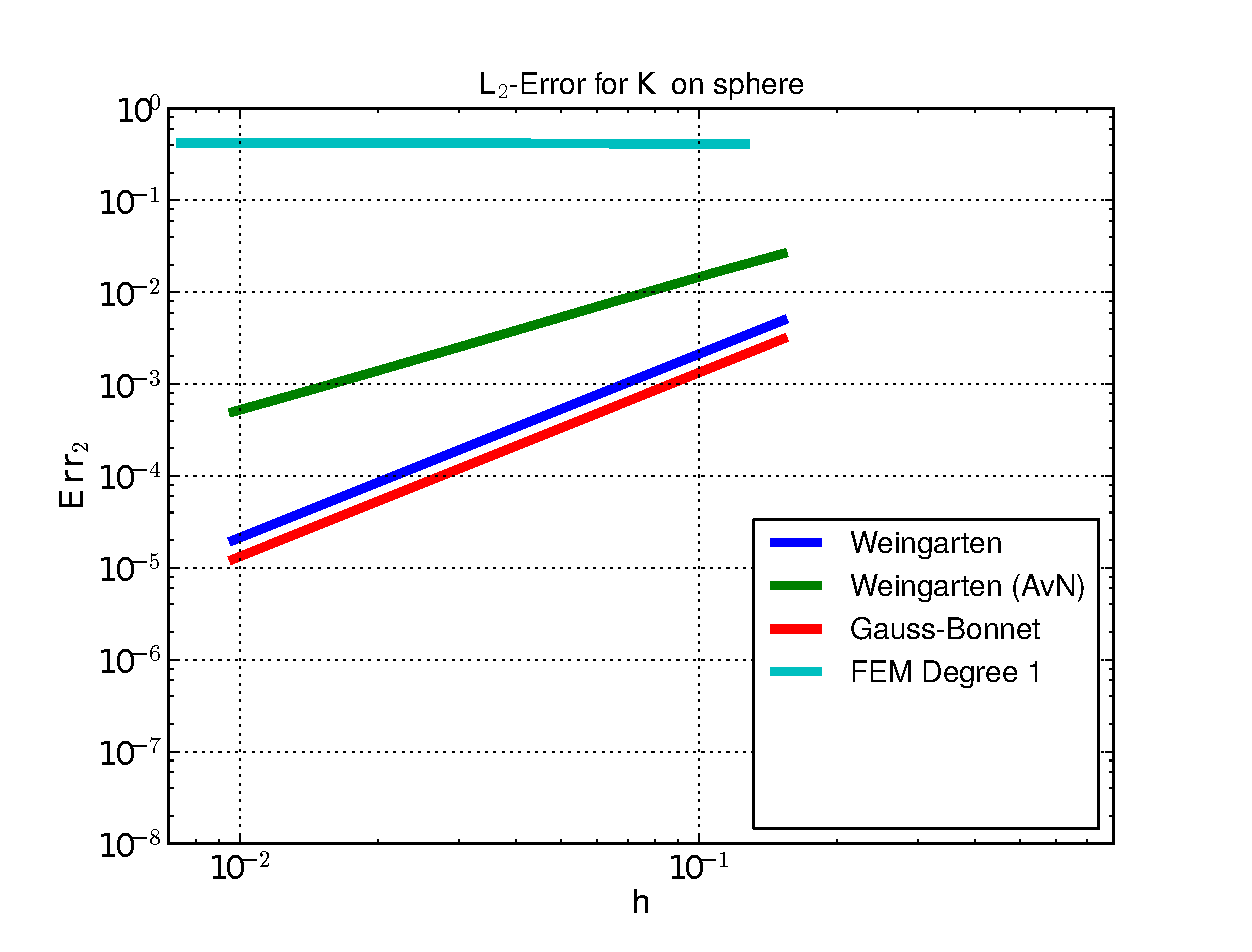
\includegraphics[width=\textwidth]{bilder/Curvature/sphere/ErrKL2_4.eps}
          \end{minipage}\hfill
          \begin{minipage}[t]{0.49\textwidth}
            \centering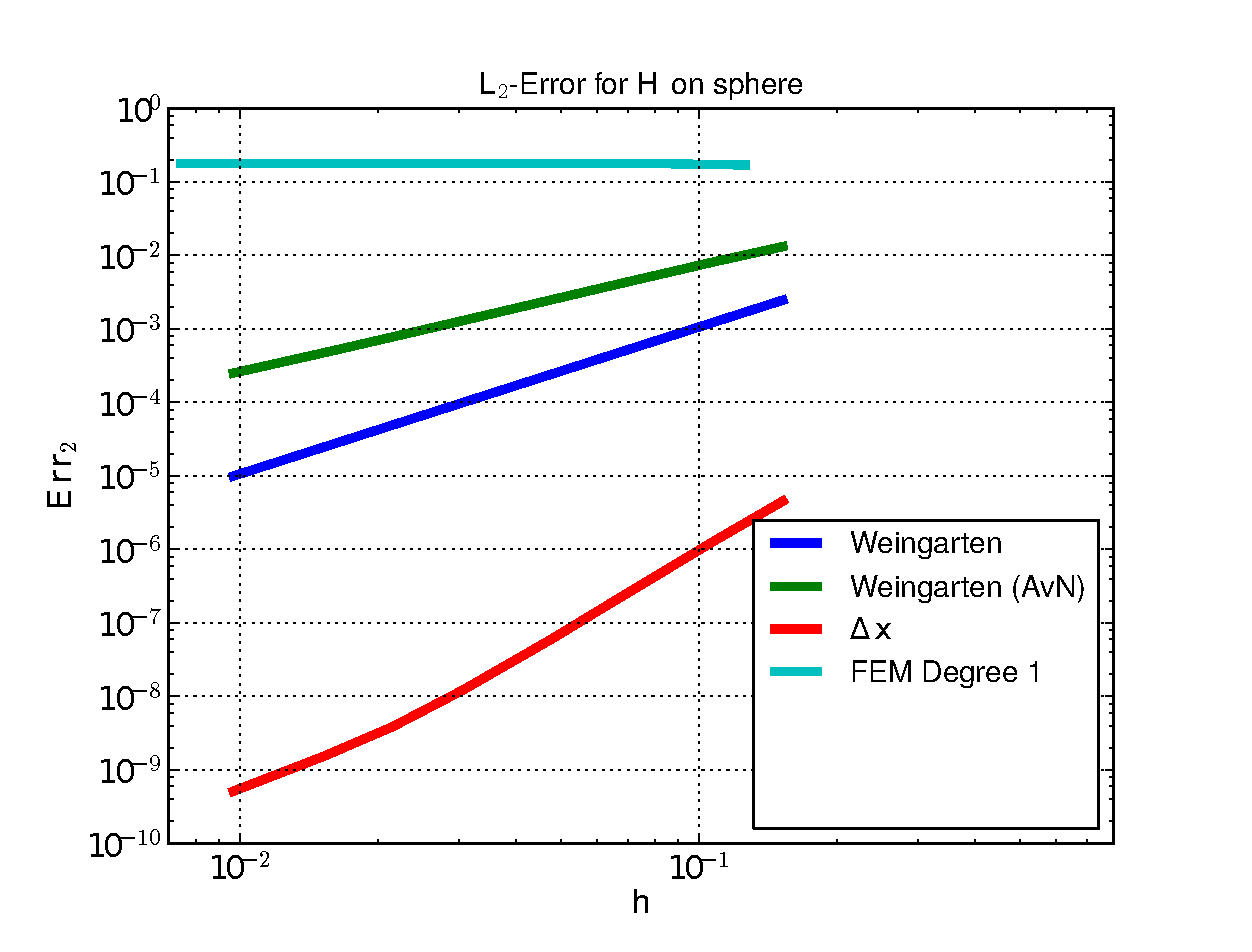
\includegraphics[width=\textwidth]{bilder/Curvature/sphere/ErrHL2_4.eps}
          \end{minipage}
      \onslide<5> 
          \begin{minipage}[t]{0.49\textwidth}
            \centering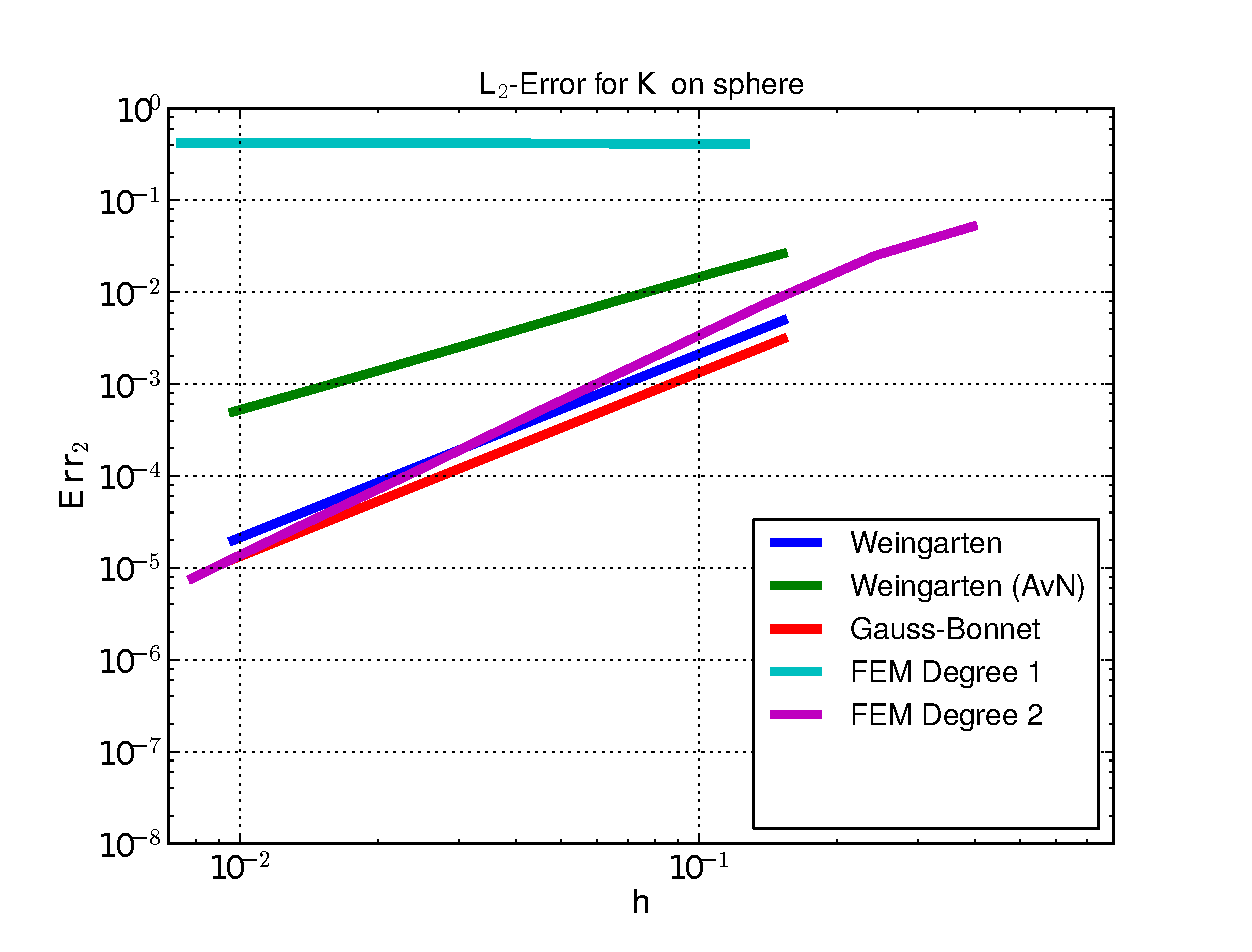
\includegraphics[width=\textwidth]{bilder/Curvature/sphere/ErrKL2_5.eps}
          \end{minipage}\hfill
          \begin{minipage}[t]{0.49\textwidth}
            \centering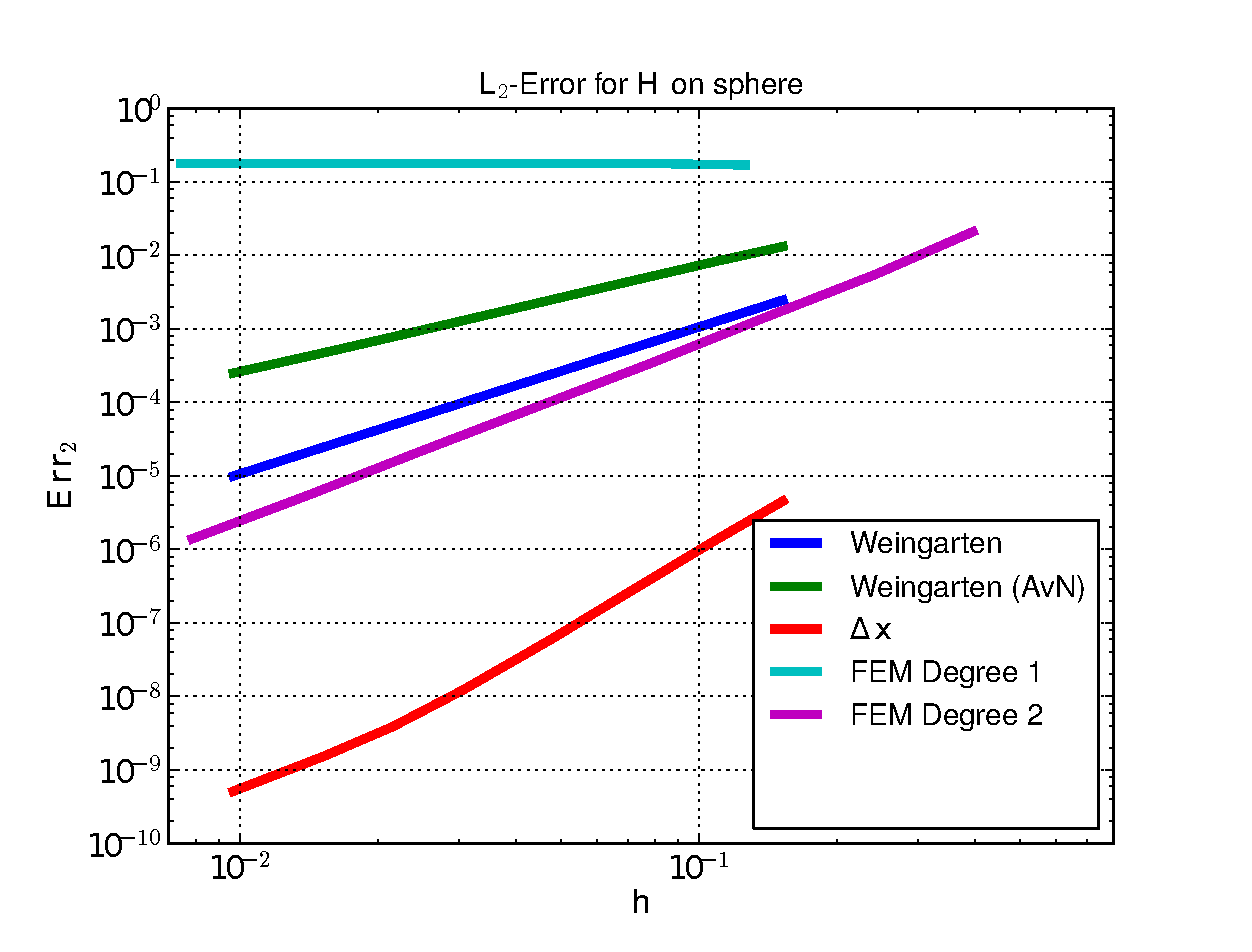
\includegraphics[width=\textwidth]{bilder/Curvature/sphere/ErrHL2_5.eps}
          \end{minipage}
      \onslide<6> 
          \begin{minipage}[t]{0.49\textwidth}
            \centering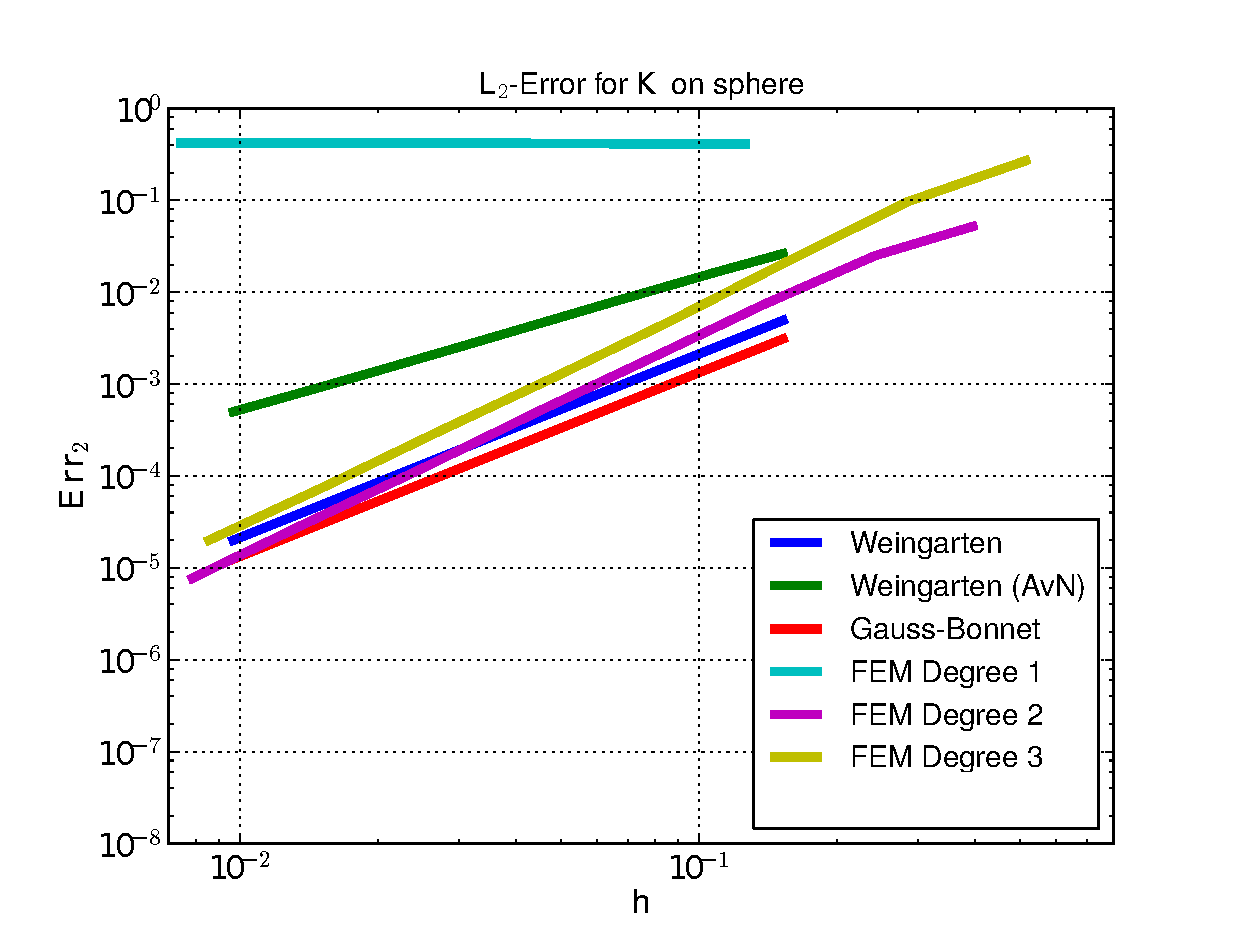
\includegraphics[width=\textwidth]{bilder/Curvature/sphere/ErrKL2_6.eps}
          \end{minipage}\hfill
          \begin{minipage}[t]{0.49\textwidth}
            \centering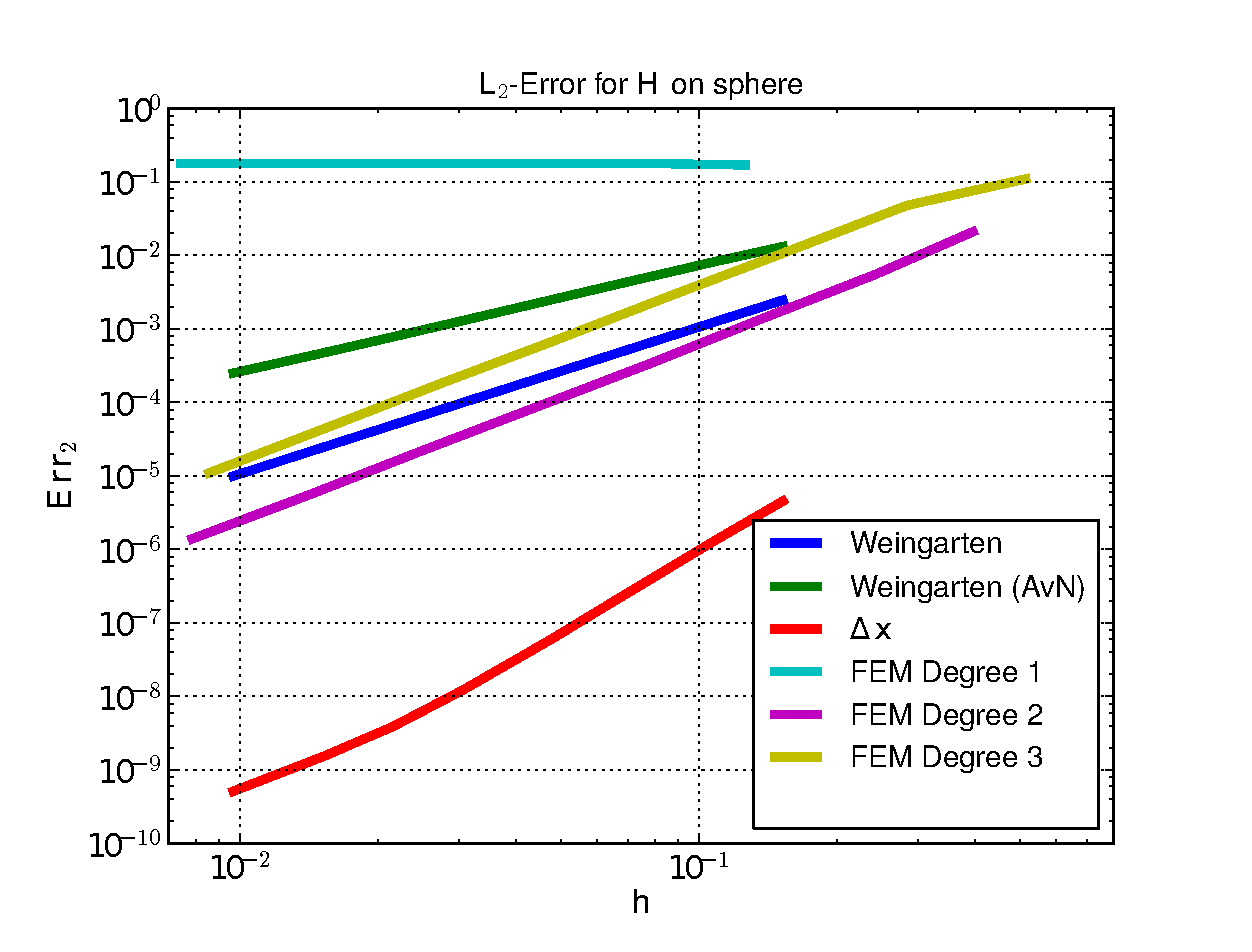
\includegraphics[width=\textwidth]{bilder/Curvature/sphere/ErrHL2_6.eps}
          \end{minipage}
      \onslide<7> 
          \begin{minipage}[t]{0.49\textwidth}
            \centering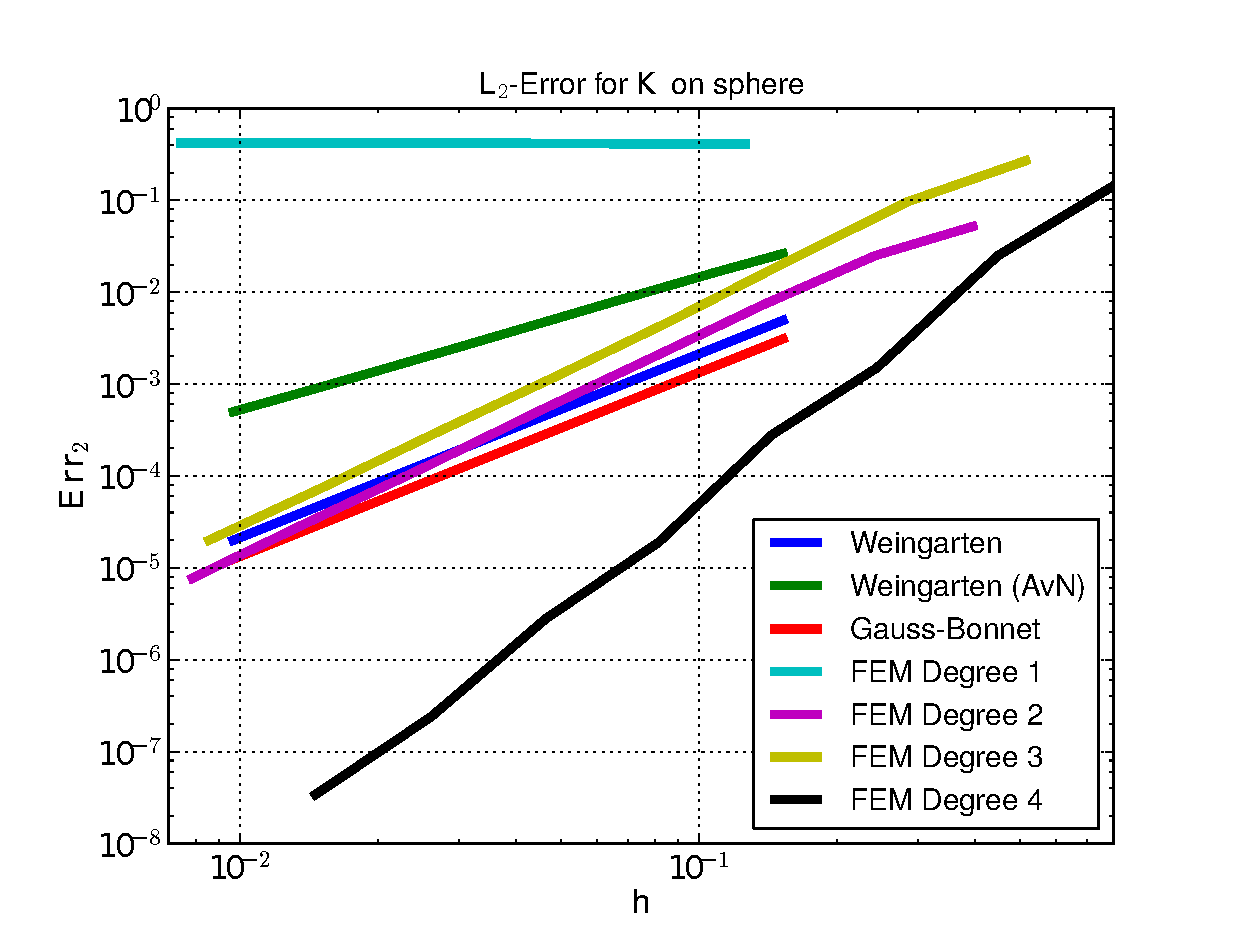
\includegraphics[width=\textwidth]{bilder/Curvature/sphere/ErrKL2_7.eps}
          \end{minipage}\hfill
          \begin{minipage}[t]{0.49\textwidth}
            \centering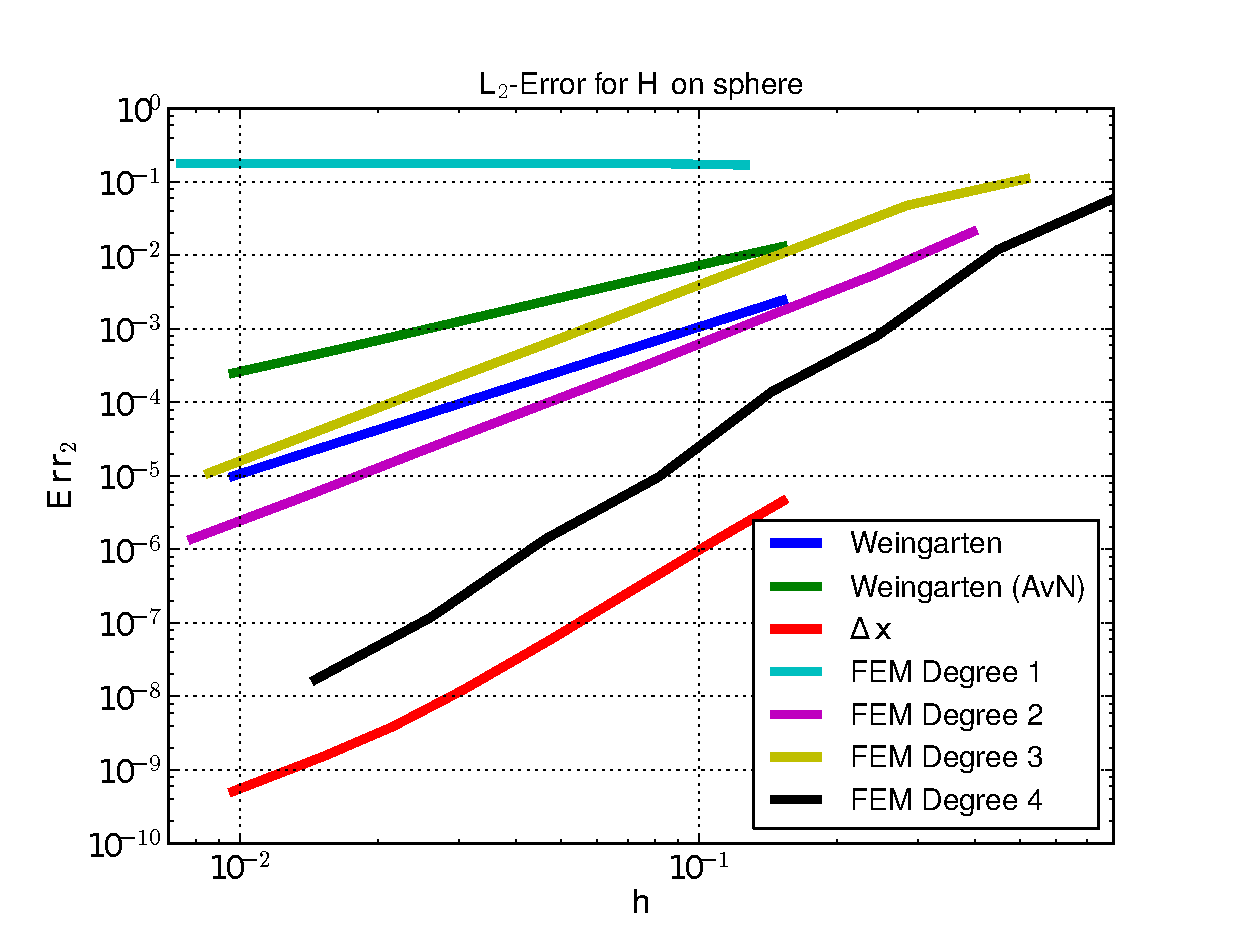
\includegraphics[width=\textwidth]{bilder/Curvature/sphere/ErrHL2_7.eps}
          \end{minipage}
      %elipsoid
      \onslide<8>
           \begin{minipage}[t]{0.49\textwidth}
              \centering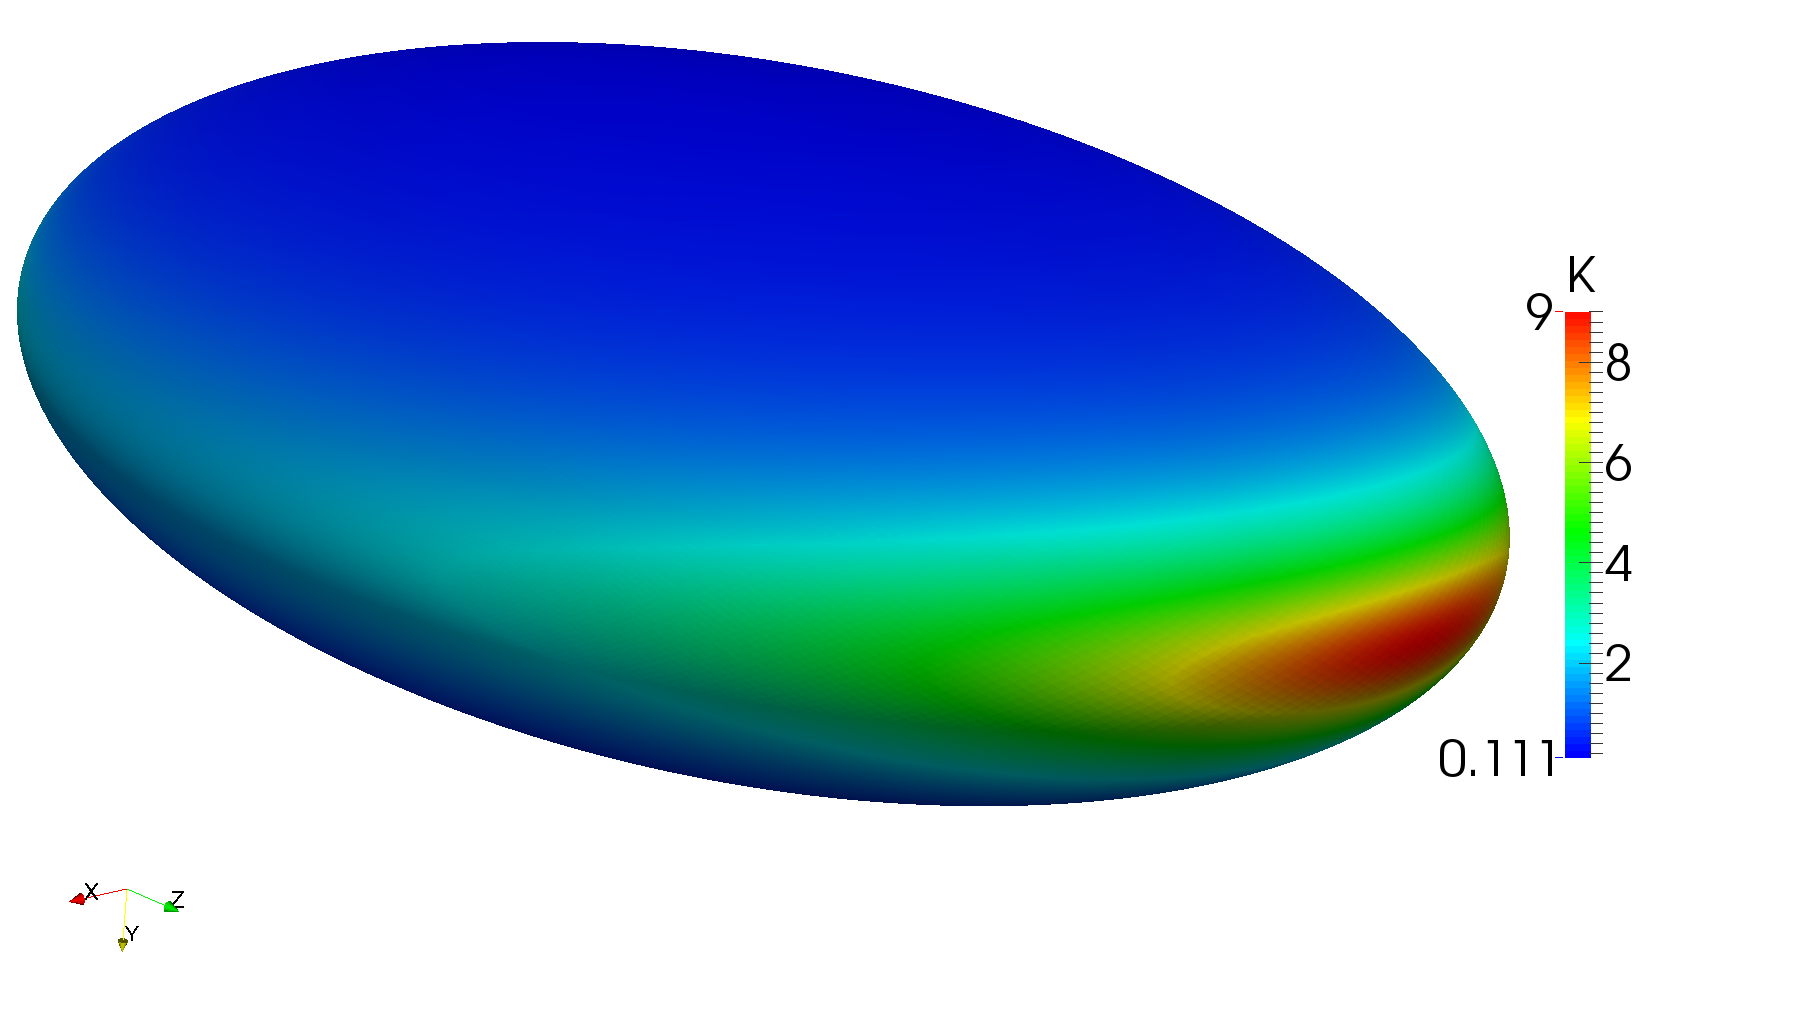
\includegraphics[width=\textwidth]{bilder/Curvature/heineC/K2k.png}
            \end{minipage}\hfill
            \begin{minipage}[t]{0.49\textwidth}
              \centering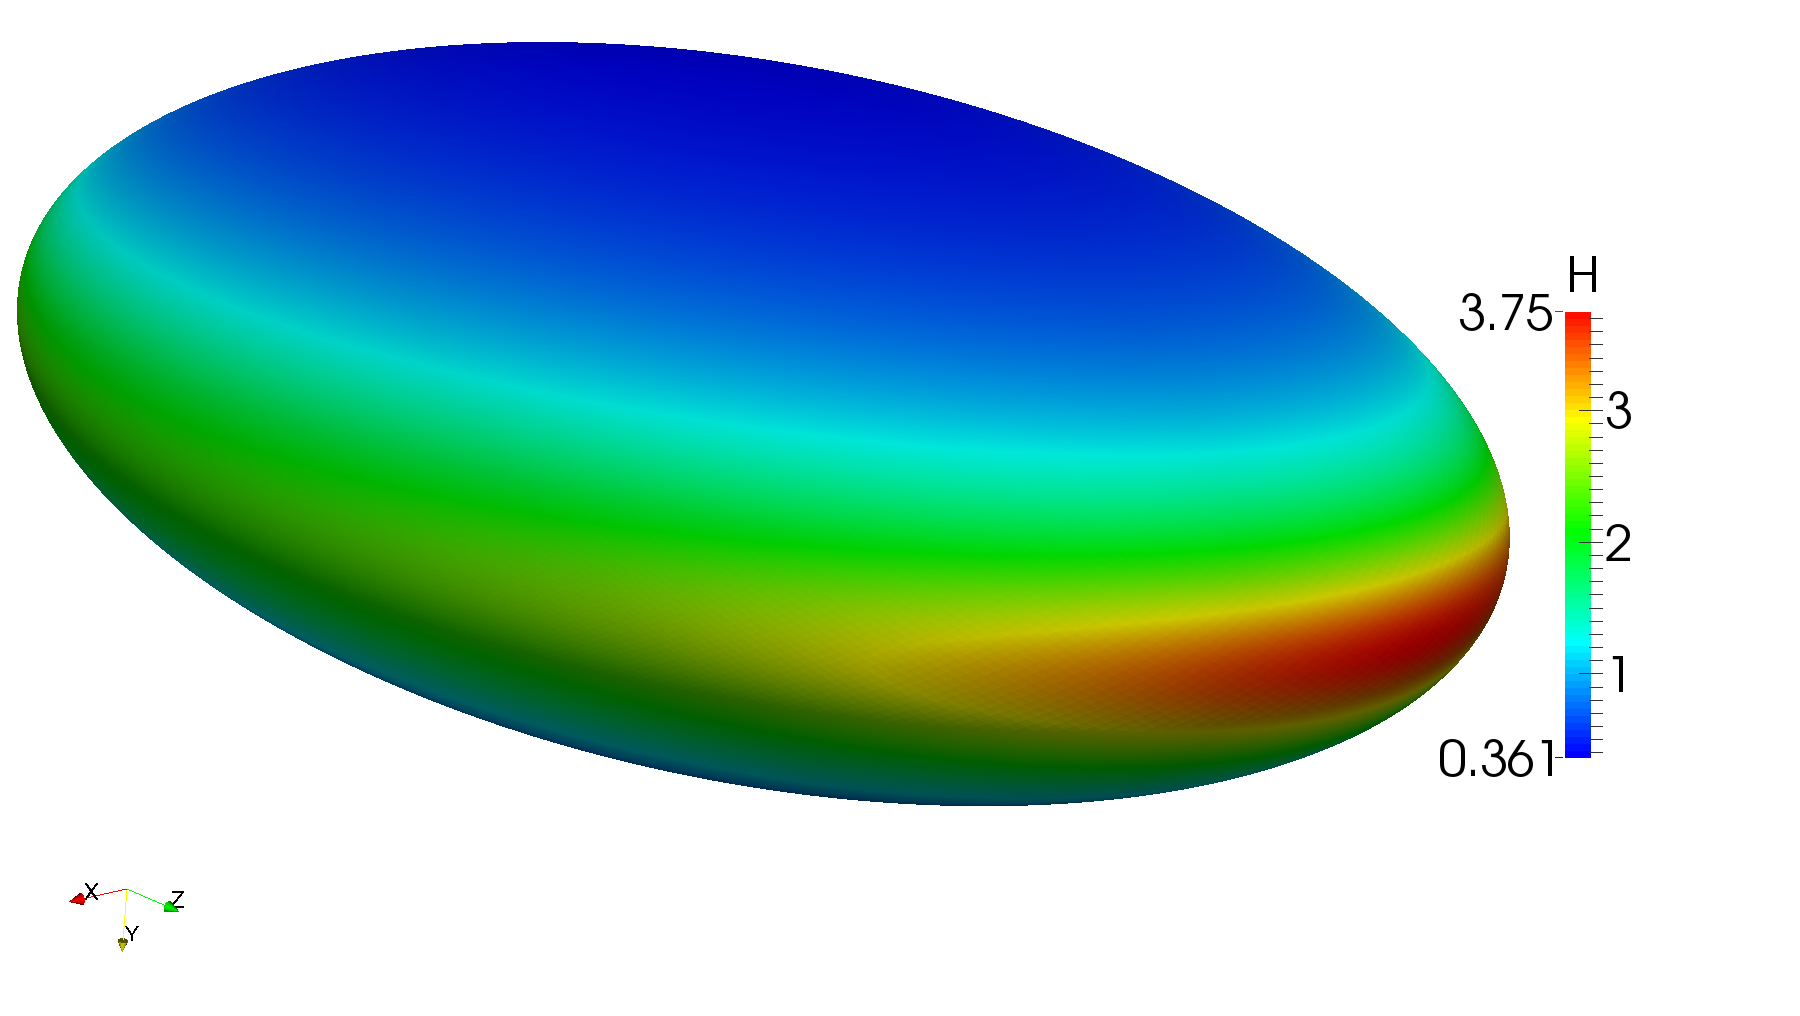
\includegraphics[width=\textwidth]{bilder/Curvature/heineC/H2k.png}
            \end{minipage}
      \onslide<9> 
          \begin{minipage}[t]{0.49\textwidth}
            \centering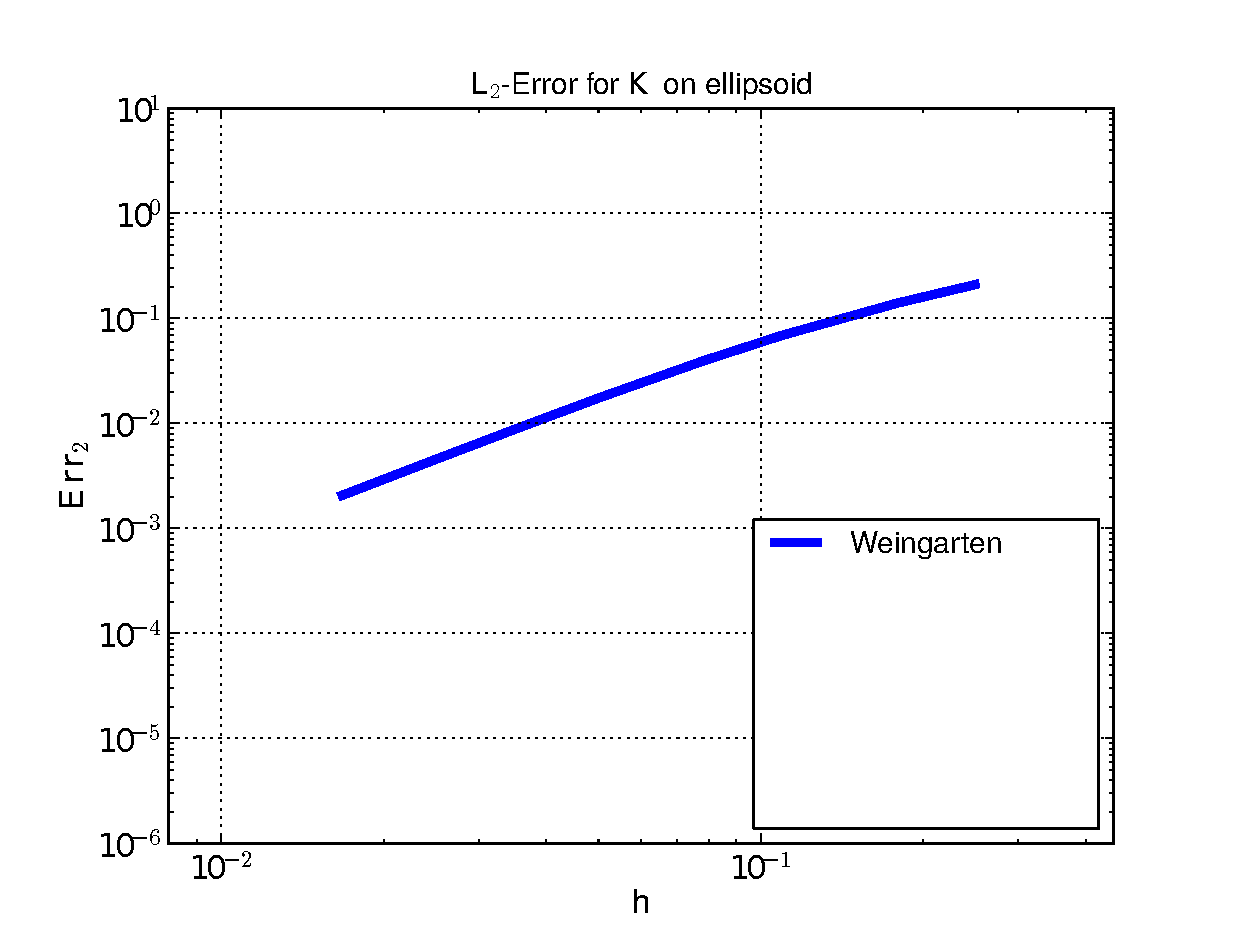
\includegraphics[width=\textwidth]{bilder/Curvature/heineC/ErrKL2_1.eps}
          \end{minipage}\hfill
          \begin{minipage}[t]{0.49\textwidth}
            \centering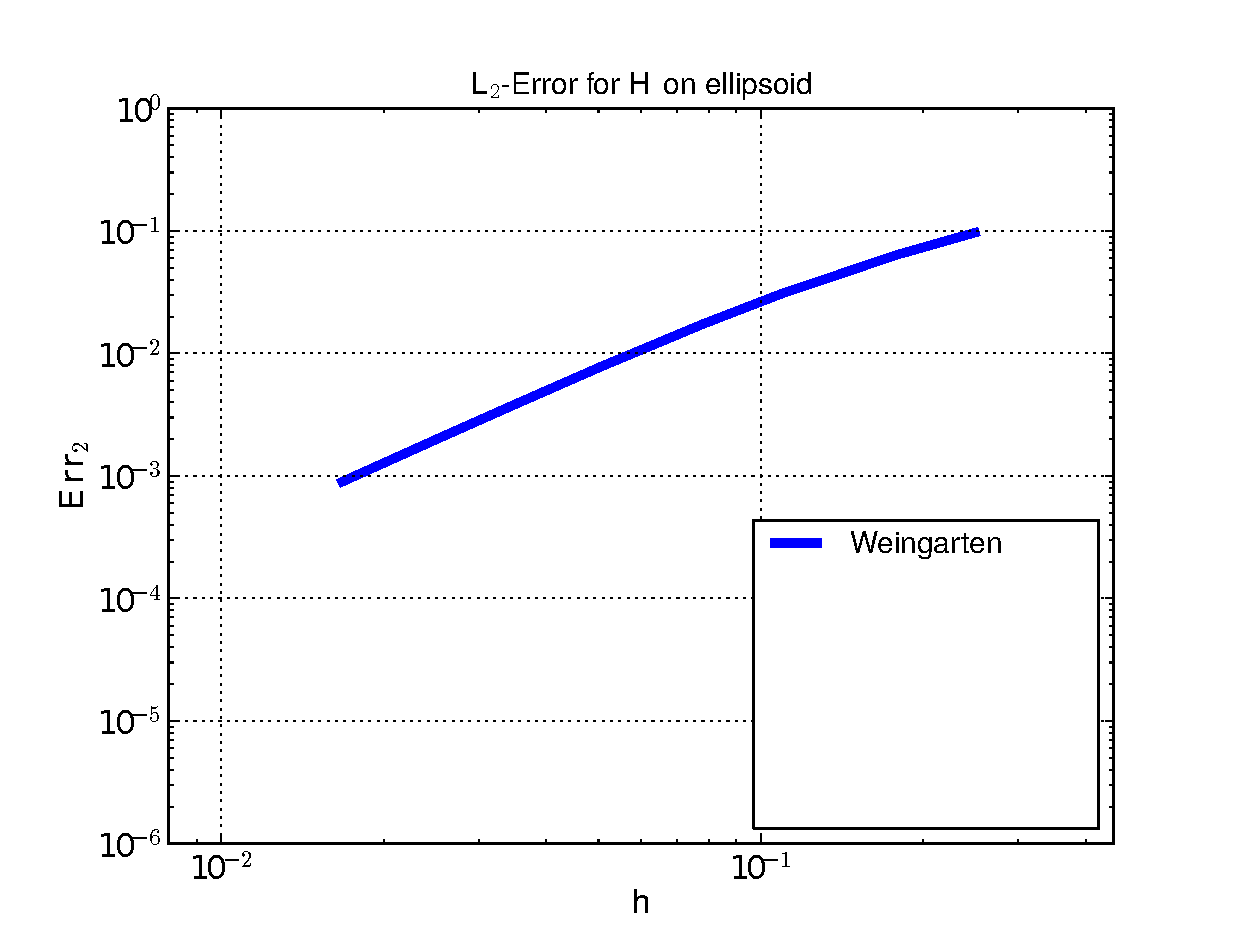
\includegraphics[width=\textwidth]{bilder/Curvature/heineC/ErrHL2_1.eps}
          \end{minipage}
      \onslide<10> 
          \begin{minipage}[t]{0.49\textwidth}
            \centering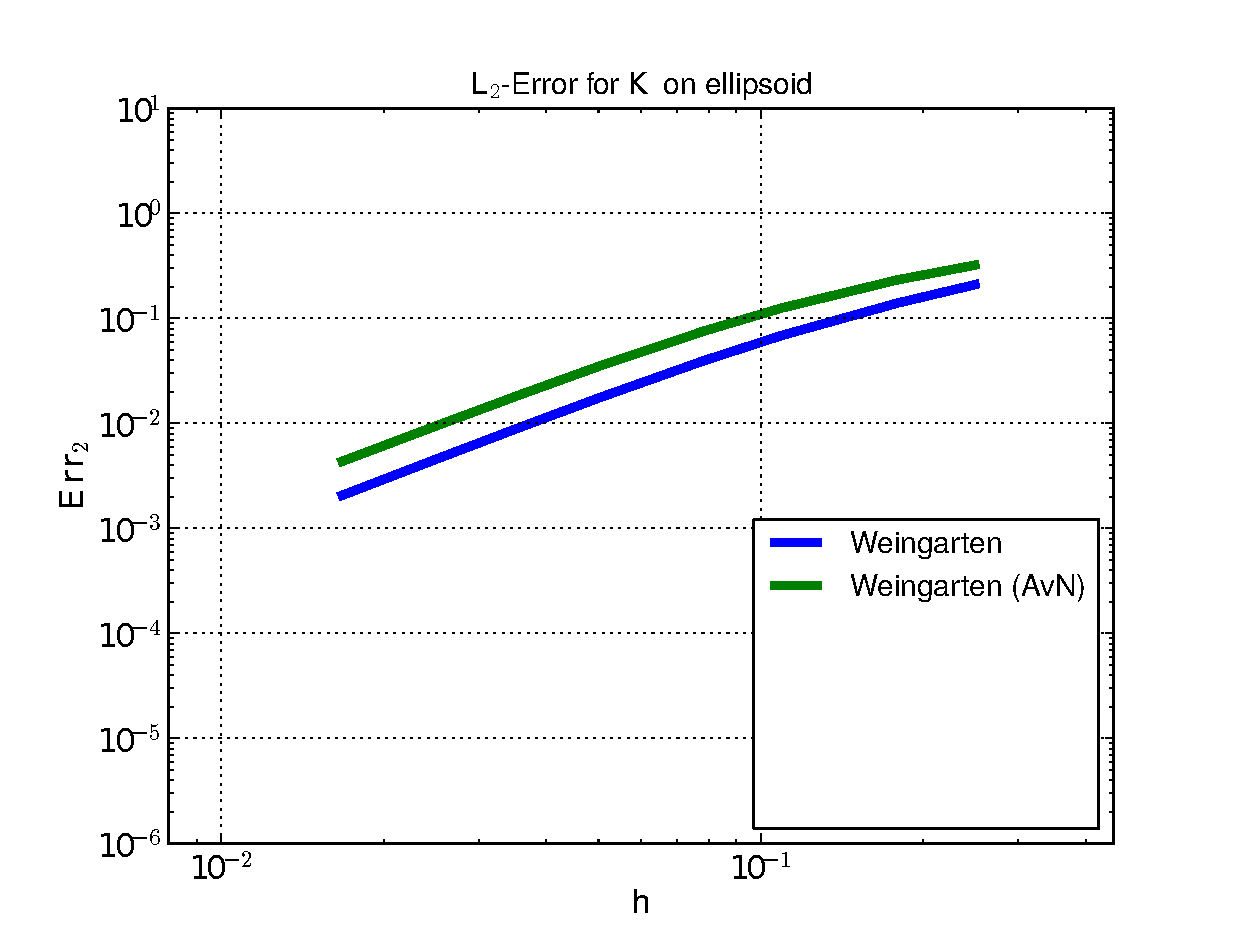
\includegraphics[width=\textwidth]{bilder/Curvature/heineC/ErrKL2_2.eps}
          \end{minipage}\hfill
          \begin{minipage}[t]{0.49\textwidth}
            \centering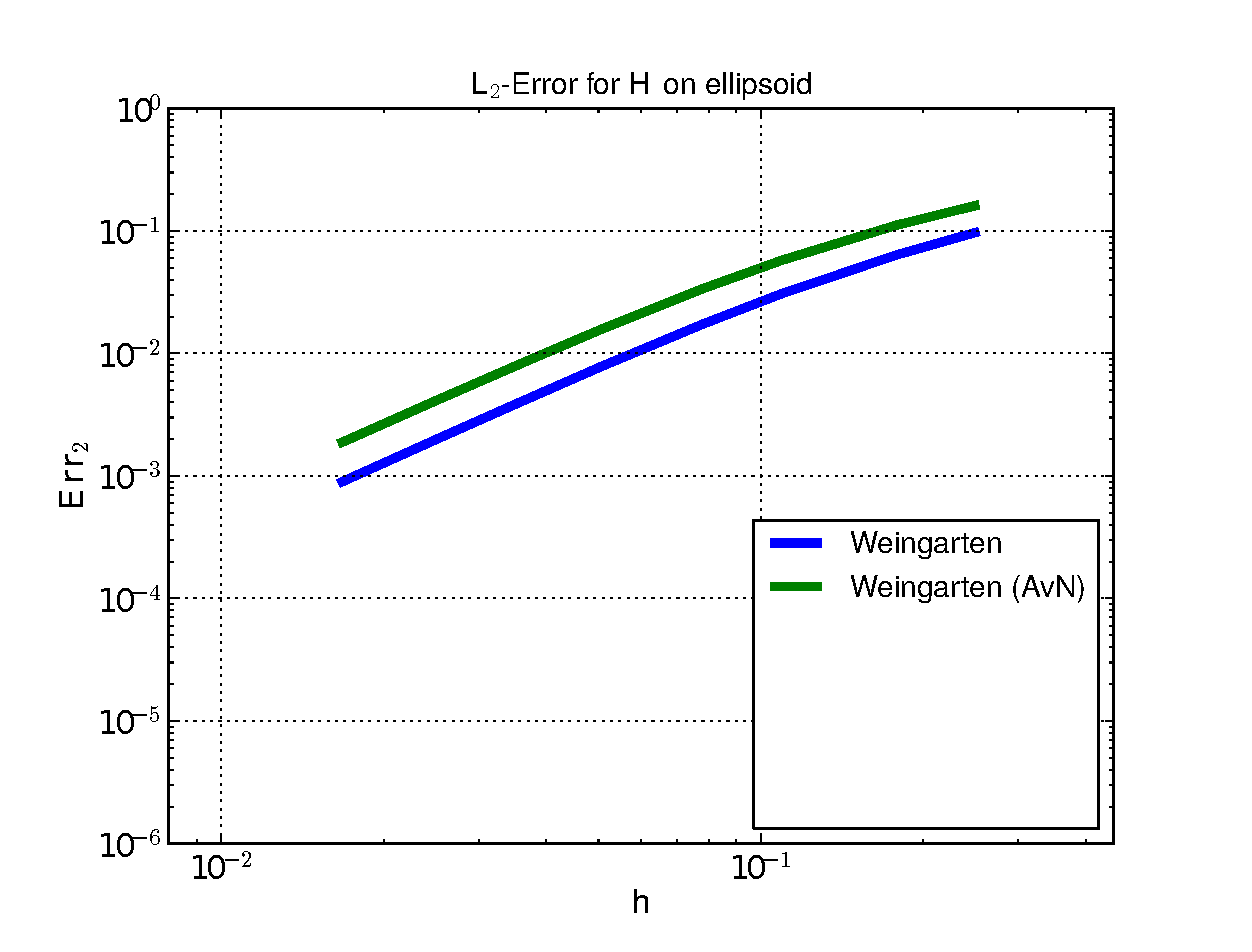
\includegraphics[width=\textwidth]{bilder/Curvature/heineC/ErrHL2_2.eps}
          \end{minipage}
      \onslide<11> 
          \begin{minipage}[t]{0.49\textwidth}
            \centering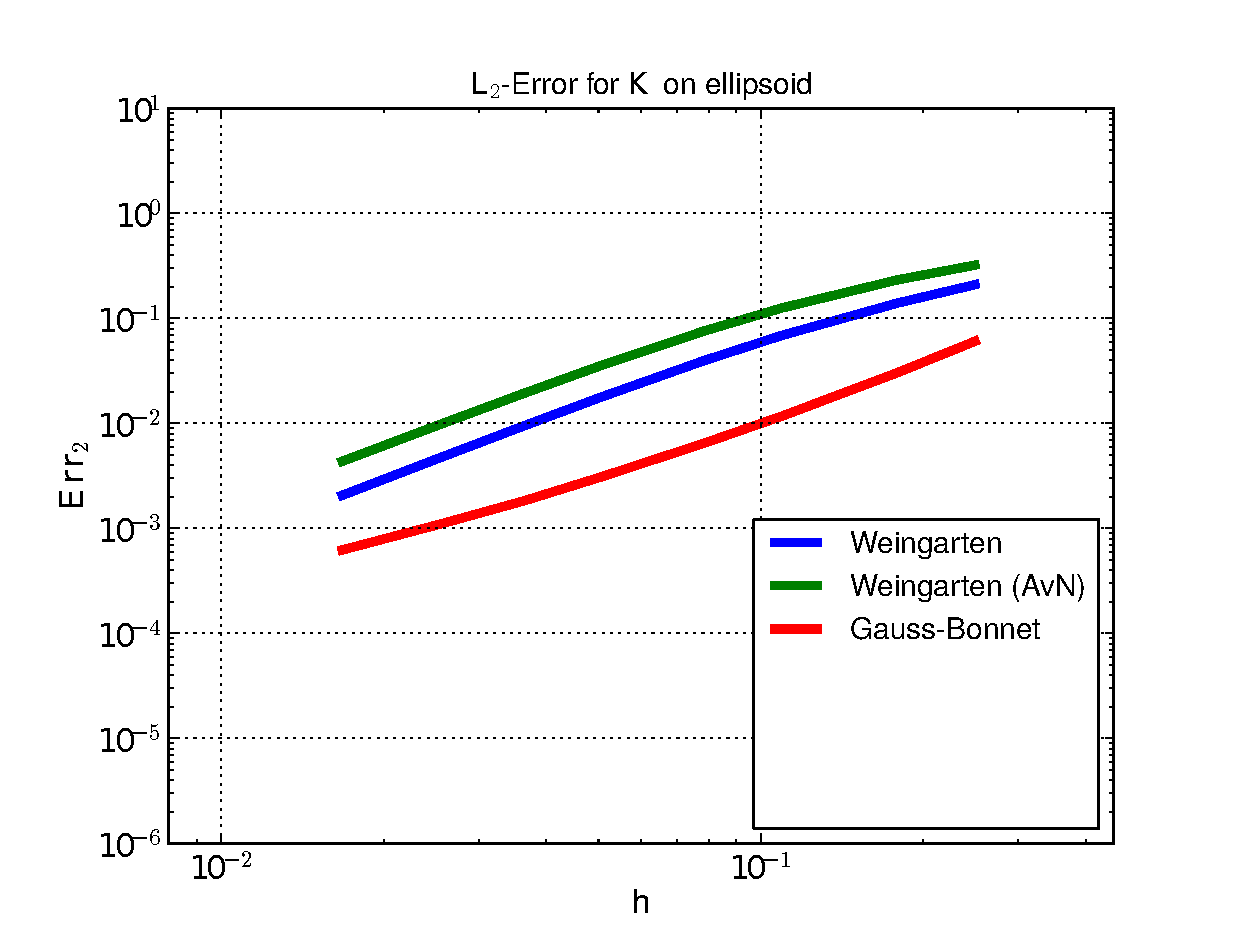
\includegraphics[width=\textwidth]{bilder/Curvature/heineC/ErrKL2_3.eps}
          \end{minipage}\hfill
          \begin{minipage}[t]{0.49\textwidth}
            \centering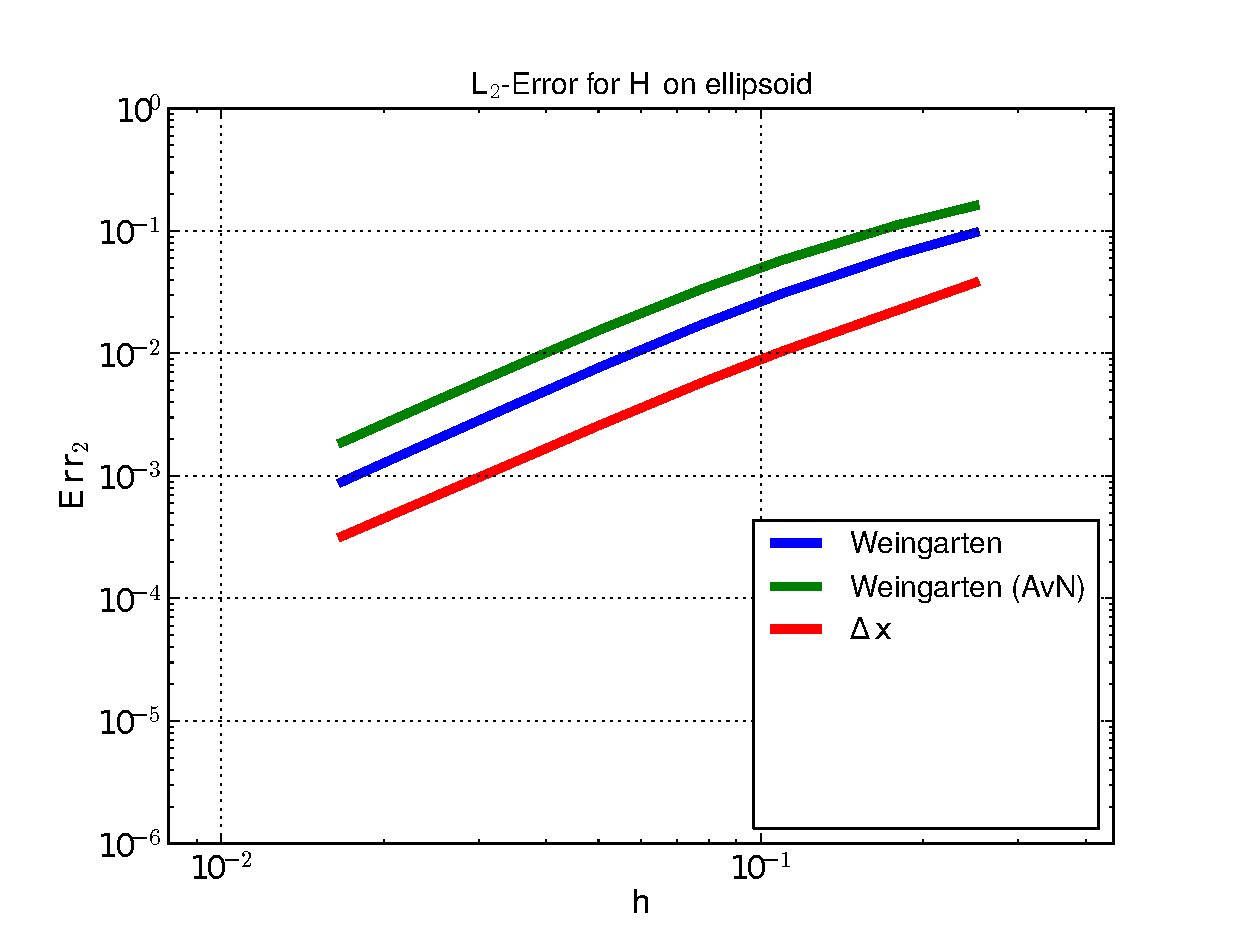
\includegraphics[width=\textwidth]{bilder/Curvature/heineC/ErrHL2_3.eps}
          \end{minipage}
      \onslide<12> 
          \begin{minipage}[t]{0.49\textwidth}
            \centering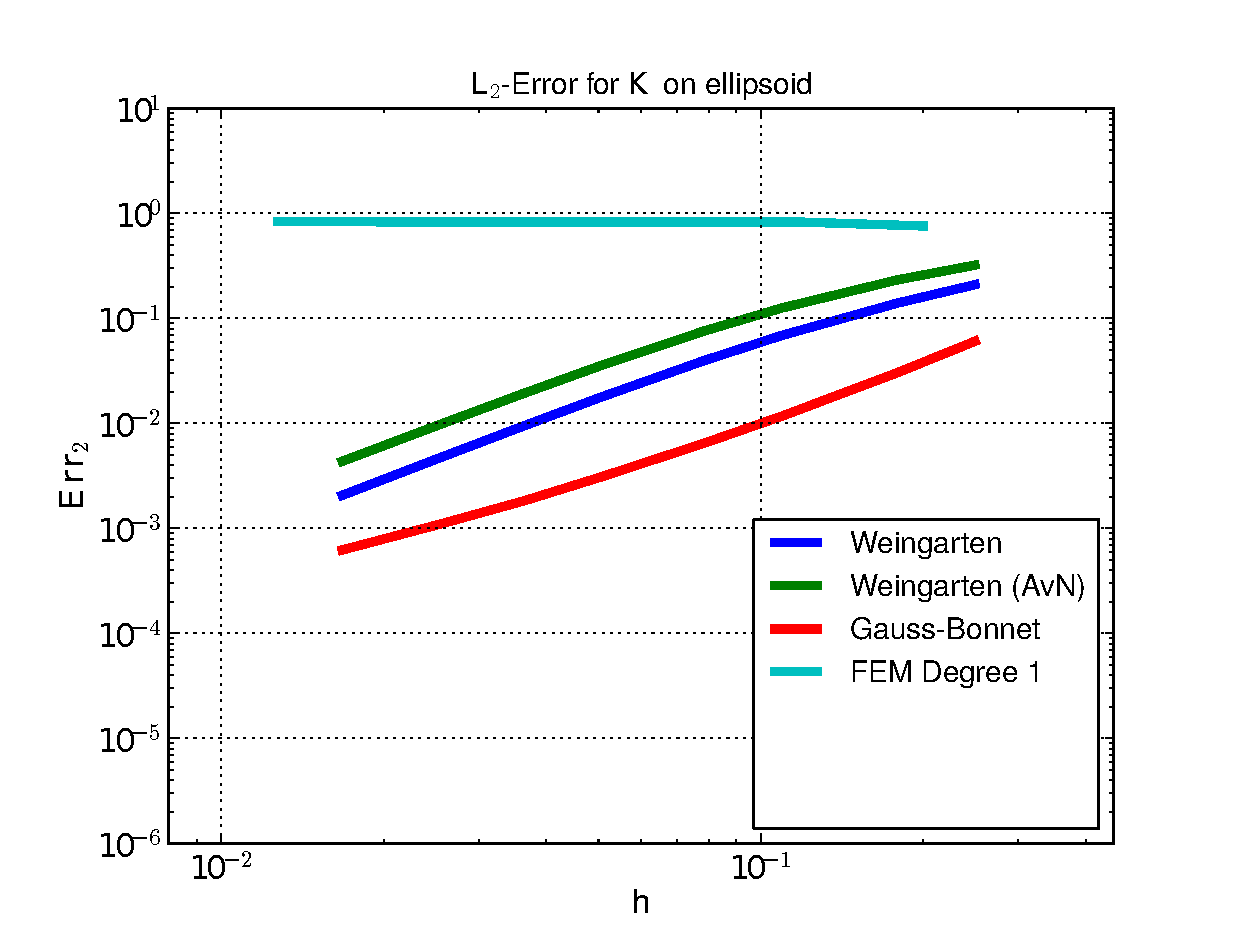
\includegraphics[width=\textwidth]{bilder/Curvature/heineC/ErrKL2_4.eps}
          \end{minipage}\hfill
          \begin{minipage}[t]{0.49\textwidth}
            \centering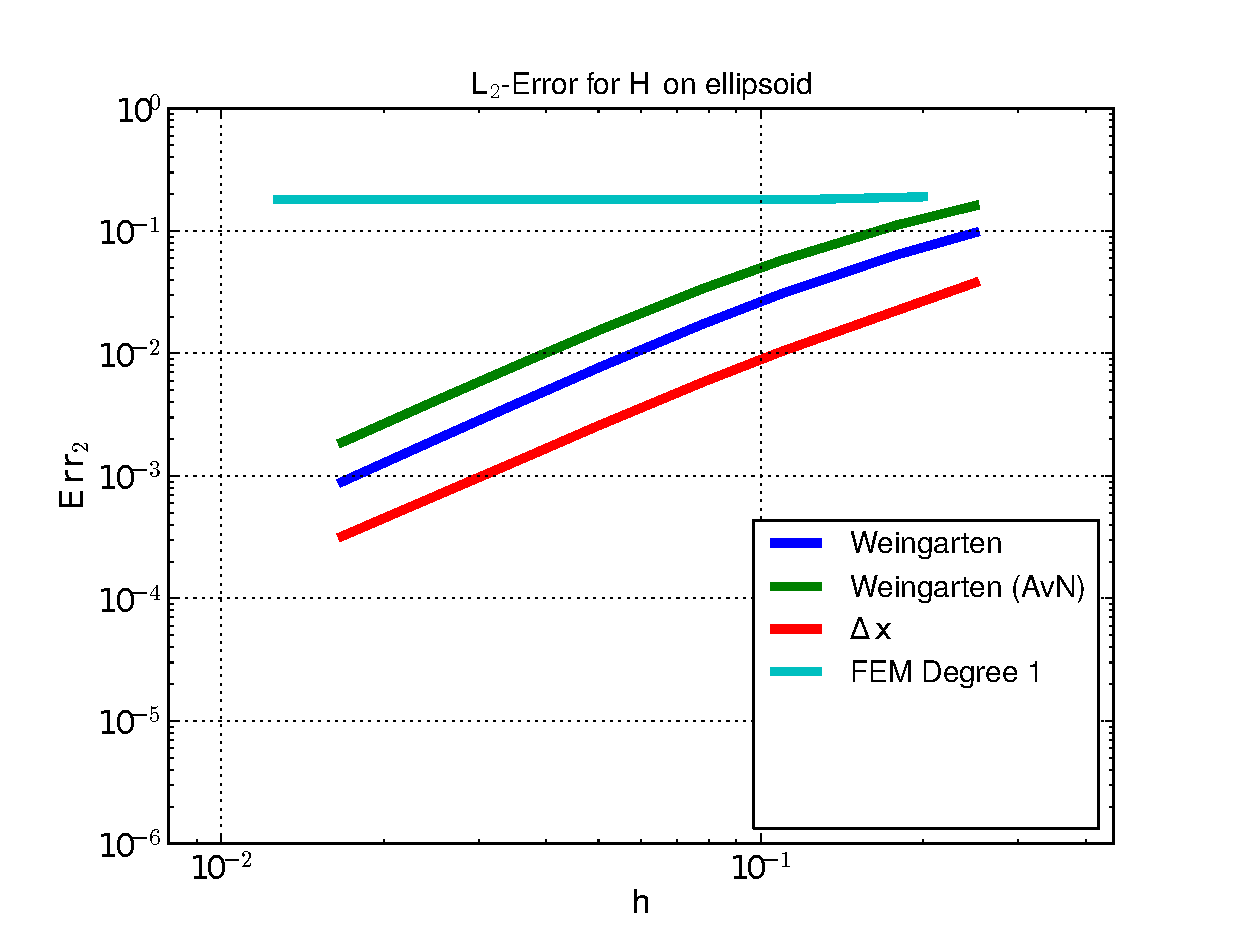
\includegraphics[width=\textwidth]{bilder/Curvature/heineC/ErrHL2_4.eps}
          \end{minipage}
      \onslide<13> 
          \begin{minipage}[t]{0.49\textwidth}
            \centering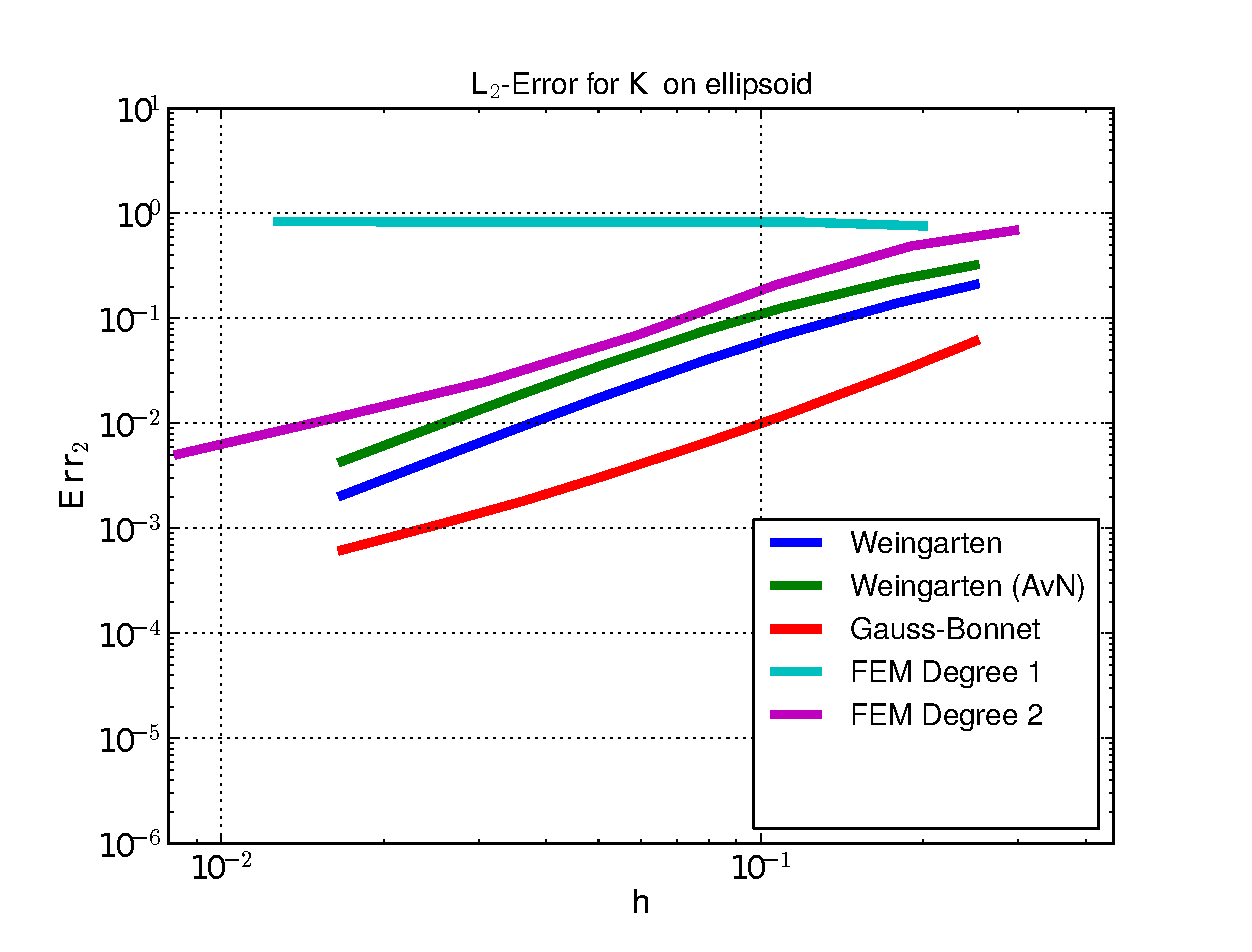
\includegraphics[width=\textwidth]{bilder/Curvature/heineC/ErrKL2_5.eps}
          \end{minipage}\hfill
          \begin{minipage}[t]{0.49\textwidth}
            \centering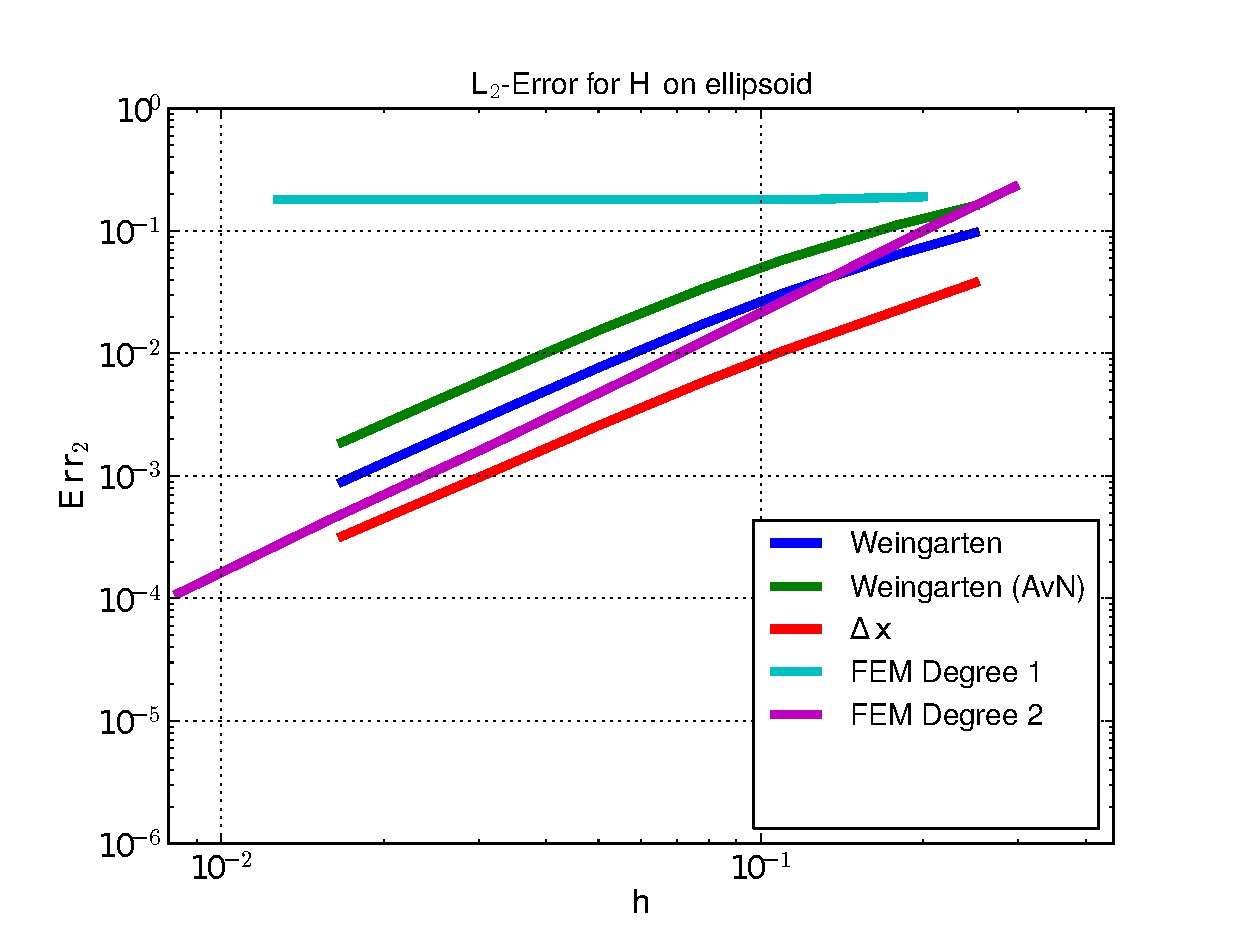
\includegraphics[width=\textwidth]{bilder/Curvature/heineC/ErrHL2_5.eps}
          \end{minipage}
      \onslide<14> 
          \begin{minipage}[t]{0.49\textwidth}
            \centering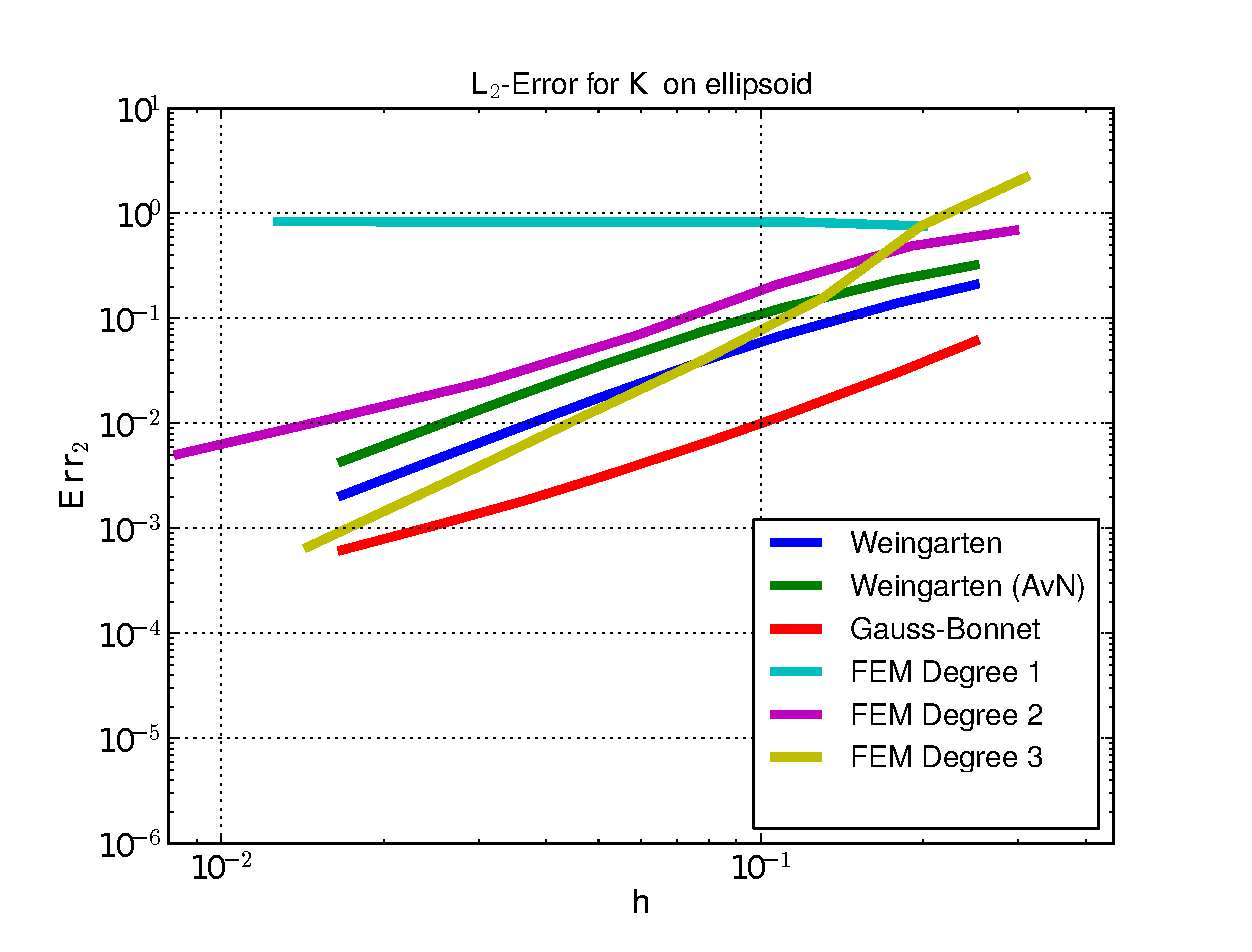
\includegraphics[width=\textwidth]{bilder/Curvature/heineC/ErrKL2_6.eps}
          \end{minipage}\hfill
          \begin{minipage}[t]{0.49\textwidth}
            \centering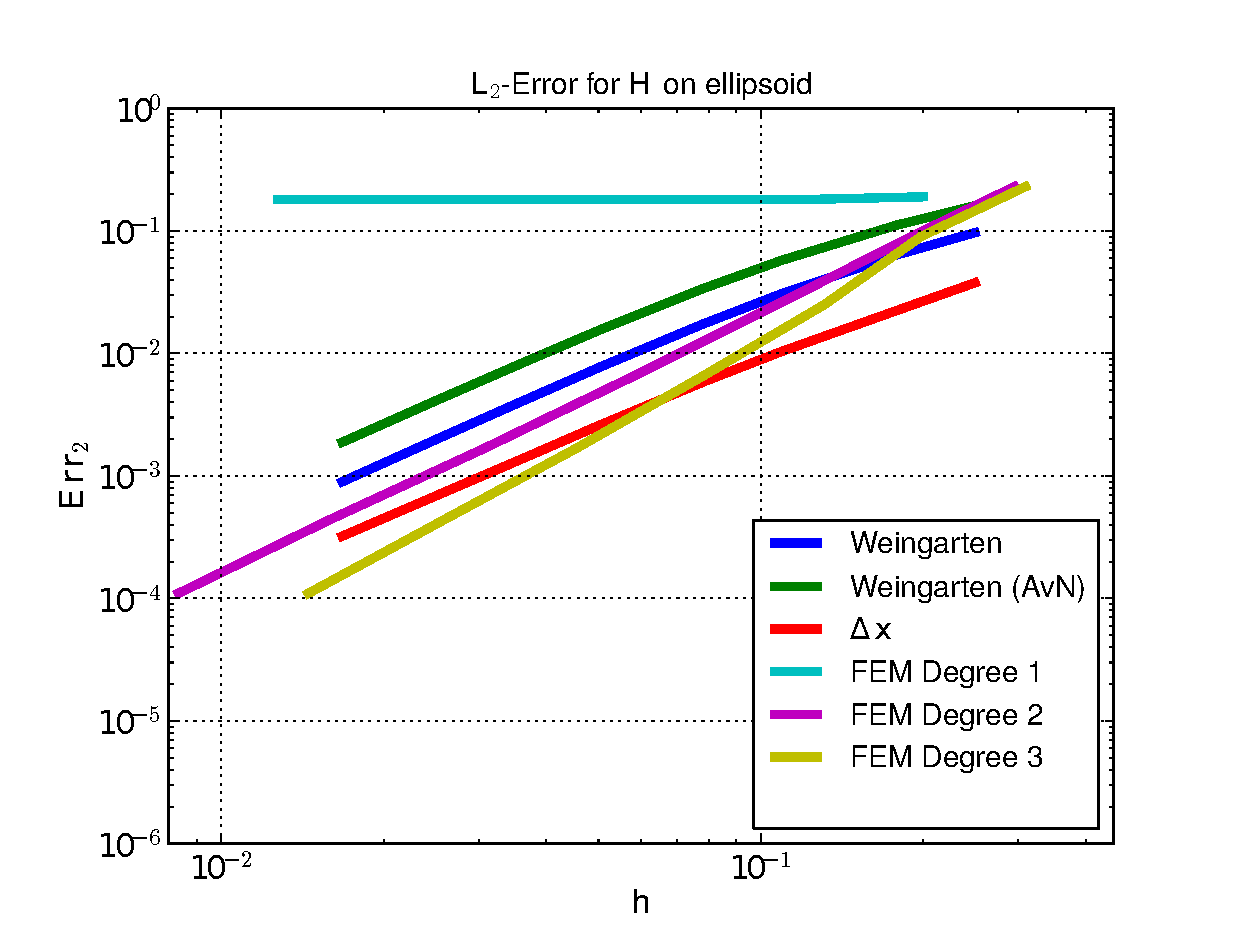
\includegraphics[width=\textwidth]{bilder/Curvature/heineC/ErrHL2_6.eps}
          \end{minipage}
      \onslide<15> 
          \begin{minipage}[t]{0.49\textwidth}
            \centering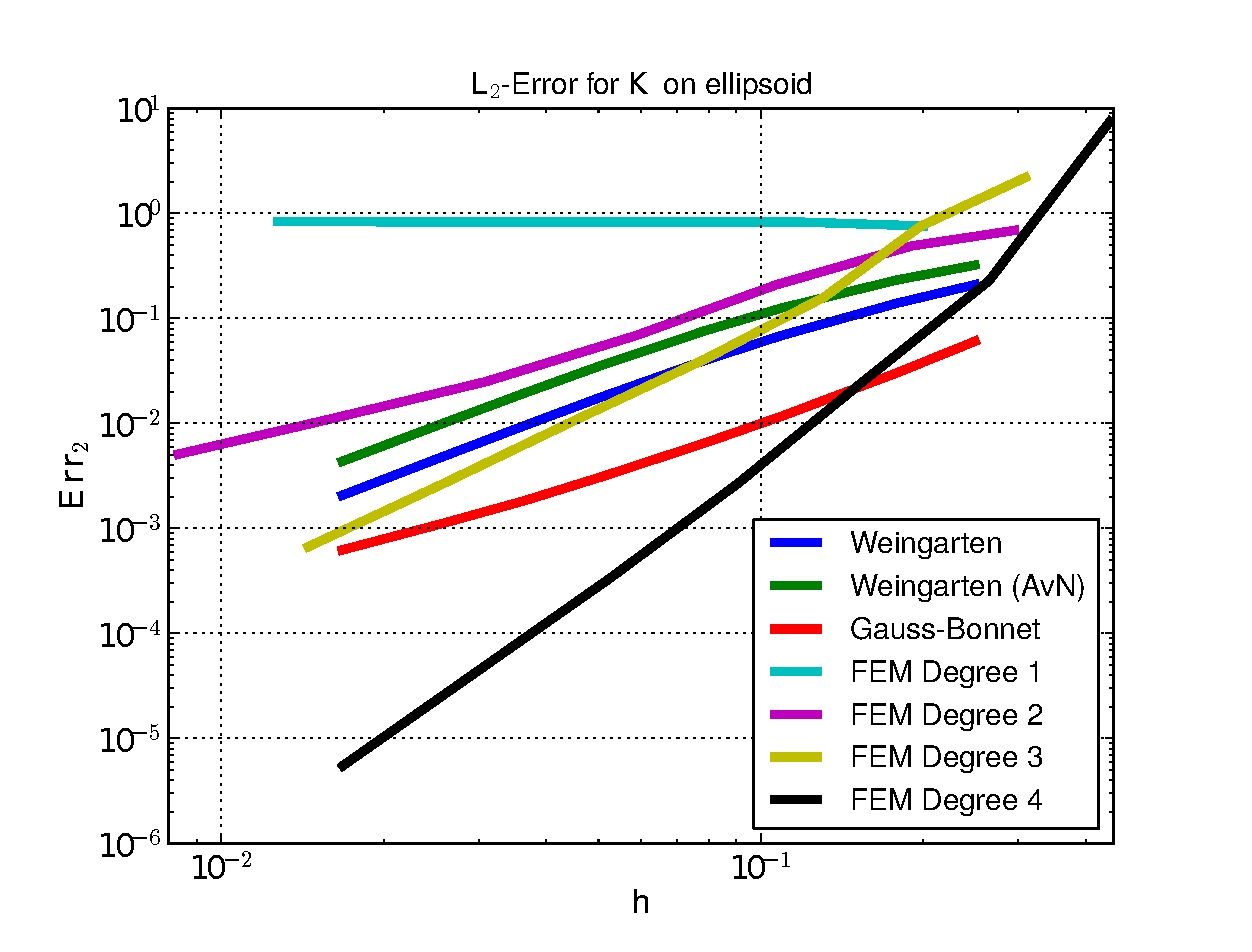
\includegraphics[width=\textwidth]{bilder/Curvature/heineC/ErrKL2_7.eps}
          \end{minipage}\hfill
          \begin{minipage}[t]{0.49\textwidth}
            \centering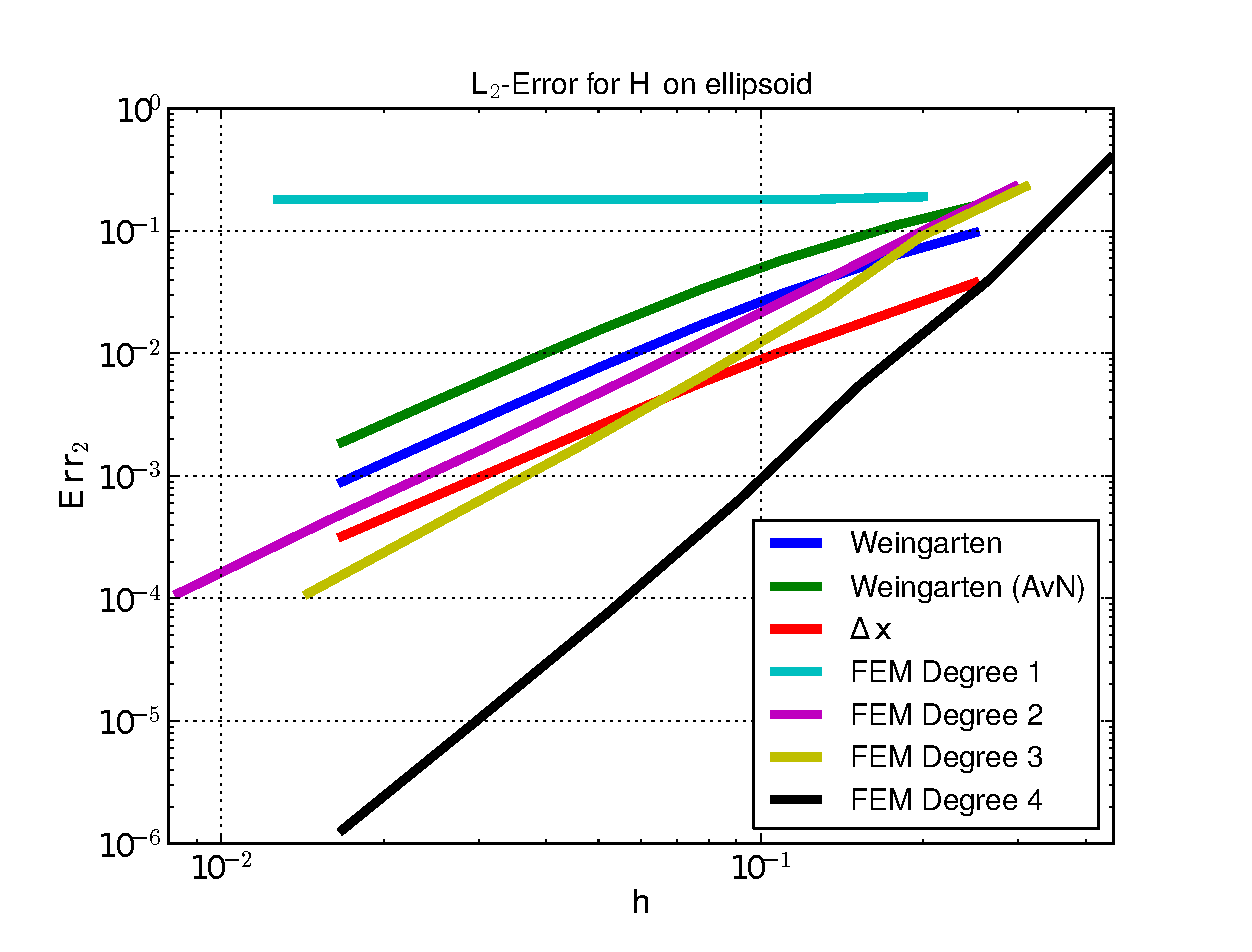
\includegraphics[width=\textwidth]{bilder/Curvature/heineC/ErrHL2_7.eps}
          \end{minipage}
      %quartic S
      \onslide<16> 
          \begin{minipage}[t]{0.49\textwidth}
              \centering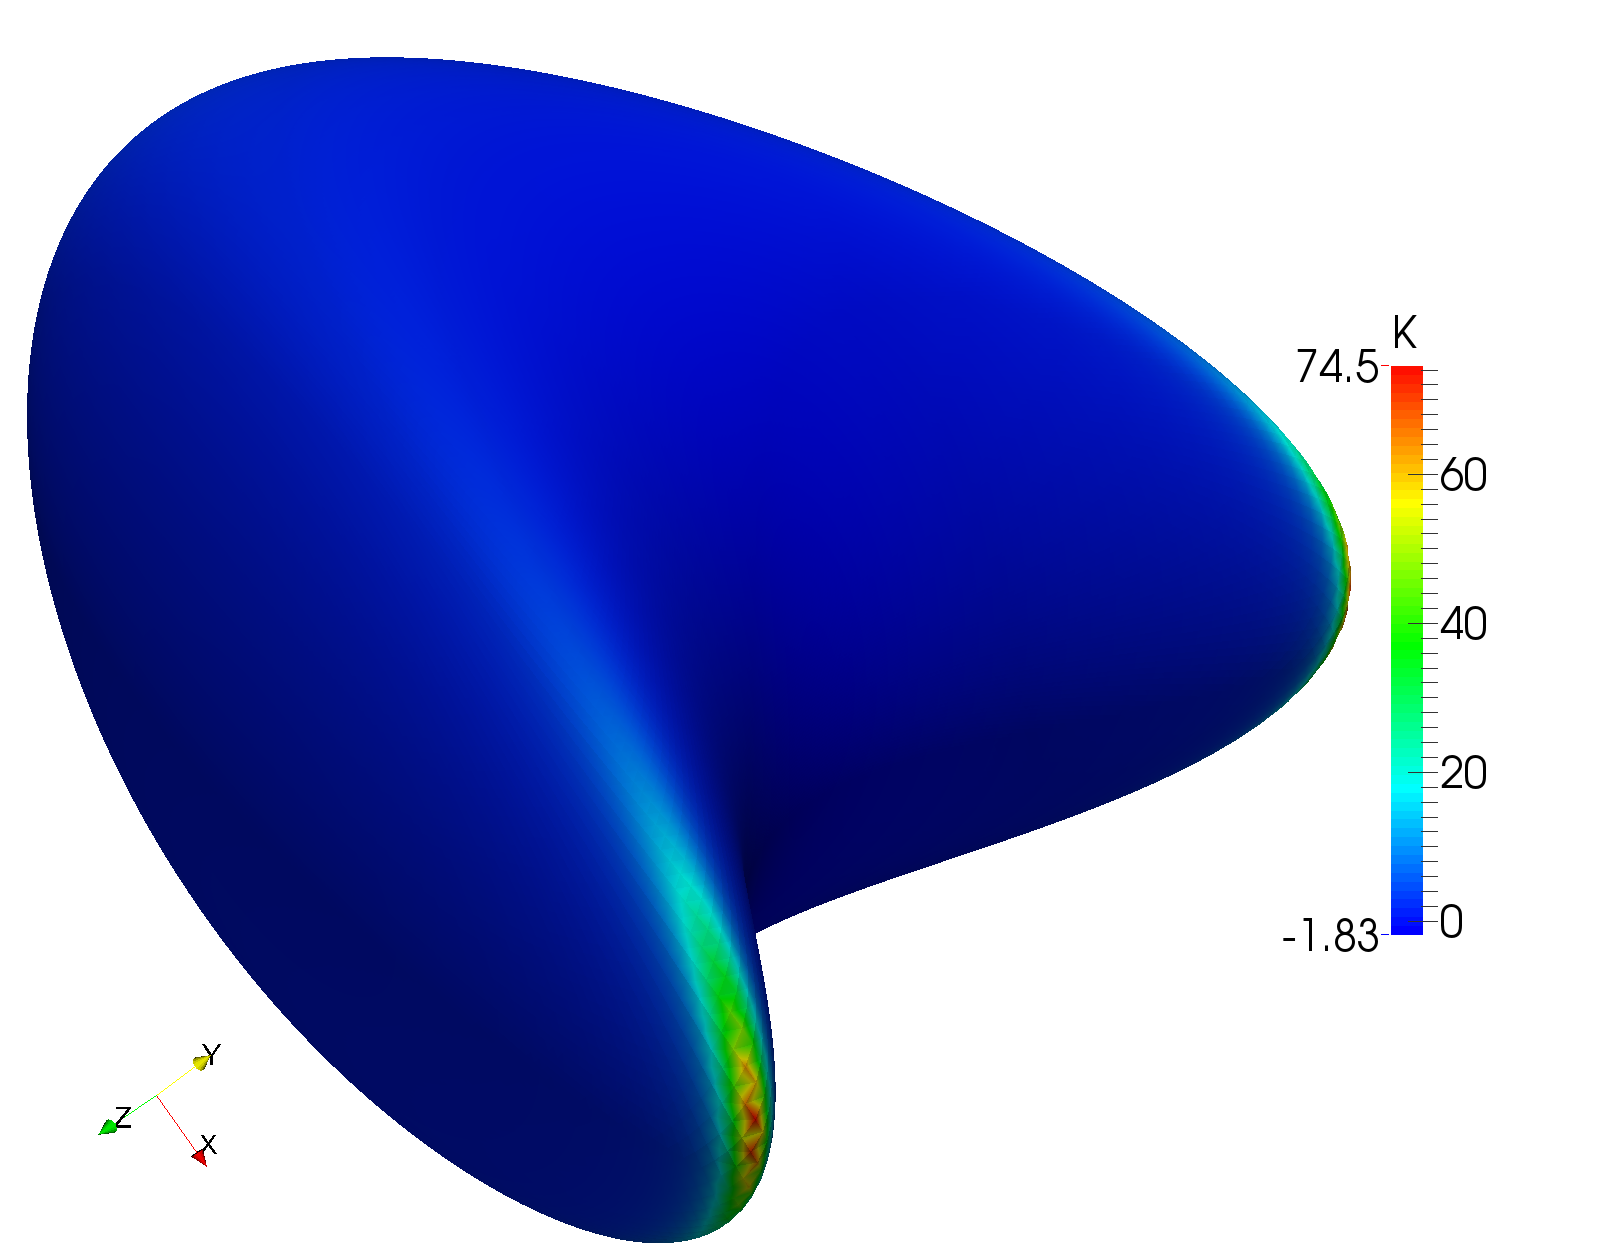
\includegraphics[width=\textwidth]{bilder/Curvature/heineB/K250k.png}
          \end{minipage}\hfill
          \begin{minipage}[t]{0.49\textwidth}
              \centering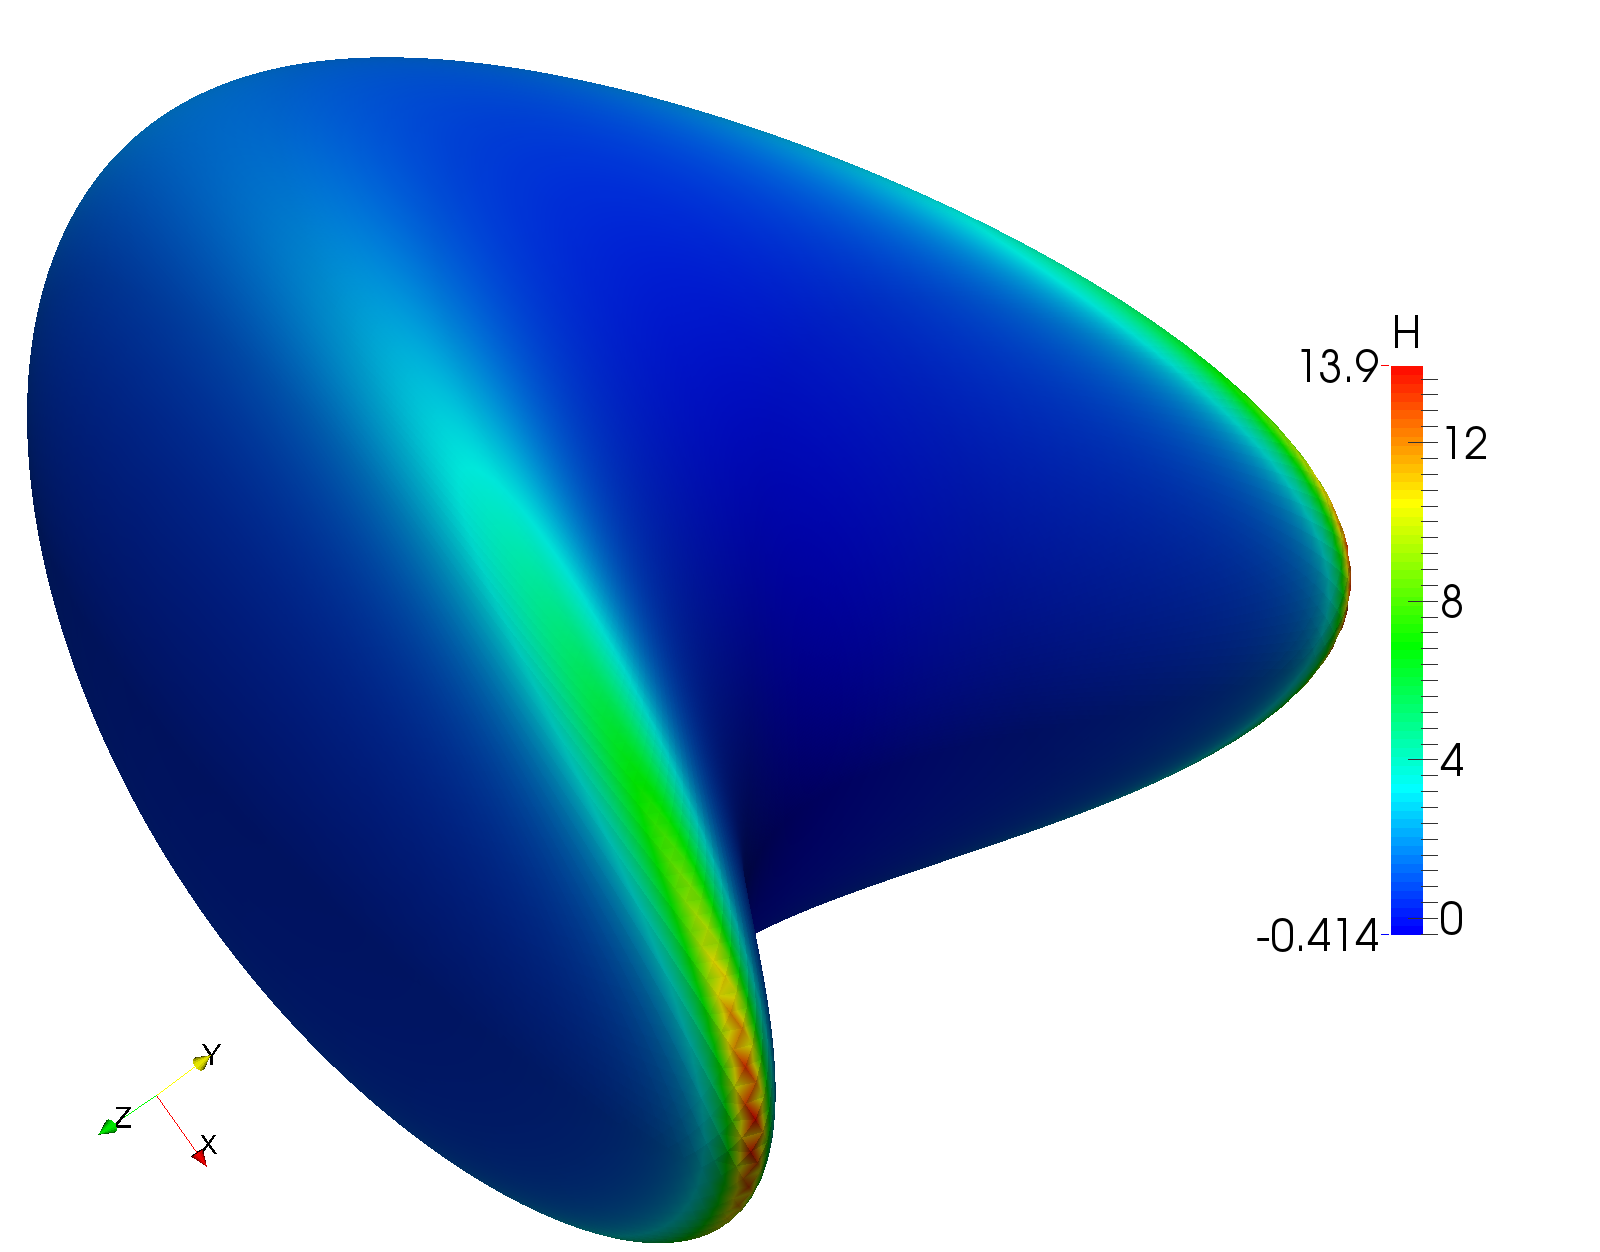
\includegraphics[width=\textwidth]{bilder/Curvature/heineB/H250k.png}
          \end{minipage}
      \onslide<17> 
          \begin{minipage}[t]{0.49\textwidth}
            \centering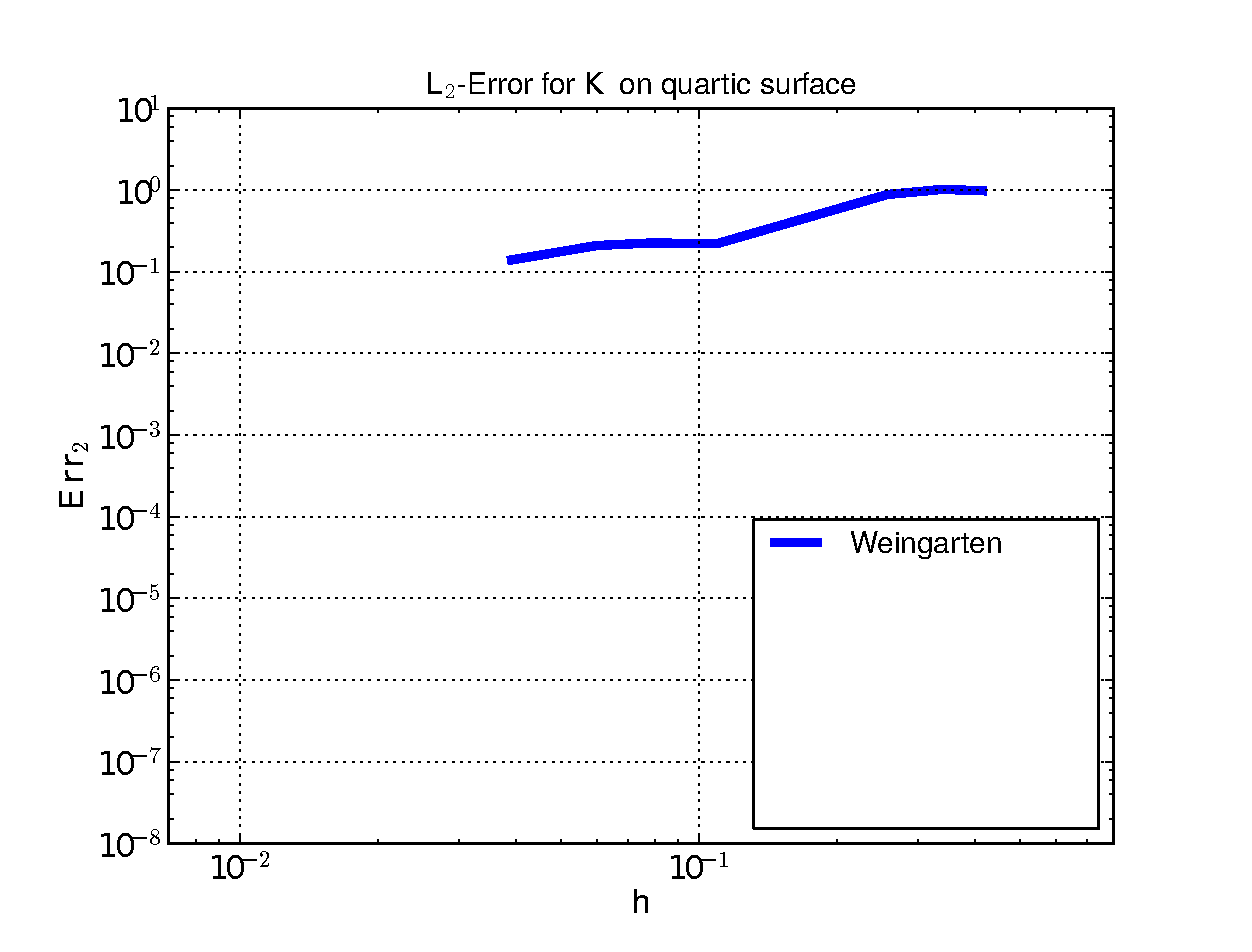
\includegraphics[width=\textwidth]{bilder/Curvature/heineB/ErrKL2_1.eps}
          \end{minipage}\hfill
          \begin{minipage}[t]{0.49\textwidth}
            \centering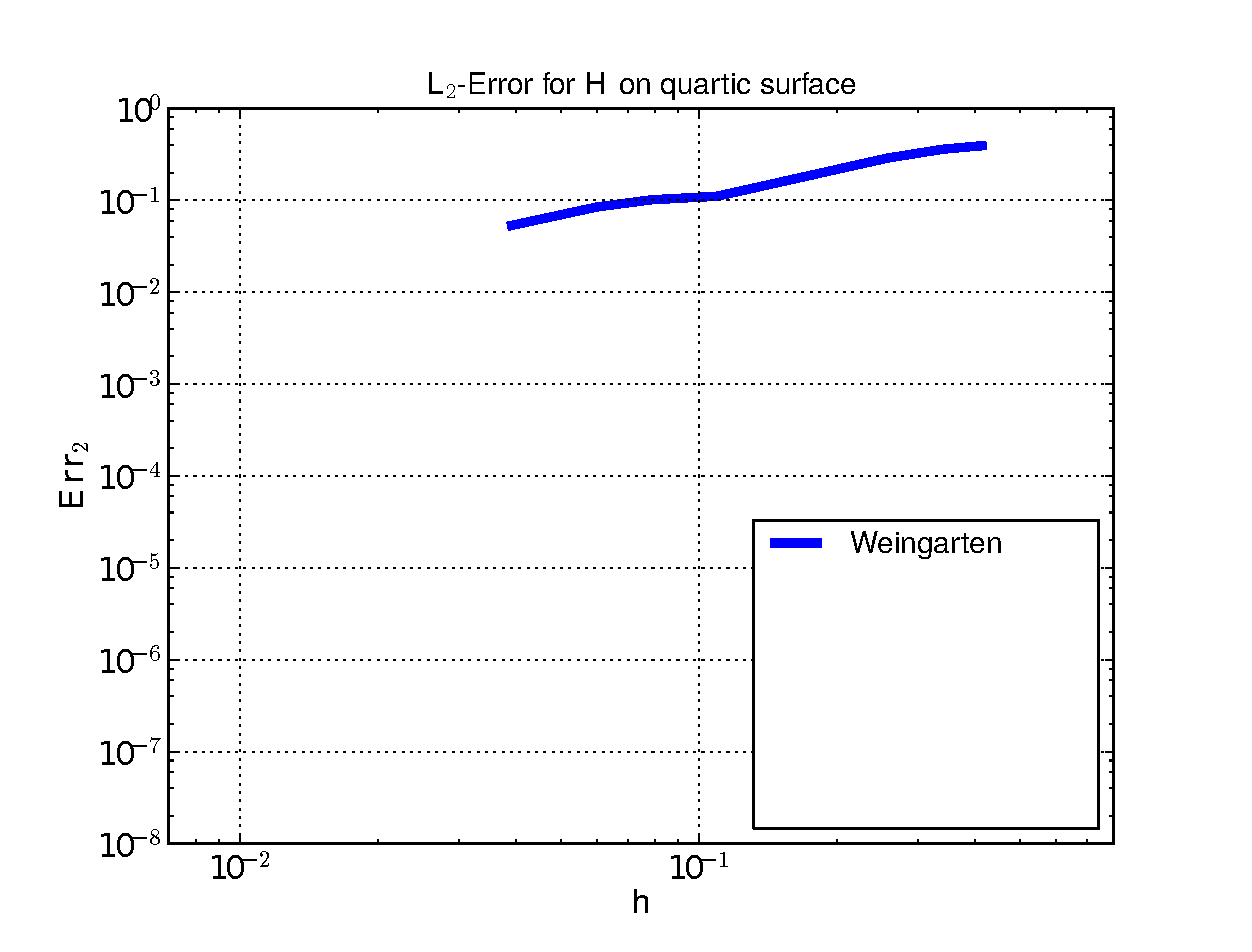
\includegraphics[width=\textwidth]{bilder/Curvature/heineB/ErrHL2_1.eps}
          \end{minipage}
      \onslide<18> 
          \begin{minipage}[t]{0.49\textwidth}
            \centering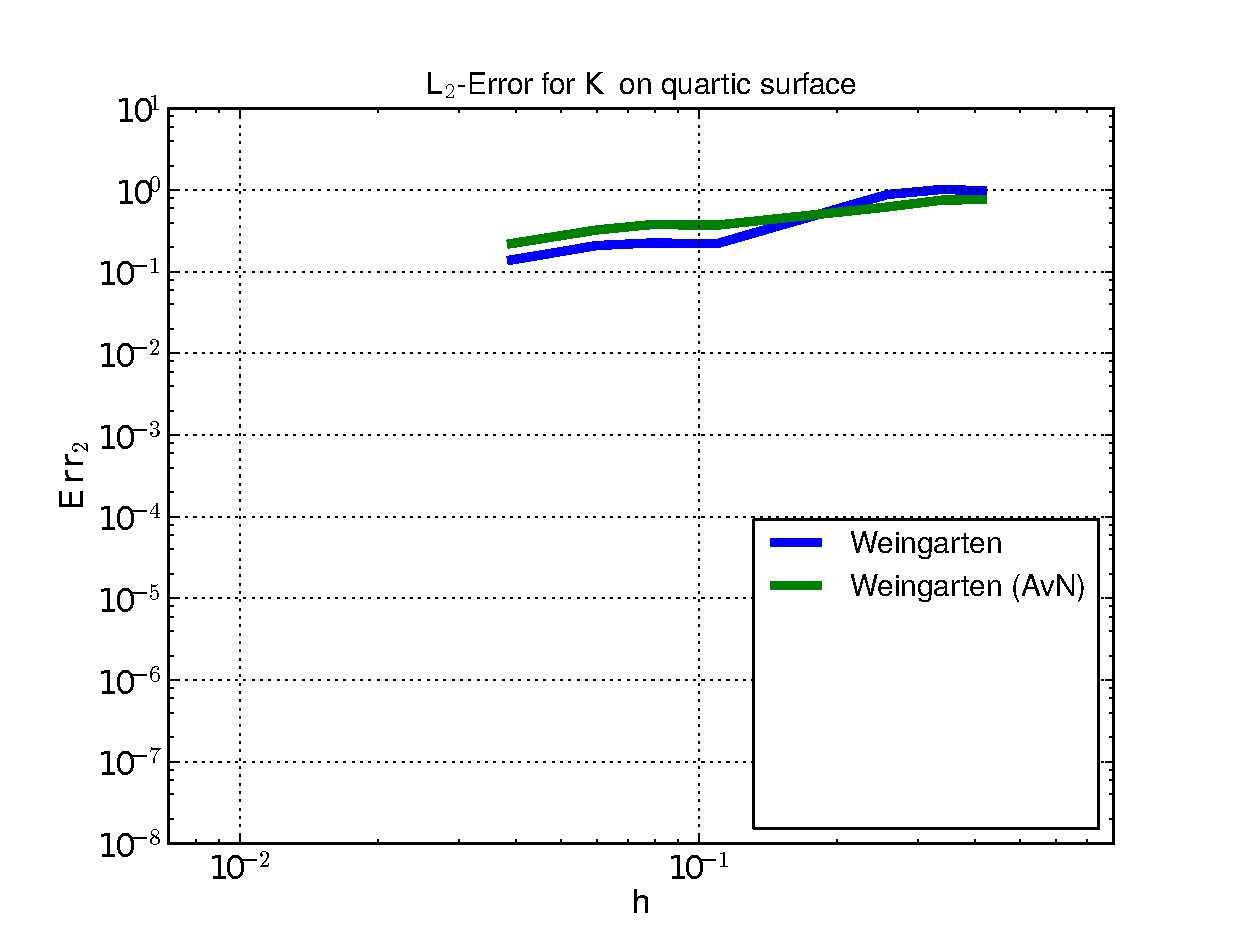
\includegraphics[width=\textwidth]{bilder/Curvature/heineB/ErrKL2_2.eps}
          \end{minipage}\hfill
          \begin{minipage}[t]{0.49\textwidth}
            \centering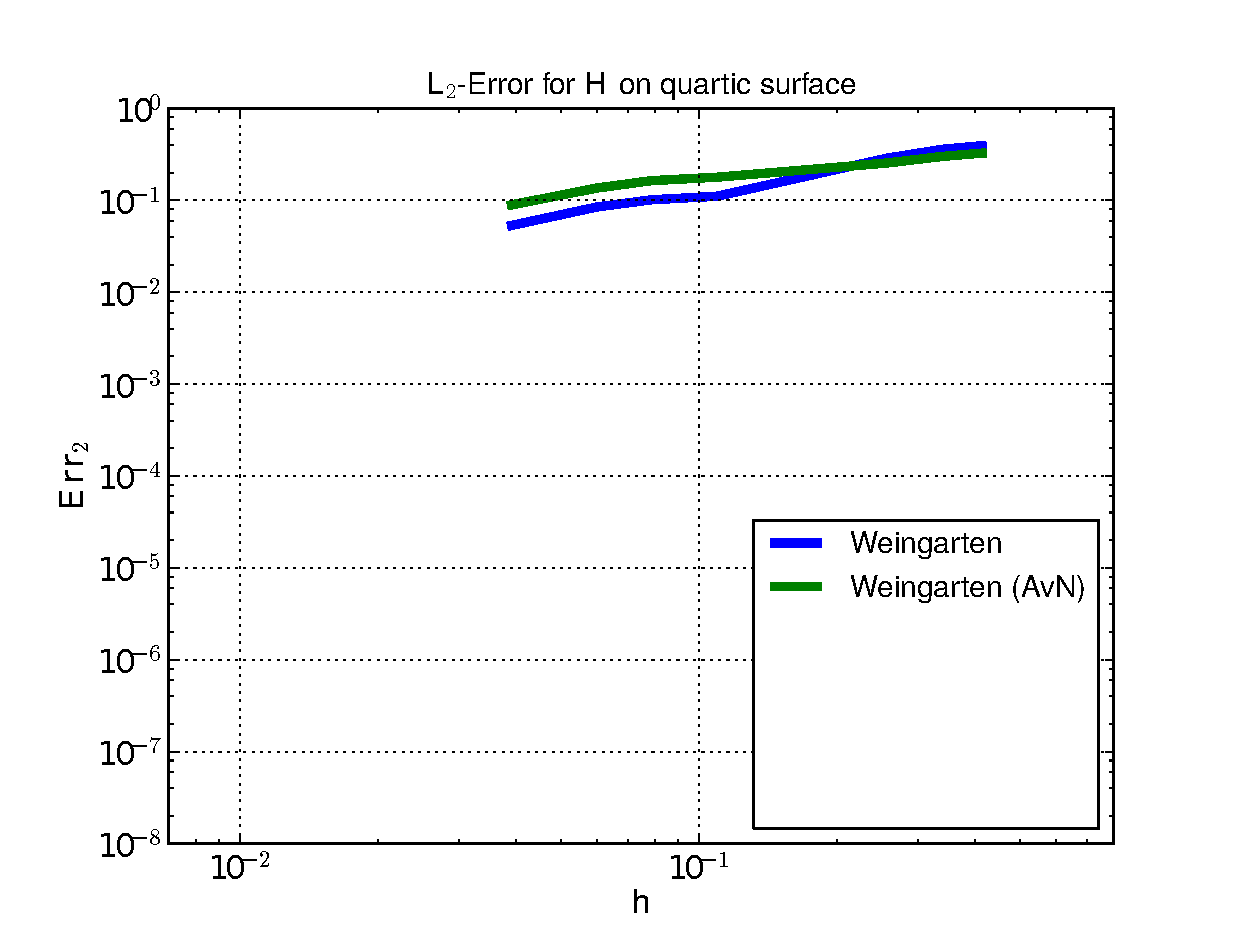
\includegraphics[width=\textwidth]{bilder/Curvature/heineB/ErrHL2_2.eps}
          \end{minipage}
      \onslide<19> 
          \begin{minipage}[t]{0.49\textwidth}
            \centering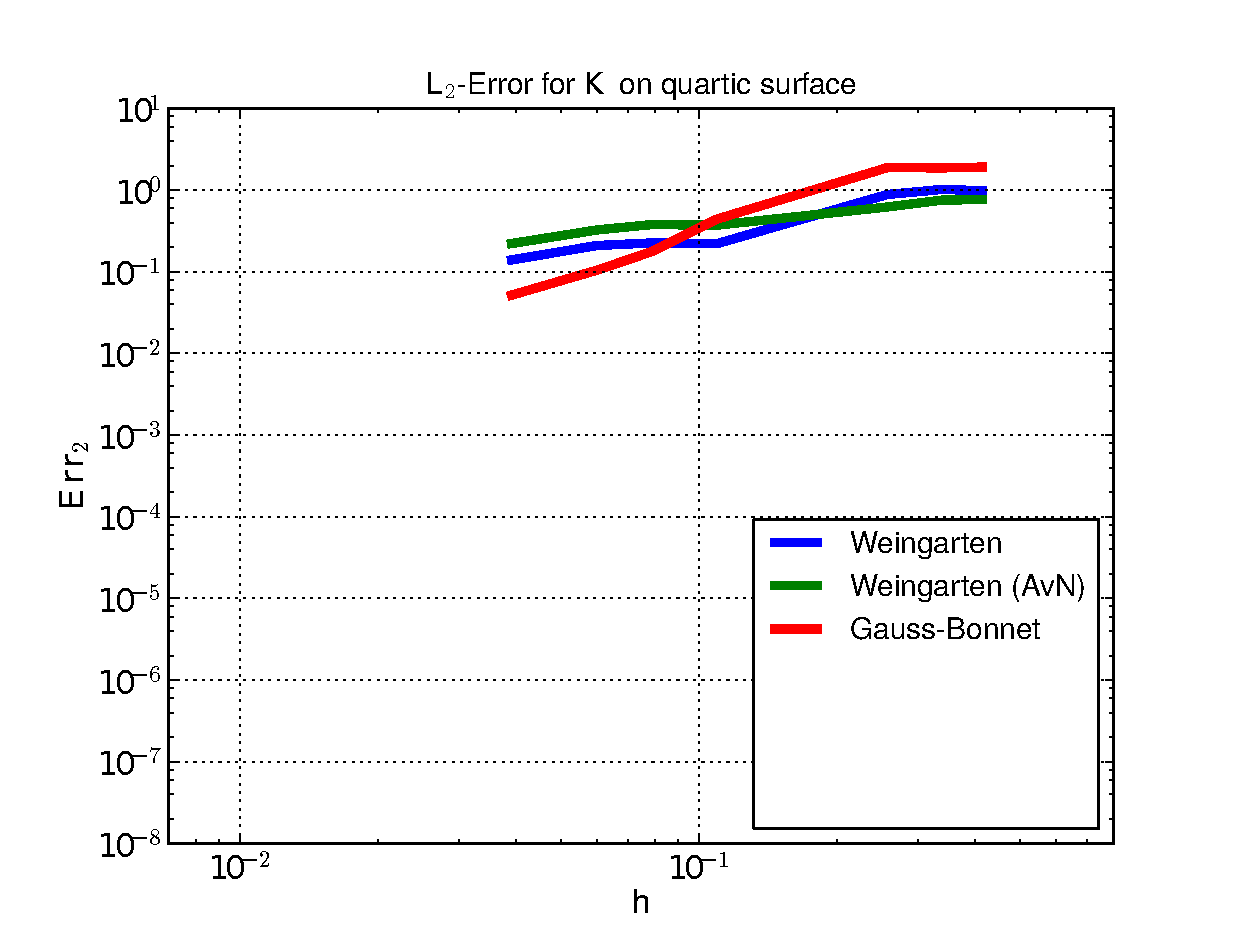
\includegraphics[width=\textwidth]{bilder/Curvature/heineB/ErrKL2_3.eps}
          \end{minipage}\hfill
          \begin{minipage}[t]{0.49\textwidth}
            \centering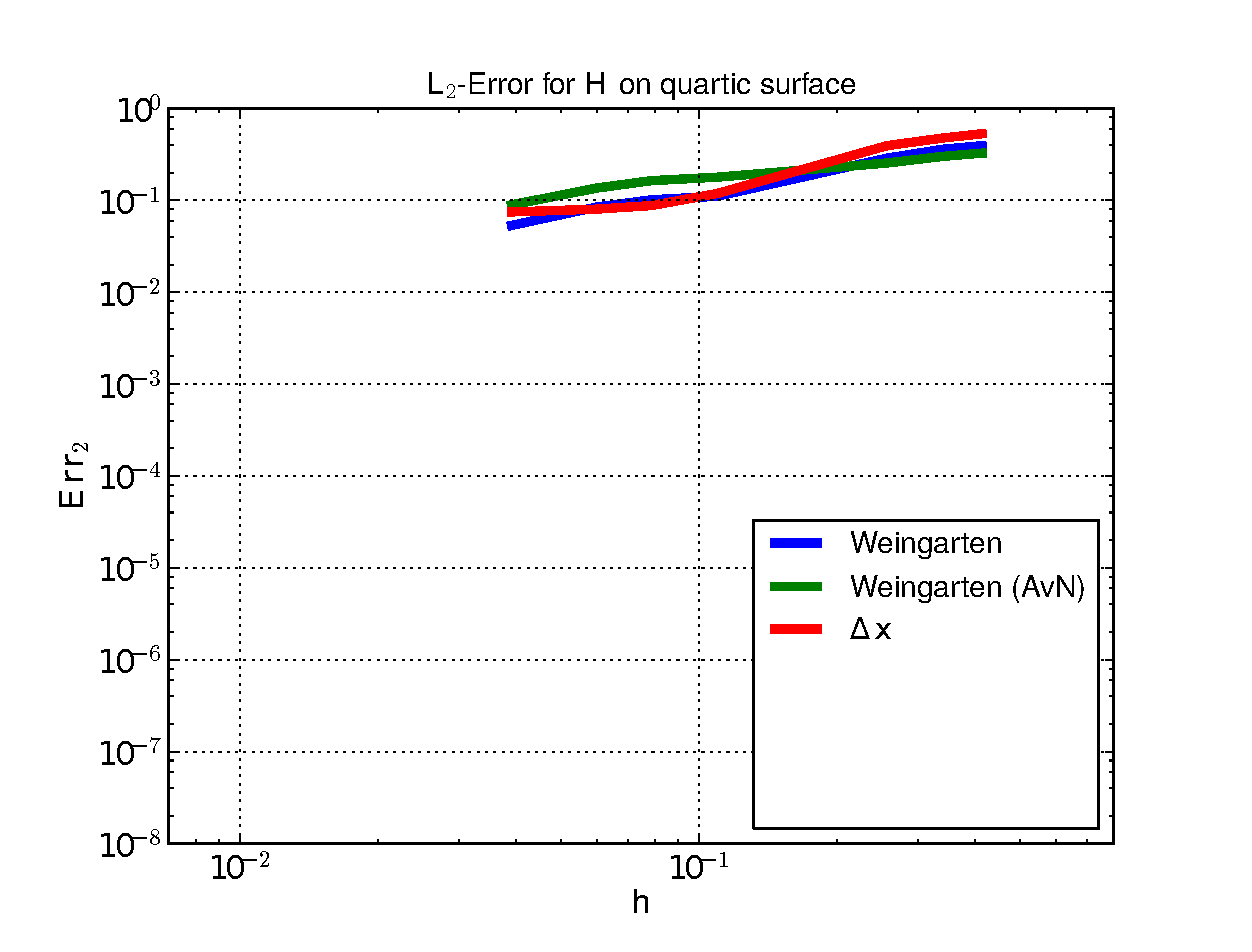
\includegraphics[width=\textwidth]{bilder/Curvature/heineB/ErrHL2_3.eps}
          \end{minipage}
      \onslide<20> 
          \begin{minipage}[t]{0.49\textwidth}
            \centering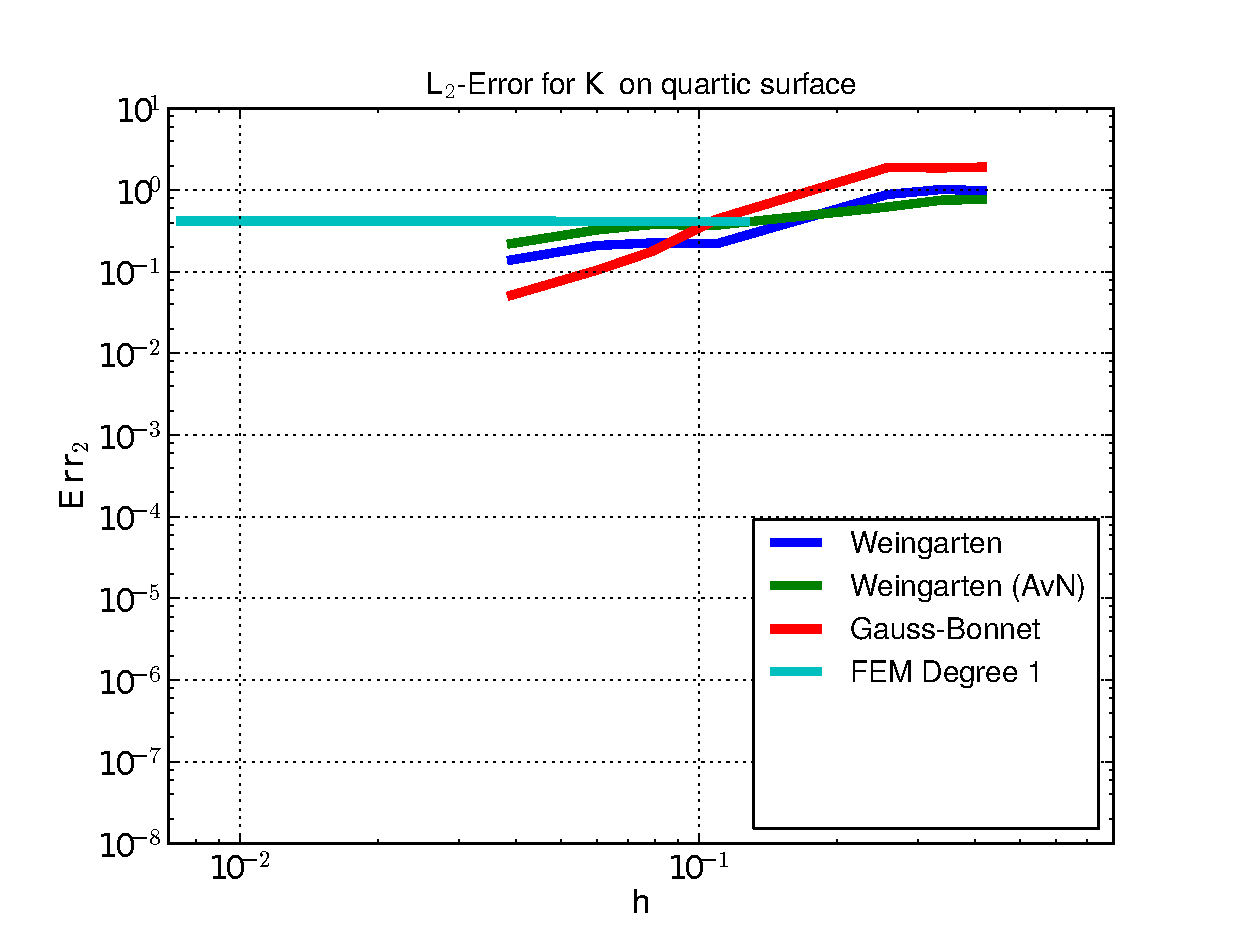
\includegraphics[width=\textwidth]{bilder/Curvature/heineB/ErrKL2_4.eps}
          \end{minipage}\hfill
          \begin{minipage}[t]{0.49\textwidth}
            \centering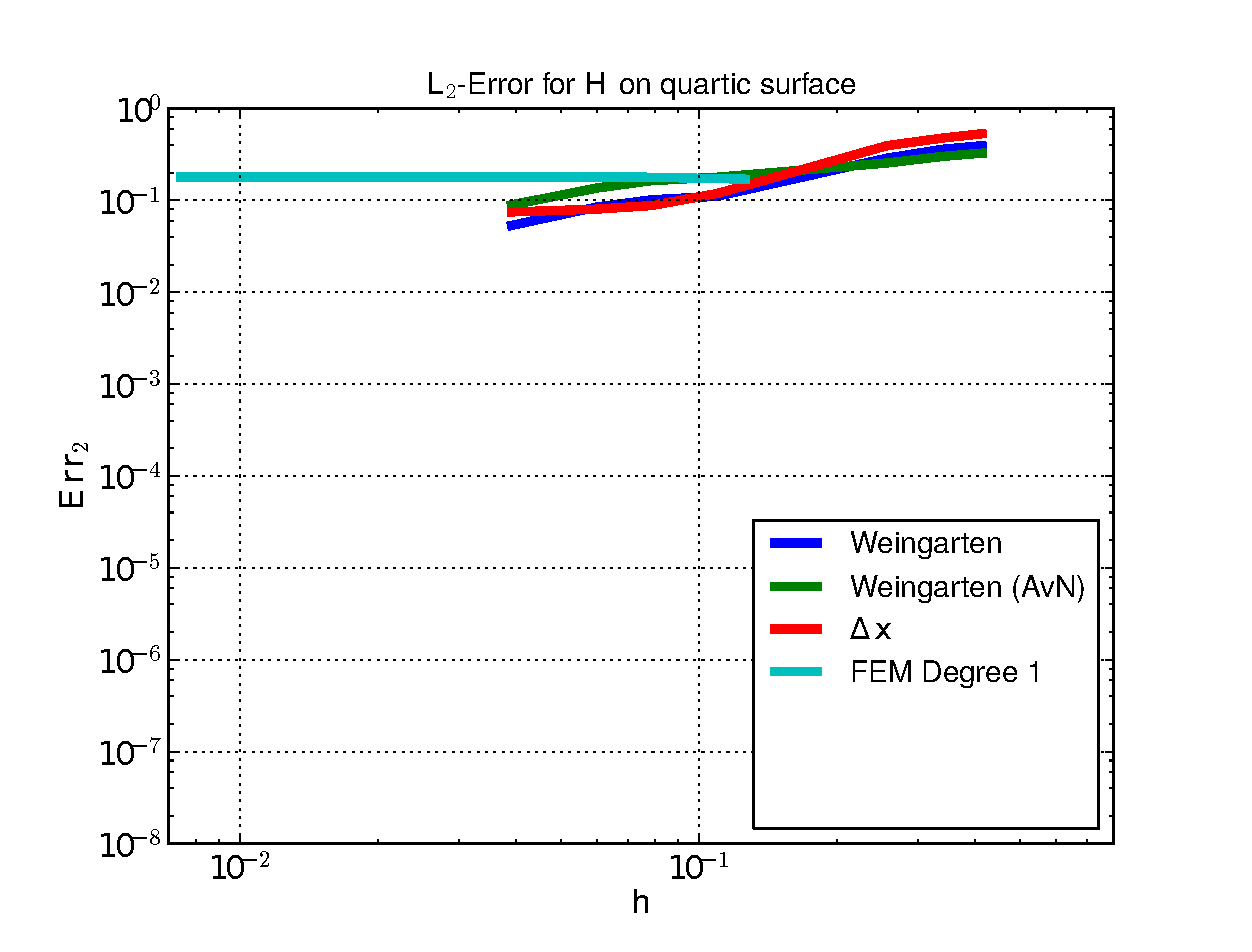
\includegraphics[width=\textwidth]{bilder/Curvature/heineB/ErrHL2_4.eps}
          \end{minipage}
      \onslide<21> 
          \begin{minipage}[t]{0.49\textwidth}
            \centering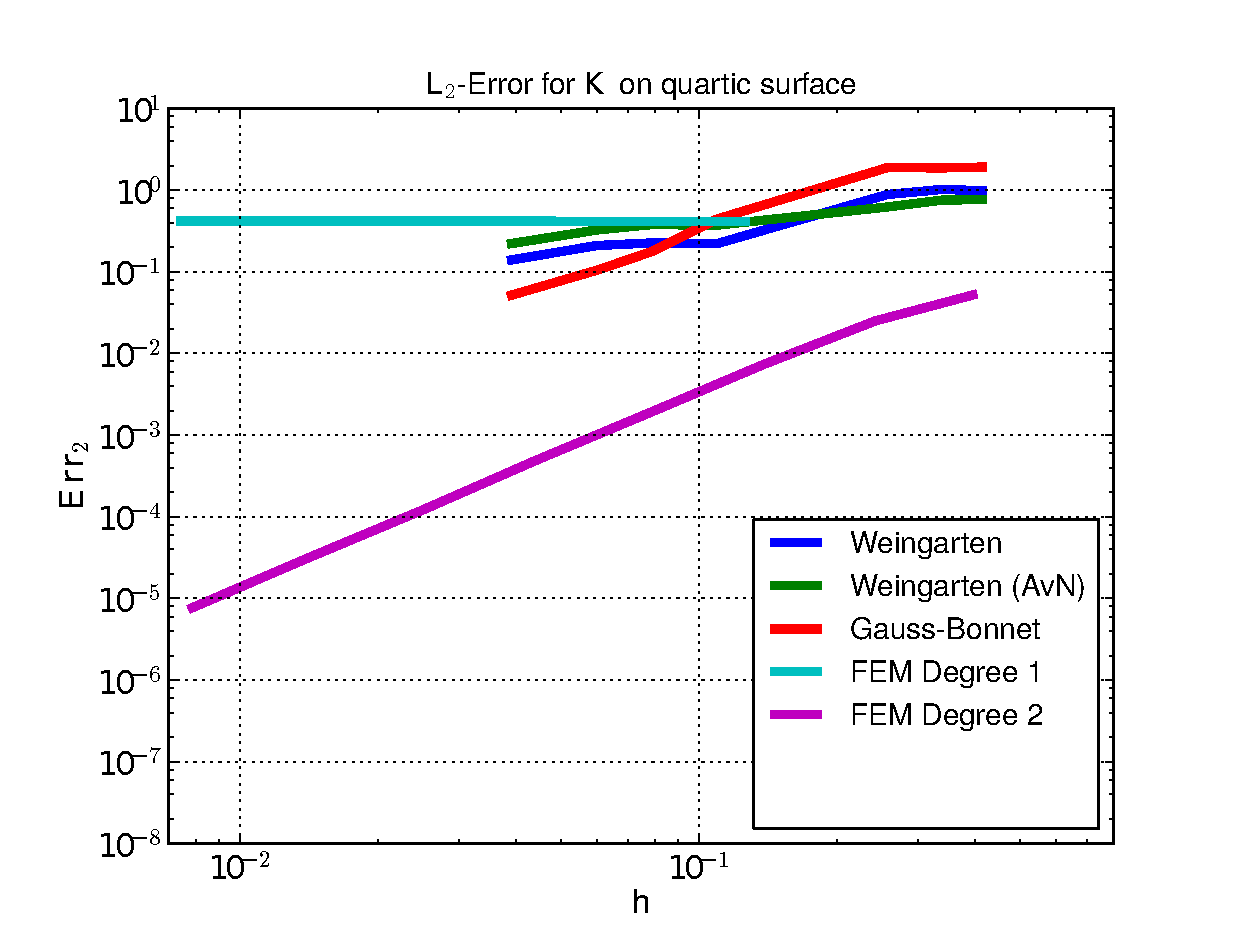
\includegraphics[width=\textwidth]{bilder/Curvature/heineB/ErrKL2_5.eps}
          \end{minipage}\hfill
          \begin{minipage}[t]{0.49\textwidth}
            \centering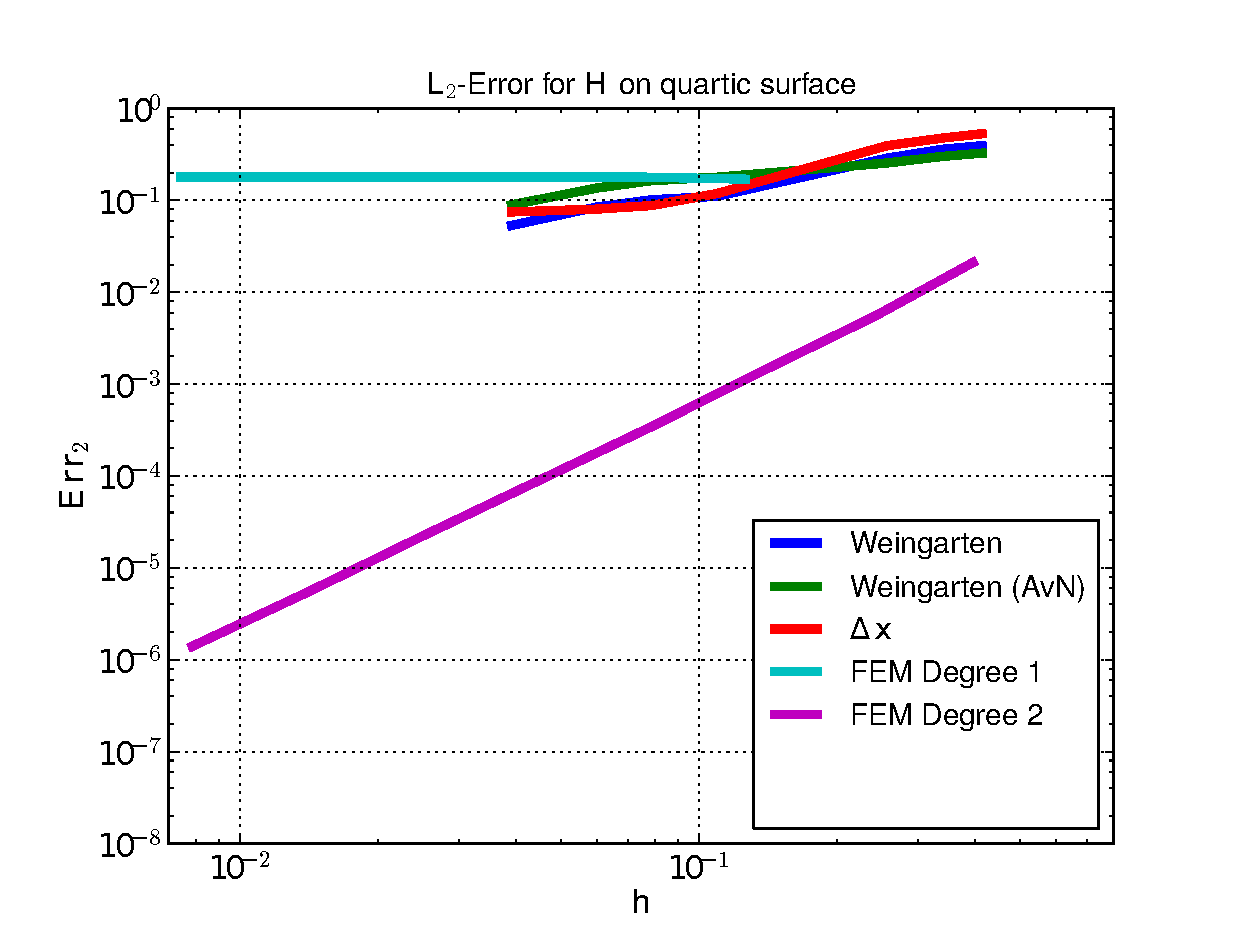
\includegraphics[width=\textwidth]{bilder/Curvature/heineB/ErrHL2_5.eps}
          \end{minipage}
      \onslide<22> 
          \begin{minipage}[t]{0.49\textwidth}
            \centering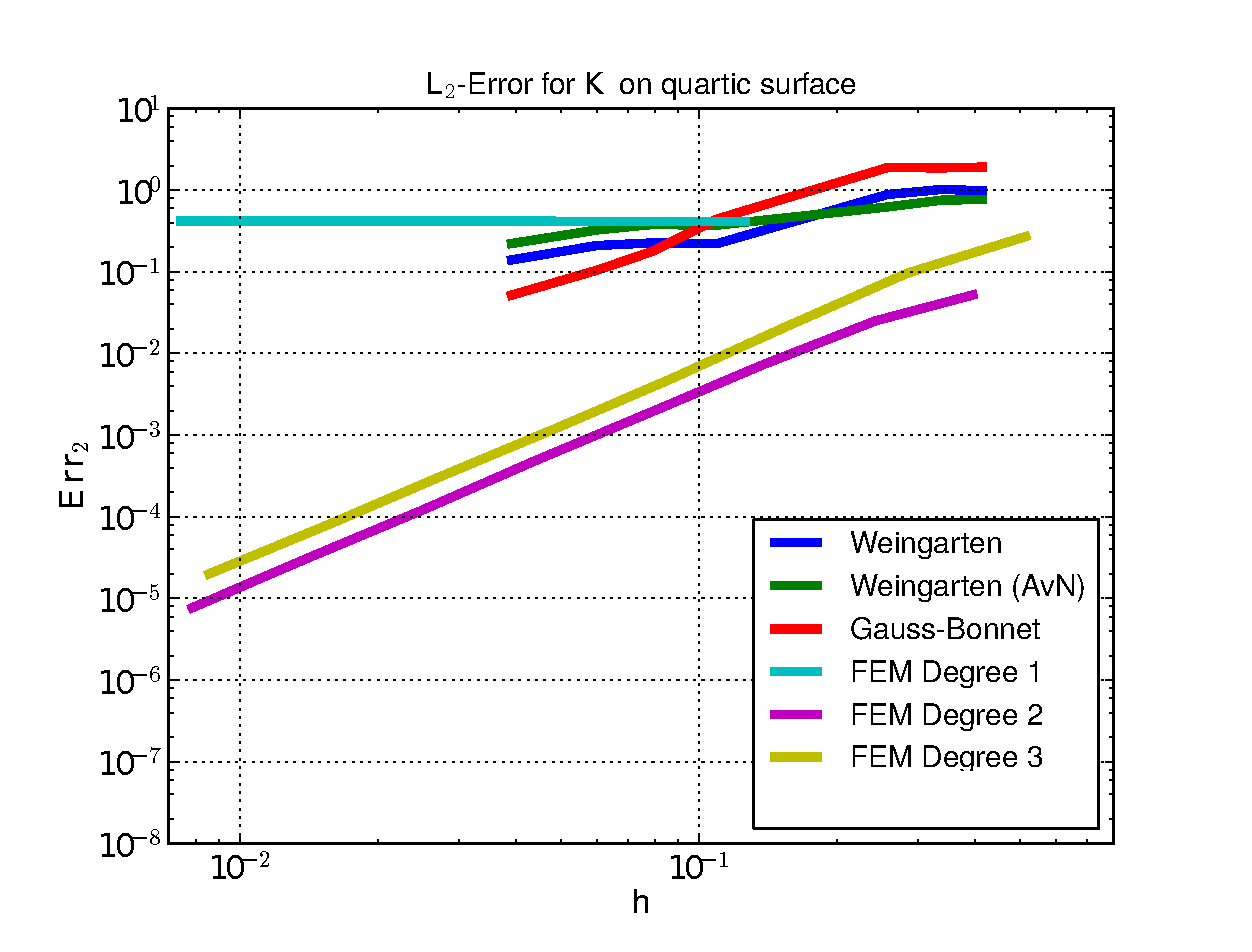
\includegraphics[width=\textwidth]{bilder/Curvature/heineB/ErrKL2_6.eps}
          \end{minipage}\hfill
          \begin{minipage}[t]{0.49\textwidth}
            \centering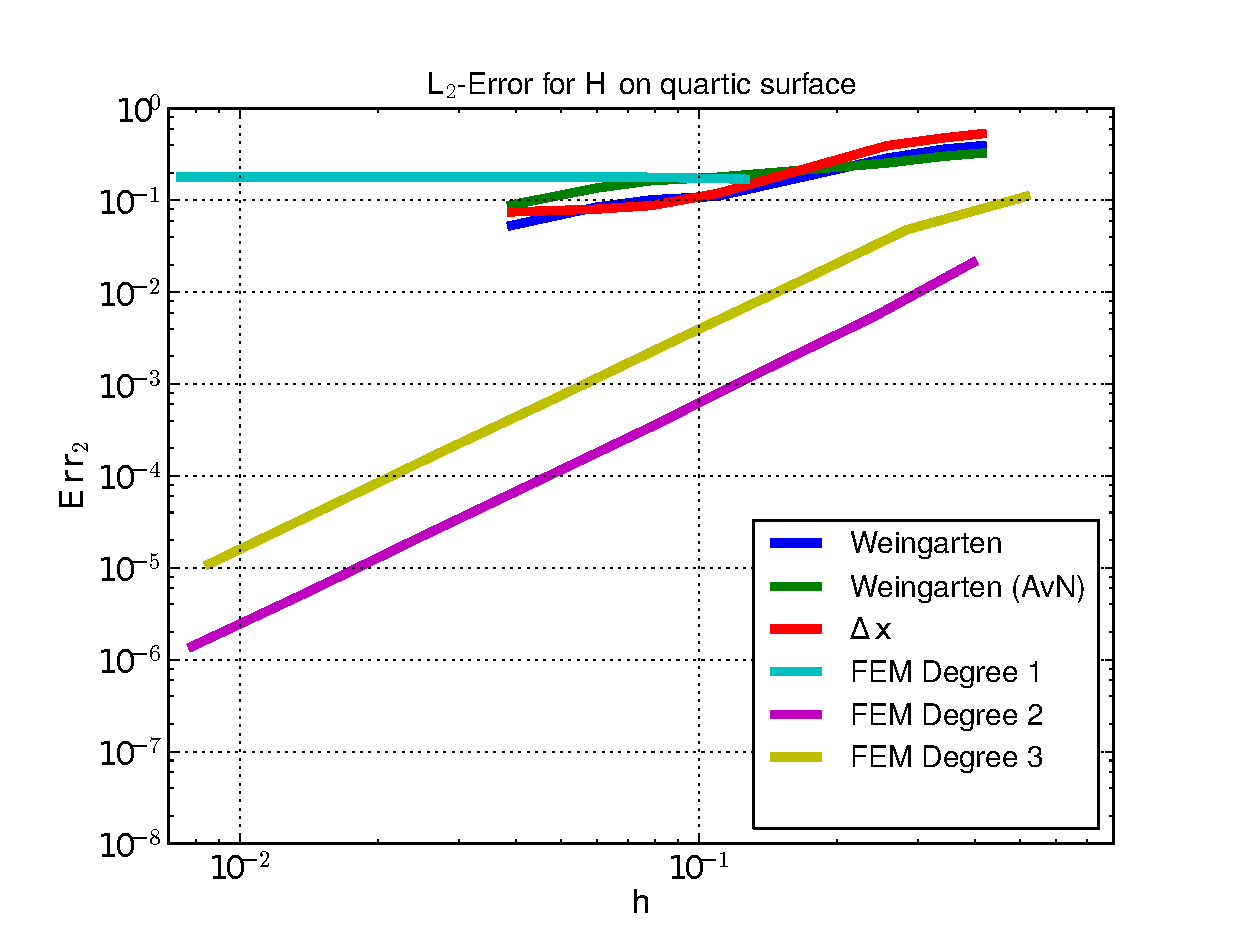
\includegraphics[width=\textwidth]{bilder/Curvature/heineB/ErrHL2_6.eps}
          \end{minipage}
      \onslide<23> 
          \begin{minipage}[t]{0.49\textwidth}
            \centering\includegraphics[width=\textwidth]{bilder/Curvature/heineB/ErrKL2_7.eps}
          \end{minipage}\hfill
          \begin{minipage}[t]{0.49\textwidth}
            \centering\includegraphics[width=\textwidth]{bilder/Curvature/heineB/ErrHL2_7.eps}
          \end{minipage}
    \end{overprint}
  \end{frame}

\section{Fazit und Ausblicke}

  \begin{frame}
    \begin{block}{Pros}
      \begin{itemize}
        \item Äußeres Kalkül (Problemformulierung)
        %\item Unabhängigkeit der Ambientedimension
        \item Geringer Aufwand im Vergleich zu Diffuse Domain Ansätzen 
        \item Geringer Aufwand der Krümmungsberechnung im Vergleich zur isoparametrischen FEM
        \item Gute Integration in AMDiS
      \end{itemize}
    \end{block}
    \pause
    \begin{block}{Kontras}
      \begin{itemize}
        \item Äußeres Kalkül (Flat, Sharp)
        \item Wohlzentriertheit
        \item Lineare Approximation der Mannigfaltigkeit
        %lineare oberflächenapprox--- keine tangentialräume
      \end{itemize}
    \end{block}
  \end{frame}

  \begin{frame}
    \begin{block}{\huge Vielen Dank für Ihre Aufmerksamkeit! }
      \centering\href{run:videos/defSphere/runVideo.sh}{\includegraphics[width=0.8\textwidth]{videos/defSphere/defSphere.png}}
    \end{block}
  \end{frame}

  \begin{frame}
    \begin{block}{Ausgewählte Literatur}
      \footnotesize
      \nocite{hirani}\nocite{marsden}\nocite{jaenich}\nocite{meshCooper}
      \bibliographystyle{alpha}
      \bibliography{bibl.bib}{}
    \end{block}
  \end{frame}

\end{document}
